\documentclass[a4paper,12pt]{report}

% ╔═════════════════════════════════════════════════════════════════════
%                         ISTRUZIONI PER LA COMPILAZIONE     
%                       
%                      usare \showimagestrue - \showimagestrue
% ╚═════════════════════════════════════════════════════════════════════

\newif\ifshowimages
\showimagestrue% ← CAMBIA QUI: \showimagesfalse (veloce) | \showimagestrue (completo)

% ─────────────────────────────────────────────────────────────────────────────

% 1. Encoding and Language (Babel first)
\usepackage[utf8]{inputenc}
\usepackage[T1]{fontenc} 
\usepackage[english,italian]{babel}
\usepackage{lmodern} 

% 2. Math and Graphics
\usepackage{amsmath, amssymb, amsfonts}
\ifshowimages
  \usepackage{graphicx}
\else
  \usepackage[draft]{graphicx}
\fi
\usepackage{svg}
\usepackage{float}
\usepackage{tikz}
\usetikzlibrary{shapes.geometric}
\usepackage{pgfplots}
\pgfplotsset{compat=1.18}
\usepackage{pgf-pie}

% 3. Layout and Utilities
\usepackage[left=2.5cm, right=2cm, top=2cm, bottom=2cm]{geometry}
\usepackage{setspace}
\usepackage{enumitem}
\usepackage{array}
\usepackage{tabularx}
\usepackage{subcaption}
\usepackage{xcolor}
\usepackage{titlesec}

% 4. Footnotes and Typography (Footmisc BEFORE Microtype)
\usepackage{footmisc}
\usepackage{microtype}

% 5. Code Listings
\usepackage{listings}
\definecolor{backcolour}{rgb}{0.95,0.95,0.92}
\lstset{
    backgroundcolor=\color{backcolour},
    basicstyle=\ttfamily\footnotesize,
    breaklines=true,
    frame=single,
    columns=flexible
}

% 6. Links and URLs (Hyperref and Xurl ALWAYS last)
\usepackage{xurl}
\usepackage[hidelinks]{hyperref}

% --- Custom Formatting ---

% Formattazione Titoli
\titleformat{\chapter}[hang]
  {\normalfont\huge\bfseries}
  {\thechapter.}{1em}{}

% Impostazioni paragrafo
\setlength{\parindent}{0pt} 
\setstretch{1.2}
\setlength{\parskip}{8pt}

% --- Document Data ---

\title{Progetto di Interazione Uomo-Macchina\\ \large Analisi dell'Usabilità e Riprogettazione del sito "Guided Tours"}
\author{Daniel Barbetti\\Marco Cesari\\Felappi Giorgio}
\date{\today}

% --- Main Content ---

\begin{document}

\maketitle
\thispagestyle{empty}

\renewcommand{\contentsname}{Indice}
\tableofcontents

% Inclusione dei capitoli
\chapter{Introduzione e Descrizione del Sistema}
\label{cap:intro}

\section{Panoramica dell'Applicazione}
Il progetto oggetto di questa relazione, denominato \textbf{Guided Tours}, consiste nella progettazione e nello sviluppo di un'applicazione web orientata alla gestione di visite guidate. Il sistema è stato concepito per rispondere alle esigenze di organizzazioni locali senza scopo di lucro che si occupano della valorizzazione del patrimonio territoriale, sia esso di natura storico-artistica che paesaggistica.

L'obiettivo primario della piattaforma è la digitalizzazione del flusso organizzativo che intercorre tra la domanda, rappresentata da visitatori singoli o gruppi (scuole, turisti), e l'offerta, costituita da una rete di guide volontarie. Attualmente, tali processi sono spesso gestiti in modo frammentato e manuale; il sistema proposto mira a centralizzare le informazioni, ottimizzare l'assegnazione delle risorse umane e garantire un canale di comunicazione strutturato.

L'architettura logica dell'applicazione prevede tre attori principali, ciascuno caratterizzato da specifici privilegi e interfacce dedicate:
\begin{itemize}
    \item \textbf{Fruitore:} L'utente esterno che naviga il catalogo delle offerte culturali e inoltra richieste di prenotazione. Può agire come singolo o come capogruppo.
    \item \textbf{Volontario:} La risorsa operativa dell'organizzazione. Accede al sistema per comunicare le proprie disponibilità temporali e le proprie competenze (es. lingue parlate, abilitazioni per specifici luoghi).
    \item \textbf{Configuratore:} Il ruolo amministrativo che detiene il controllo completo del sistema. Si occupa del popolamento delle anagrafiche (Luoghi, Tipologie di Visita) e della gestione operativa delle richieste, incrociando le esigenze dei fruitori con le disponibilità dei volontari.
\end{itemize}

\section{Analisi dell'Interfaccia e Funzionalità}
L'interfaccia utente è stata progettata seguendo i principi di usabilità e chiarezza informativa, differenziando nettamente le aree pubbliche da quelle riservate. Di seguito viene fornita un'analisi dettagliata delle sezioni costitutive del sistema.

\subsection{Landing Page e Navigazione Pubblica}
La Home Page funge da ambiente di accoglienza e snodo direzionale primario per le diverse tipologie di utenza.
Graficamente, il layout è dominato da una sezione introduttiva (\textit{Hero Section}) concepita per comunicare immediatamente la missione dell'organizzazione e instaurare un rapporto di fiducia.
La barra di navigazione superiore è un elemento persistente e offre un \textit{affordance} chiara per l'accesso rapido alle funzioni di autenticazione.

Dal punto di vista dell'analisi dei task, questa vista deve assolvere simultaneamente a due obiettivi:
\begin{enumerate}
    \item \textbf{Informativo (Discovery):} Presentare la proposta di valore ai visitatori anonimi, invitandoli alla conversione (es. registrazione) al fine di prenotare una visita.
    \item \textbf{Direzionale (Routing):} Fornire un accesso immediato e privo di frizioni all'area riservata per lo staff e i volontari già registrati, agendo da \textit{gateway}.
\end{enumerate}

\begin{figure}[H]
    \centering
    % \includegraphics[width=1.0\textwidth]{screenshot_home.png}
    \caption{Landing Page: visualizzazione pubblica con call-to-action per la registrazione.}
    \label{fig:home}
\end{figure}

\subsection{Sistema di Autenticazione e Registrazione}
La gestione degli accessi rappresenta uno snodo critico nel percorso utente. Il modulo di registrazione introduce una scelta logica dirimente sin dal primo contatto: la selezione del ruolo operativo.
In contrasto con i pattern di registrazione generici, l'utente è chiamato a dichiarare esplicitamente se intende fruire del servizio (\textit{Fruitore}) o far parte del network organizzativo (\textit{Volontario}). Questa profilazione precoce determina in modo permanente l'architettura dell'informazione e il layout successivo, personalizzando l'esperienza utente.

Il modulo richiede l'inserimento di dati obbligatori quali:
\begin{itemize}
    \item Nome e Cognome (per l'identificazione nelle liste presenze).
    \item Indirizzo Email (univoco, utilizzato come username).
    \item Password (con criteri minimi di sicurezza).
\end{itemize}

\begin{figure}[H]
    \centering
    % \includegraphics[width=0.7\textwidth]{screenshot_register.png}
    \caption{Modulo di registrazione con selettore per la tipologia di utenza (Fruitore/Volontario).}
    \label{fig:login_register}
\end{figure}

\subsection{Modulo di Richiesta Visita (Area Fruitore)}
A seguito dell'autenticazione, il \textit{Fruitore} interagisce con un'esplicita Call-to-Action che sblocca l'accesso all'ambiente dedicato alla schedulazione delle visite. Da un punto di vista dell'interazione, tale vista si discosta dal classico paradigma del carrello e-commerce in favore di un modulo guidato procedurale per l'inoltro di una "richiesta di servizio". 
Tale approccio minimizza il carico cognitivo dell'operatore, vincolando l'attenzione su input sequenziali mirati e semanticamente raggruppati.

I campi principali, validati per prevenire errori accidentali di sottomissione, richiedono:
\begin{itemize}
    \item \textbf{Dettagli Logistici:} Data preferita per la visita e numero di partecipanti (informazione cruciale per valutare la sostenibilità e il rapporto guida/visitatori).
    \item \textbf{Preferenze Context-Aware:} Selezione della lingua e campo testuale libero per documentare bisogni specifici del gruppo (es. accessibilità per disabilità motorie), promuovendo un design inclusivo.
\end{itemize}
Al completamento del flusso, il sistema fornisce un feedback contestuale di presa in carico, ponendo la pratica nello stato di sospeso in attesa di validazione asincrona da parte dell'amministrazione.

\begin{figure}[H]
    \centering
    % \includegraphics[width=0.8\textwidth]{screenshot_booking.png}
    \caption{Interfaccia di inserimento richiesta visita per l'utente Fruitore.}
    \label{fig:booking}
\end{figure}

\subsection{Gestione Disponibilità (Area Volontario)}
Il \textit{Volontario} ha come task principale l'aggiornamento della propria dashboard operativa. La vista adotta un'interfaccia a calendario (un solido modello mentale noto all'utente tramite applicativi esterni) che consente una mappatura diretta e manipolabile (\textit{Direct Manipulation}) delle proprie ore libere.
L'obiettivo cognitivo di questo cruscotto è agevolare l'inserimento dei dati essenziali per il futuro algoritmo organizzativo, riducendo le frizioni e promuovendo l'efficienza.

L'interazione prevede:
\begin{enumerate}
    \item Visualizzazione del mese corrente con evidenza dei giorni già impegnati.
    \item Possibilità di selezionare un giorno specifico e definire una fascia oraria (mattina/pomeriggio o orari puntuali).
    \item Feedback visivo immediato sulle disponibilità confermate.
\end{enumerate}

\begin{figure}[H]
    \centering
    % \includegraphics[width=0.9\textwidth]{screenshot_availability.png}
    \caption{Calendario interattivo per la gestione delle disponibilità del Volontario.}
    \label{fig:availability}
\end{figure}

\subsection{Pannello di Configurazione (Area Configuratore)}
Il ruolo direzionale (Configuratore) opera all'interno di un'area di back-office dedicata alla gestione infrastrutturale. Questa sezione è ideata come un hub di controllo per la componente statica dell'offerta turistica.
L'interazione è modellata su griglie dati (pattern CRUD - Create, Read, Update, Delete) pensate per le performance e l'accesso rapido all'informazione:
\begin{itemize}
    \item \textbf{Luoghi (Places):} Inserimento di nuovi siti visitabili, con dettagli descrittivi.
    \item \textbf{Tipologie di Visita:} Definizione delle categorie di tour offerti (es. "Visita Storica", "Percorso Naturalistico").
\end{itemize}

\begin{figure}[H]
    \centering
    % \includegraphics[width=1.0\textwidth]{screenshot_config_panel.png}
    \caption{Pannello di amministrazione per la gestione dei Luoghi e delle Tipologie di Visita.}
    \label{fig:config_panel}
\end{figure}

\subsection{Dashboard di Pianificazione (Visit Planning)}
La plancia direzionale di Visit Planning costituisce il nodo focale dell'applicativo, l'ambiente dove si attua la confluenza dei macro-processi generati da Fruitori e Volontari.
Data l'elevata densità di dati, l'interfaccia utente è calibrata specificamente per supportare il \textit{decision making} dell'amministratore, mitigando l'overload informativo.

La pagina è suddivisa in aree logiche:
\begin{itemize}
    \item \textbf{Lista Richieste Pendenti:} Un elenco delle visite richieste dai fruitori che necessitano di approvazione.
    \item \textbf{Strumenti di Assegnazione:} Per ogni richiesta, il sistema mostra i dettagli e permette di selezionare, tramite menu a tendina dinamici, un Luogo specifico e un Volontario compatibile (filtrato in base alla disponibilità temporale inserita).
    \item \textbf{Stato Avanzamento:} Indicatori che mostrano lo stato della visita (Richiesta, Confermata, Completata).
\end{itemize}
È in questa sezione che avviene il salvataggio definitivo dell'associazione Visita-Luogo-Volontario, scatenando eventuali notifiche di conferma.

\begin{figure}[H]
    \centering
    % \includegraphics[width=1.0\textwidth]{screenshot_visit_planning.png}
    \caption{Interfaccia operativa di Visit Planning: assegnazione risorse e gestione stati.}
    \label{fig:visit_planning}
\end{figure}

\chapter{Profilo utente}
\label{cap:profilo_utente}

In un approccio di progettazione centrata sull'utente (\textit{User-Centered Design}), è fondamentale definire non solo i requisiti tecnici, ma anche i bisogni, le abilità e le limitazioni di chi utilizzerà il sistema. Di seguito verranno illustrati i profili dei tre utenti individuati per la piattaforma \textbf{Guided Tours}: il Configuratore, il Volontario e il Fruitore.

\section{Configuratore (Amministratore del sistema)}
Il configuratore è un esponente dell'organizzazione che sovrintende alla pianificazione delle visite. È l'utente con il massimo potere sul prodotto e gestisce l'intero ciclo di vita dei tour, dalla creazione delle tipologie alla gestione dei luoghi.

\subsection{Caratteristiche psicologiche}
Il configuratore possiede uno stile cognitivo di tipo analitico e sistematico, necessario per coordinare risorse umane e logistiche. L'attitudine è estremamente positiva, essendo il successo dell'organizzazione legato all'efficienza dello strumento. La motivazione è alta, poiché il sistema è il mezzo principale per lo svolgimento della propria attività lavorativa.

\begin{table}[H]
\centering
\begin{tabular}{|l|l|}
\hline
\textbf{Caratteristica} & \textbf{Tipologia} \\ \hline
Stile cognitivo & Analitico, Verbale, Sistematico \\ \hline
Attitudine & Molto Positiva \\ \hline
Motivazione & Alta \\ \hline
\end{tabular}
\caption{Caratteristiche psicologiche del Configuratore.}
\label{tab:conf_psicologiche}
\end{table}

\subsection{Caratteristiche di conoscenza}
Trattandosi di un ruolo di responsabilità, si suppone un livello di istruzione medio-alto. L'alfabetizzazione informatica deve essere consolidata per gestire pannelli amministrativi complessi.

\begin{table}[H]
\centering
\begin{tabular}{|l|l|}
\hline
\textbf{Caratteristica} & \textbf{Tipologia} \\ \hline
Livello di alfabetizzazione & Alto \\ \hline
Titolo di studio & Laurea o Diploma superiore \\ \hline
Linguaggio nativo & Italiano \\ \hline
Abilità dattilografica & Alta \\ \hline
Alfabetizzazione informatica & Consolidata \\ \hline
\end{tabular}
\caption{Caratteristiche di conoscenza del Configuratore.}
\label{tab:conf_conoscenza}
\end{table}

\subsection{Caratteristiche di esperienza}
Il configuratore utilizza il sistema quotidianamente. Deve avere familiarità con altri sistemi di gestione per comprendere logiche di pianificazione e flussi di dati.

\begin{table}[H]
\centering
\begin{tabular}{|l|l|}
\hline
\textbf{Caratteristica} & \textbf{Tipologia} \\ \hline
Esperienza del compito & Alta \\ \hline
Esperienza sull'applicazione & Alta (utente abituale) \\ \hline
Esperienza dei sistemi informatici & Medio-Alta \\ \hline
Uso di altri sistemi & Frequente (ERP, gestionali) \\ \hline
\end{tabular}
\caption{Caratteristiche di esperienza del Configuratore.}
\label{tab:conf_esperienza}
\end{table}

\subsection{Caratteristiche fisiche e ambientali}
L'uso del sistema è obbligatorio e il compito è estremamente strutturato. L'interfaccia deve garantire l'accessibilità per sessioni di utilizzo prolungate.

\begin{table}[H]
\centering
\begin{tabular}{|l|l|}
\hline
\textbf{Caratteristica} & \textbf{Tipologia} \\ \hline
Età & 25 - 67 anni \\ \hline
Uso del sistema & Obbligatorio \\ \hline
Frequenza d'uso & Alta \\ \hline
Importanza del compito & Alta \\ \hline
Struttura del compito & Molto Alta \\ \hline
\end{tabular}
\caption{Caratteristiche fisiche e ambientali del Configuratore.}
\label{tab:conf_ambientali}
\end{table}

\subsection{Persona Narrativa}
\begin{itemize}
    \item \textbf{Background e Profilo Narrativo:} Dott. Marco Rossi, 45 anni. Coordinatore Logistico per l'Associazione Culturale responsabile della piattaforma. Vanta una formazione accademica umanistica affiancata ad una solida alfabetizzazione informatica gestionale, padroneggiando quotidianamente l'impiego di ERP, suite d'ufficio e fogli di calcolo avanzati.
    \item \textbf{Contesto Ambientale e d'Uso:} Opera prevalentemente dal proprio ufficio, su una workstation desktop con doppio monitor. Si trova cronicamente immerso in un ambiente frenetico, costantemente interrotto da chiamate telefoniche e urgenze organizzative, condizioni che rendono indispensabile un'interfaccia tollerante agli errori e ad alto recupero cognitivo.
    \item \textbf{Motivazioni e Obiettivi (Goals):} L'obiettivo psicologico dominante è il raggiungimento della tranquillità gestionale: desidera avere pieno controllo sulle tempistiche e sull'assegnazione dei volontari ai vari tour, azzerando le sovrapposizioni e massimizzando l'efficienza operativa per il successo dell'associazione.
    \item \textbf{Frustrazioni e Pain Points:} Insofferenza verso interfacce lente o proceduralmente farraginose. È frustrato da operazioni ripetitive (come l'inserimento manuale di eventi seriali) e dalla mancanza di micro-feedback visivi istantanei che confermino la robustezza o il salvataggio dei dati critici immessi.
    \item \textbf{Quote/Citazione rappresentativa:} \textit{``La tecnologia deve essere il mio braccio destro, non un ostacolo burocratico. Quando pianifico le attività, voglio interazioni nette e rassicuranti, che mi confermino immediatamente di avere la situazione in pugno.''}
\end{itemize}

\subsection{Obiettivi, azioni principali e differenze di interazione}
\textbf{Obiettivi principali:}
\begin{itemize}
    \item Pianificare e assegnare le visite garantendo copertura completa delle risorse umane disponibili.
    \item Gestire l'anagrafica di luoghi e tipologie di visita mantenendo il catalogo aggiornato.
    \item Monitorare lo stato avanzamento di ogni prenotazione, intervenendo prontamente su anomalie o conflitti di pianificazione.
\end{itemize}

\textbf{Azioni principali nel sistema:}
\begin{enumerate}
    \item Creazione e modifica di \textit{VisitType} (tipologie di tour) e \textit{Place} (luoghi).
    \item Revisione delle richieste pendenti nel pannello \textit{Visit Planning} e assegnazione di un volontario compatibile.
    \item Gestione del ciclo di vita delle visite: transizione degli stati da \textit{proposed} → \textit{confirmed} → \textit{effected} → \textit{complete}/\textit{cancelled}.
    \item Consultazione della dashboard amministrativa per statistiche aggregate su prenotazioni e volontari.
\end{enumerate}

\textbf{Differenze di interazione rispetto agli altri ruoli:}
Il Configuratore è l'unico utente con visibilità \emph{globale} su tutte le entità del sistema. A differenza del Volontario — che vede solo le proprie disponibilità e i tour assegnati — e del Fruitore — che opera esclusivamente sul proprio fascicolo prenotazioni — il Configuratore agisce su griglie dati dense (pattern CRUD) e flussi decisionali complessi. L'interfaccia gli richiede un \textit{information processing} di tipo \textbf{analitico-sequenziale}: deve leggere, confrontare e modificare molteplici record in un'unica sessione. Le conseguenti esigenze progettuali si traducono in: tabelle ordinabili e filtrabili, feedback sincrono sulle operazioni critiche, e controlli di validazione che prevengano conflitti di assegnazione.

\section{Volontario (Guida e fornitore di disponibilità)}
Il volontario mette a disposizione il proprio tempo per guidare i fruitori. Interagisce con il sistema principalmente per comunicare disponibilità e consultare i tour assegnati.

\subsection{Caratteristiche psicologiche e di conoscenza}
Lo stile cognitivo è orientato alla comunicazione. L'attitudine è positiva, ma condizionata dalla semplicità d'uso: la tecnologia non deve essere un ostacolo all'attività di volontariato.

\begin{table}[H]
\centering
\begin{tabular}{|l|l|}
\hline
\textbf{Caratteristica} & \textbf{Tipologia} \\ \hline
Stile cognitivo & Estroverso, Verbale, Intuitivo \\ \hline
Motivazione & Medio-Alta \\ \hline
Alfabetizzazione informatica & Media \\ \hline
Abilità dattilografica & Media \\ \hline
\end{tabular}
\caption{Caratteristiche psicologiche e di conoscenza del Volontario.}
\label{tab:vol_psico_conoscenze}
\end{table}

\subsection{Caratteristiche ambientali}
L'attività è facoltativa. Il contesto di utilizzo può essere dinamico (all'aperto), richiedendo un design dell'interfaccia chiaro e ad alto contrasto.

\begin{table}[H]
\centering
\begin{tabular}{|l|l|}
\hline
\textbf{Caratteristica} & \textbf{Tipologia} \\ \hline
Uso del sistema & Facoltativo \\ \hline
Frequenza d'uso & Medio-Bassa \\ \hline
Addestramento base & Nessuno (deve essere autoesplicativo) \\ \hline
Importanza del compito & Media \\ \hline
Uso di altri sistemi & Frequente (Social, Calendar) \\ \hline
\end{tabular}
\caption{Caratteristiche ambientali del Volontario.}
\label{tab:vol_ambientali}
\end{table}

\subsection{Persona Narrativa}
\begin{itemize}
    \item \textbf{Background e Profilo Narrativo:} Giulia Bianchi, 23 anni. Studentessa magistrale in Storia dell'Arte e Guida Volontaria appassionata. Possiede un'alfabetizzazione informatica orientata al \textit{mobile-first}: è un'utente espertissima di social network, app di messaggistica e calendari smart, ma risulta meno incline all'uso di elaborati cruscotti gestionali su PC.
    \item \textbf{Contesto Ambientale e d'Uso:} Interagisce con il sistema prevalentemente in mobilità assoluta (smartphone). Lo utilizza spessissimo all'aperto, in condizioni di luminosità avversa (es. forte luce solare) nei minuti immediatamente precedenti il ritrovo di un tour, o nei ritagli di tempo fra una lezione universitaria e l'altra.
    \item \textbf{Motivazioni e Obiettivi (Goals):} Cerca autorealizzazione personale condividendo la propria passione per l'arte senza l'ansia del lavoro burocratico. Il suo goal umano è riuscire a donare il proprio tempo libero alla comunità bilanciandolo armoniosamente con gli stringenti impegni accademici.
    \item \textbf{Frustrazioni e Pain Points:} Si avvilisce dinanzi a piattaforme non ottimizzate per \textit{touch-screen} o layout rigidi. È ostacolata dall'impossibilità di consultare agilmente i contatti del gruppo in caso di imprevisti last-minute o da flussi macchinosi per il ritiro e la gestione di una disponibilità data in precedenza.
    \item \textbf{Quote/Citazione rappresentativa:} \textit{``Il volontariato deve essere gratificante, non stressante. Ho bisogno di un sistema immediato, sul mio telefono, che mi dica chi sto per incontrare e quando, in modo chiaro e con pochissimi tap.''}
\end{itemize}

\subsection{Obiettivi, azioni principali e differenze di interazione}
\textbf{Obiettivi principali:}
\begin{itemize}
    \item Comunicare con precisione le proprie finestre di disponibilità per consentire all'amministrazione un'assegnazione ottimale.
    \item Consultare il calendario dei tour assegnati senza ambiguità su data, luogo e dettagli del gruppo.
    \item Minimizzare il tempo speso sul sistema: l'interazione deve essere rapida e concludibile in pochi passaggi.
\end{itemize}

\textbf{Azioni principali nel sistema:}
\begin{enumerate}
    \item Inserimento o aggiornamento delle disponibilità tramite il calendario interattivo (\textit{VolunteerAvailability}).
    \item Consultazione dell'elenco delle visite assegnate (\textit{volunteer.visits.past}) per ricevere dettagli logistici.
    \item Eventuale modifica o ritiro di una disponibilità precedentemente dichiarata.
\end{enumerate}

\textbf{Differenze di interazione rispetto agli altri ruoli:}
Il Volontario opera su un sottoinsieme circoscritto del sistema, privo di funzioni di back-office. Il suo modello di interazione privilegia la \textbf{manipolazione diretta} su oggetti visuali familiari (calendario) piuttosto che form testuali astratti. A differenza del Configuratore — che lavora prevalentemente su desktop in sessioni prolungate — il Volontario accede al sistema in micro-sessioni, spesso da smartphone, per aggiornamenti rapidi. Questo impone requisiti stringenti di \textit{mobile responsiveness}, riduzione del numero di tap per completare un'azione e feedback immediato che elimini ogni dubbio sul buon esito dell'operazione.

\section{Fruitore (Utente finale)}
Il fruitore utilizza la piattaforma per scoprire e prenotare le visite guidate. È l'utente che trae il beneficio culturale dal servizio.

\subsection{Caratteristiche psicologiche}
La motivazione è legata allo svago. Se il sito risulta complesso (alto carico cognitivo), l'utente potrebbe abbandonarlo facilmente in favore di altre fonti informative.

\begin{table}[H]
\centering
\begin{tabular}{|l|l|}
\hline
\textbf{Caratteristica} & \textbf{Tipologia} \\ \hline
Stile cognitivo & Concreto, Visivo, Intuitivo \\ \hline
Attitudine & Positiva (Ricerca di svago) \\ \hline
Motivazione & Moderata \\ \hline
\end{tabular}
\caption{Caratteristiche psicologiche del Fruitore.}
\label{tab:fruit_psicologiche}
\end{table}

\subsection{Caratteristiche di conoscenza e fisiche}
Il gruppo è estremamente eterogeneo (dai 18 agli 80 anni). Questo impone una particolare attenzione all'accessibilità (testi leggibili e compatibilità con screen reader).

\begin{table}[H]
\centering
\begin{tabular}{|l|l|}
\hline
\textbf{Caratteristica} & \textbf{Tipologia} \\ \hline
Livello di alfabetizzazione & Media (Popolazione generale) \\ \hline
Età & 18 - 80 anni \\ \hline
Alfabetizzazione informatica & Moderata-Bassa \\ \hline
Abilità dattilografica & Bassa / Non richiesta \\ \hline
\end{tabular}
\caption{Caratteristiche di conoscenza e fisiche del Fruitore.}
\label{tab:fruit_conoscenze_fisiche}
\end{table}

\subsection{Caratteristiche ambientali}
L'uso avviene in contesti di relax o in mobilità. L'importanza del compito è bassa (edonistica) e la navigazione è libera.

\begin{table}[H]
\centering
\begin{tabular}{|l|l|}
\hline
\textbf{Caratteristica} & \textbf{Tipologia} \\ \hline
Uso del sistema & Facoltativo \\ \hline
Frequenza d'uso & Occasionale \\ \hline
Importanza del compito & Bassa \\ \hline
Struttura del compito & Bassa \\ \hline
\end{tabular}
\caption{Caratteristiche ambientali del Fruitore.}
\label{tab:fruit_ambientali}
\end{table}

\subsection{Persona Narrativa}
\begin{itemize}
    \item \textbf{Background e Profilo Narrativo:} Antonio Ferrari, 62 anni. Insegnante di lettere in pensione, appassionato di storia ed escursionismo culturale. Presenta un'alfabetizzazione informatica basilare-moderata: sa navigare sul web, consultare la posta e acquistare biglietti per mezzi di trasporto, ma conserva una certa diffidenza generazionale verso meccanismi digitali iper-complessi e moduli intrusivi.
    \item \textbf{Contesto Ambientale e d'Uso:} Si approccia all'applicativo generalmente dal salotto di casa, nei momenti serali di relax, utilizzando un tablet o un laptop. L'ambiente è tranquillo, ma eventuali cali di vista dovuti all'età rendono le scelte tipografiche non accessibili particolarmente faticose sulla vista.
    \item \textbf{Motivazioni e Obiettivi (Goals):} Mira ad arricchire il proprio tempo libero e a organizzare uscite domenicali serene in compagnia di familiari o amici (spesso nipoti). L'obiettivo psicologico è acquisire la sicurezza totale di aver bloccato il proprio posto, rassicurando sé e i propri accompagnatori senza brutte sorprese all'arrivo.
    \item \textbf{Frustrazioni e Pain Points:} Prova forte ansia da \textit{checkout} informatico e diffidenza verso la condivisione esagerata di dati anagrafici prima di poter prendere visione delle tariffe. È infastidito da font minuti e contrasti cromatici labili (es. testo grigio tenue su sfondo bianco). L'incertezza sullo stato finale (es. ``la prenotazione è andata a buon fine o no?'') rappresenta il suo principale deterrente.
    \item \textbf{Quote/Citazione rappresentativa:} \textit{``Esplorare la mia città in compagnia deve essere un piacere fin dal primo click. Non voglio dover essere un ingegnere per assicurarmi quattro posti liberi e per accertarmi che la mia prenotazione sia realmente andata a buon fine.''}
\end{itemize}

\subsection{Obiettivi, azioni principali e differenze di interazione}
\textbf{Obiettivi principali:}
\begin{itemize}
    \item Individuare rapidamente un tour di interesse consultando il catalogo con filtri pertinenti (data, luogo, lingua).
    \item Completare la prenotazione con il minimo sforzo cognitivo, ricevendo conferma esplicita e inequivocabile dell'avvenuta iscrizione.
    \item Poter gestire autonomamente la propria prenotazione (consultazione, disdetta) senza necessità di supporto esterno.
\end{itemize}

\textbf{Azioni principali nel sistema:}
\begin{enumerate}
    \item Navigazione della \textit{Landing Page} e ricerca/filtro delle visite disponibili.
    \item Compilazione del modulo di richiesta visita (\textit{Registration}) specificando numero di partecipanti, lingua e note aggiuntive.
    \item Download del biglietto PDF con QR code a conferma dell'iscrizione.
    \item Cancellazione di una prenotazione esistente dalla propria dashboard (\textit{user.visits.past}).
\end{enumerate}

\textbf{Differenze di interazione rispetto agli altri ruoli:}
Il Fruitore rappresenta l'utente con il \textbf{minor controllo sul sistema} e, al tempo stesso, il \textbf{più alto rischio di abbandono}: a differenza del Configuratore e del Volontario — che utilizzano la piattaforma per obbligo o scelta consapevole — il Fruitore può rinunciare in qualsiasi momento a favore di alternative più semplici. Il suo modello cognitivo è \textbf{visivo-intuitivo}: si aspetta che le funzioni principali siano immediatamente evidenti (\textit{affordance}) senza richiedere alcun addestramento preliminare. L'ampiezza demografica del gruppo (18–80 anni) con gradi eterogenei di alfabetizzazione informatica impone il rispetto rigoroso dei principi di accessibilità: testo leggibile, contrasto elevato, aree di tocco generose e feedback di stato sempre espliciti. Queste differenze si riflettono direttamente nelle scelte di redesign discusse nei capitoli successivi.
\include{capitoli/03_valutazione_euristica}
\chapter{Riprogettazione}
\label{ch:riprogettazione}

In questo capitolo verranno illustrate le scelte tecniche e di design adottate per la stesura della versione finale dell'applicativo "Guided Tours". Le modifiche implementate mirano a risolvere i problemi di usabilità evidenziati nel Capitolo 3 (Valutazione Euristica) tramite un approccio strutturato: dall'aggiornamento del Design System all'integrazione di meccanismi di sicurezza, fino alla personalizzazione dell'esperienza utente in base al ruolo.

La priorità degli interventi è stata determinata in base al \textbf{grado di severità} assegnato nella fase di debriefing (scala Nielsen 0--4): sono stati affrontati tutti i problemi di grado \textbf{3} e \textbf{4}, la maggior parte di quelli di grado \textbf{2}, e un sottoinsieme di quelli di grado \textbf{1} per i quali l'impatto sull'esperienza delle \textit{personas} lo giustificasse. I problemi rimasti aperti sono documentati nella Sezione~\ref{sec:problemi_aperti}.

\vspace{1em}
\noindent\textit{Nota Metodologica}: L'attuale riprogettazione si configura come un'implementazione correttiva guidata esclusivamente dall'ispezione euristica documentata nel Capitolo 3 e dalle best practice di dominio applicativo. L'efficacia delle soluzioni adottate e il loro reale impatto sull'usabilità saranno oggetto di validazione empirica autonoma, tramite test esplorativi con gli utenti finali, come documentato nei successivi capitoli relativi all'esperimento.

\section{Fase di Prototipazione (Wireframing e Mock-up)}
La transizione tra l'evidenza empirica emersa dalla valutazione euristica e lo sviluppo effettivo del software ha richiesto una fase dedicata di prototipazione iterativa. Il team di progettazione ha inizialmente adottato un approccio a bassa fedeltà (\textit{Low-Fidelity Wireframing}), lavorando su schizzi concettuali per riorganizzare l'architettura dell'informazione. Questo step è risultato cruciale per definire preventivamente la gerarchia visiva dei contenuti sulla pagina, ottimizzando la disposizione dei filtri di ricerca e delle schede (card) dei tour e riducendo il carico cognitivo dell'interfaccia.

Successivamente, ci si è avvalsi di piattaforme di prototipazione vettoriale (in particolare Figma) per tradurre i wireframe in Mock-up ad alta fedeltà (\textit{High-Fidelity}). Tale passaggio ha consentito di concretizzare e validare la nuova identità visiva, codificando formalmente il Design System (palette cromatica, tipografia ad alto contrasto, forme dei componenti interattivi) e simulando i flussi di navigazione (\textit{User Flows}) prima della stesura del codice. Aver validato interattivamente l'interfaccia ha minimizzato il rischio di dover approntare costosi \textit{refactoring} tardivi in fase di sviluppo, garantendo al contempo l'aderenza ai principi di Human-Computer Interaction definiti nelle fasi precedenti.

% ── Mockup: Navbar e Footer ─────────────────────────────────────────────────
\begin{figure}[H]
    \centering
    
\includegraphics[width=\textwidth, keepaspectratio]{capitoli/immagini/mockup/Nav.png}
    \caption{Mock-up della barra di navigazione principale. La navbar espone il logo istituzionale, il menu di sezione e i controlli utente (accesso, cambio tema chiaro/scuro), garantendo un punto di orientamento costante lungo tutta la navigazione.}
    \label{fig:mockup_nav}
\end{figure}

\begin{figure}[H]
    \centering
    
\includegraphics[width=\textwidth, keepaspectratio]{capitoli/immagini/mockup/Header-2.png}
    \caption{Mock-up dell'header nella variante con hero section: il banner di benvenuto propone il titolo dell'applicativo, una breve didascalia descrittiva e la call-to-action primaria differenziata per ruolo (cliente, guida, amministratore), in modo da ridurre il tempo di orientamento sin dal primo accesso.}
    \label{fig:mockup_header}
\end{figure}

\begin{figure}[H]
    \centering
    
\includegraphics[width=\textwidth, keepaspectratio]{capitoli/immagini/mockup/footer.png}
    \caption{Mock-up del footer: il piede di pagina raccoglie i link istituzionali (Informazioni, Termini di servizio, Careers), i riferimenti di copyright e i link ai canali social, mantenendo coerenza linguistica e visiva col resto dell'interfaccia.}
    \label{fig:mockup_footer}
\end{figure}

% ── Mockup: Home Page ────────────────────────────────────────────────────────
\begin{figure}[H]
    \centering
    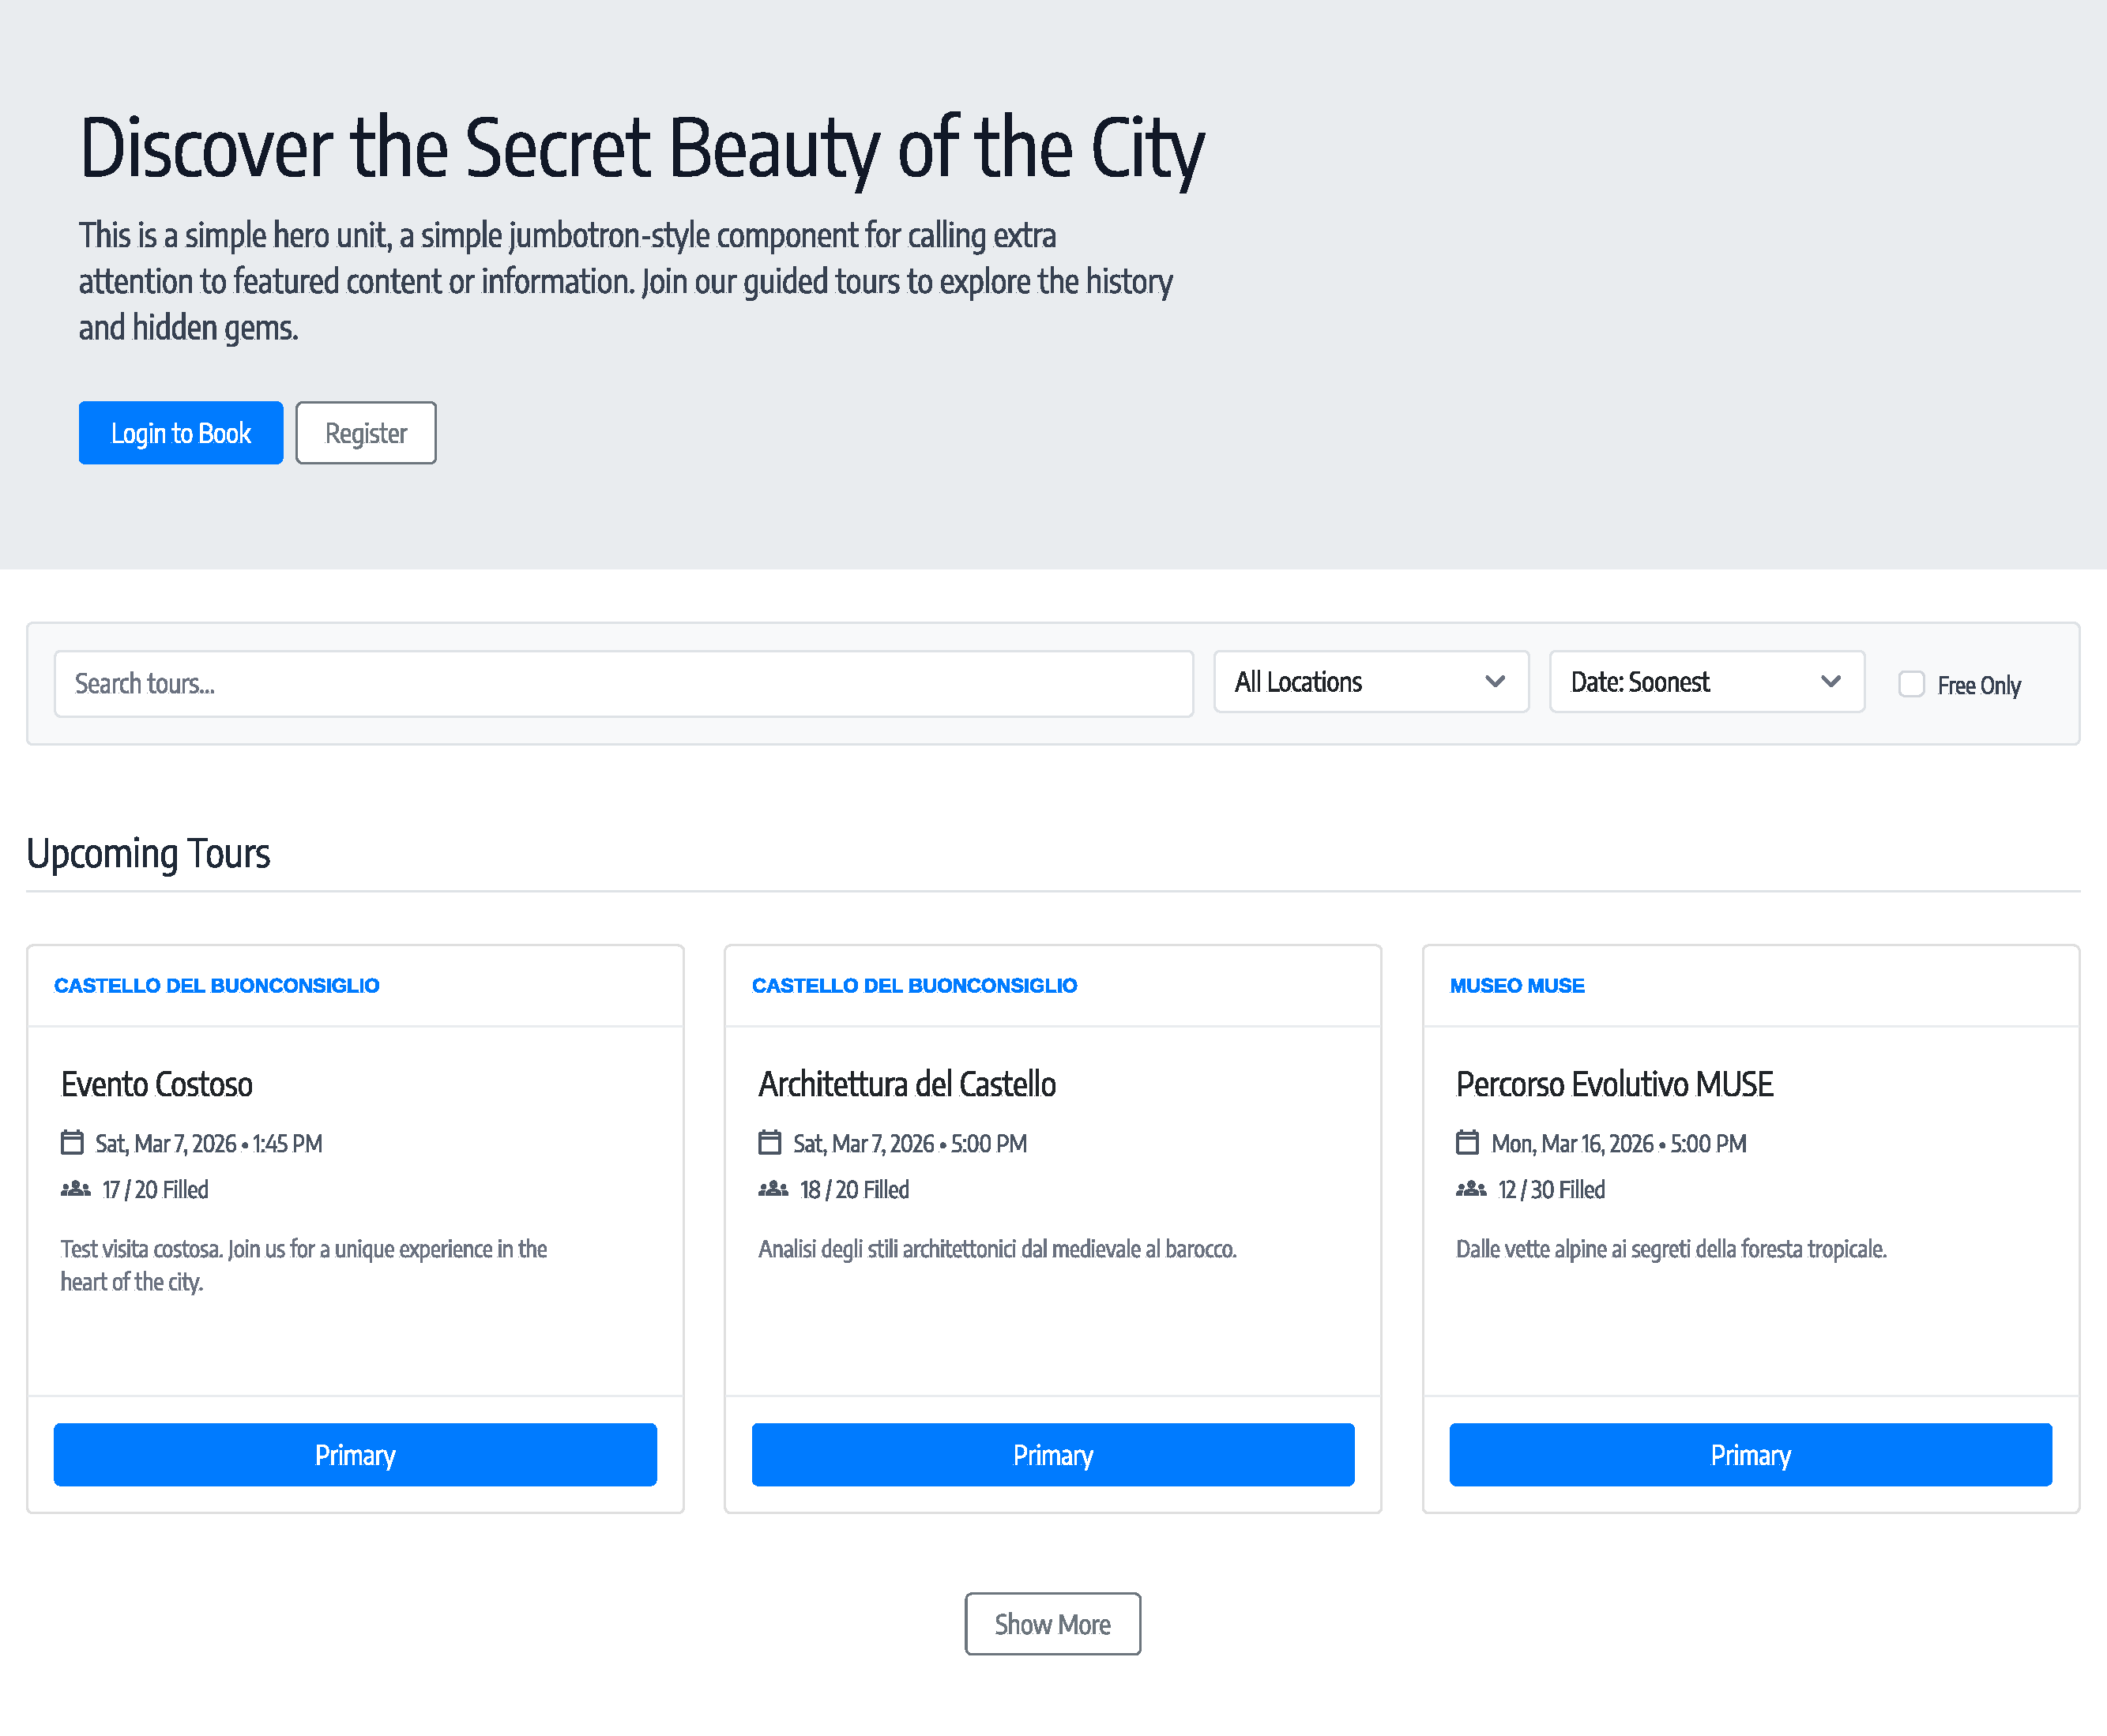
\includegraphics[width=0.9\textwidth, keepaspectratio]{capitoli/immagini/mockup/home.pdf}
    \caption{Mock-up della Home Page: il catalogo dei tour è presentato tramite card uniformi con immagine, titolo, luogo, data, posti residui e badge di stato. I filtri di ricerca (testo, distanza, gratuità) e l'ordinamento sono esposti in linea sopra la griglia, abbattendo il carico cognitivo necessario per individuare un tour di interesse.}
    \label{fig:mockup_home}
\end{figure}

% ── Mockup: Registrazione Visita ─────────────────────────────────────────────
\begin{figure}[H]
    \centering
    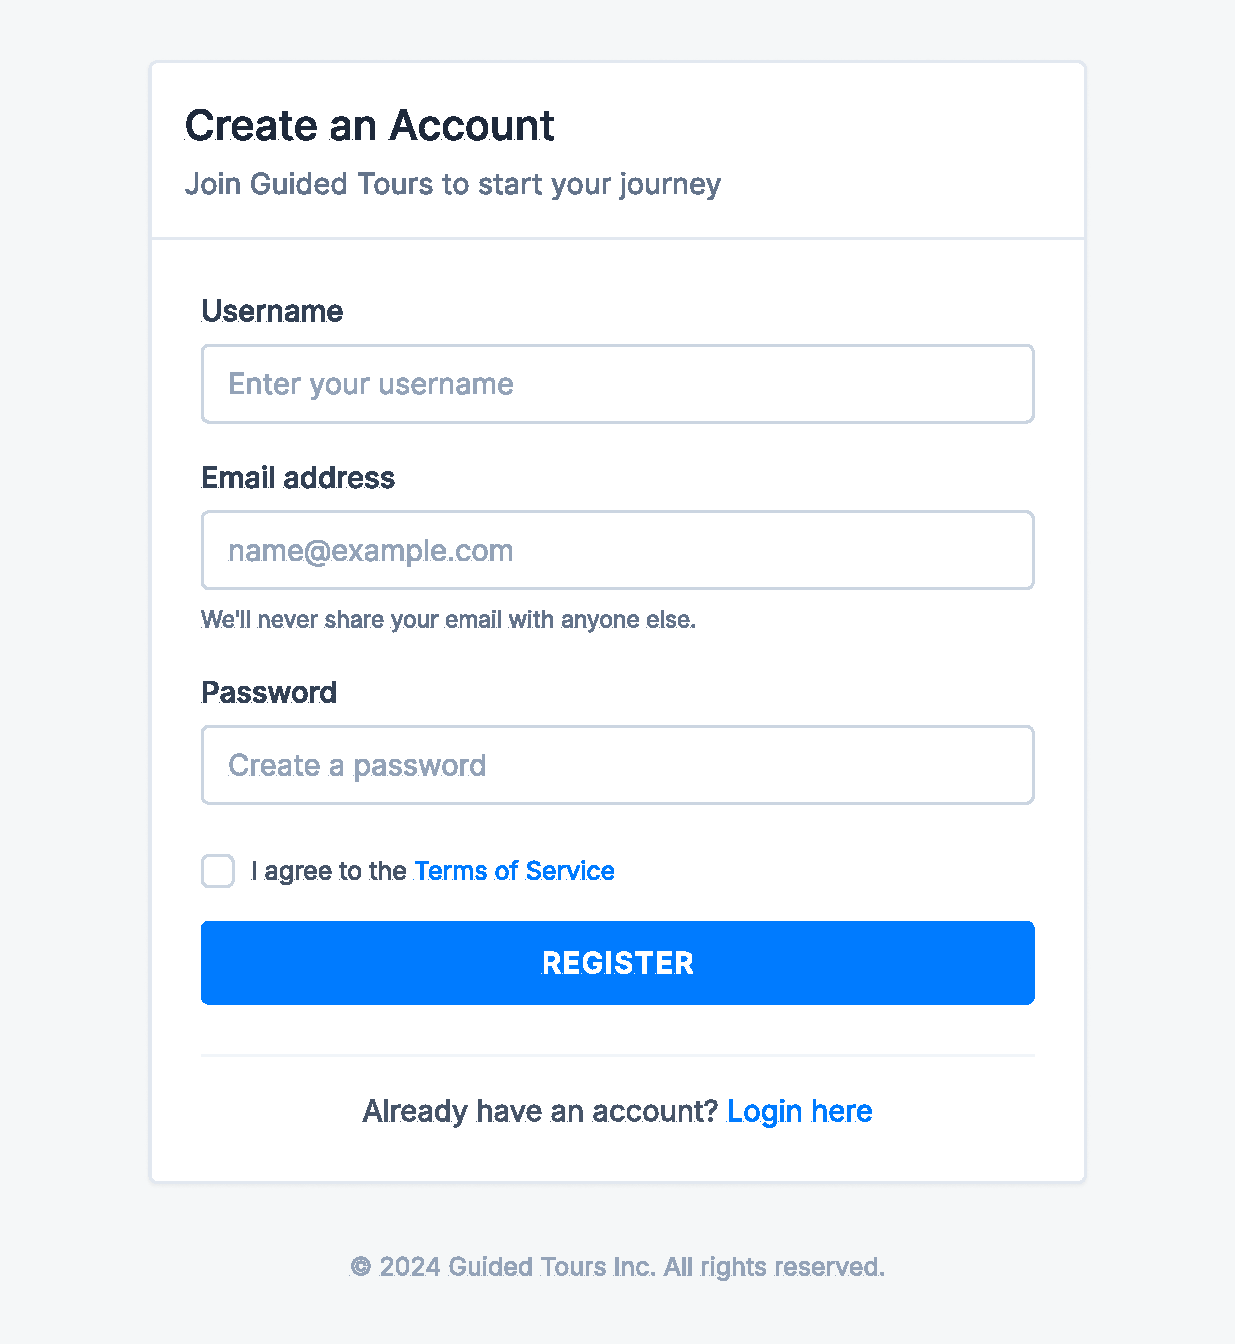
\includegraphics[width=0.75\textwidth, keepaspectratio]{capitoli/immagini/mockup/register.pdf}
    \caption{Mock-up della schermata di prenotazione visita: il modulo riepilogativo mostra il dettaglio del tour selezionato (luogo, data, prezzo, posti disponibili) affiancato al campo di selezione del numero di partecipanti. Il feedback sui vincoli (scadenza prenotazione, posti rimasti) è esposto in linea, in anticipo rispetto all'invio del form.}
    \label{fig:mockup_register}
\end{figure}

% ── Mockup: Dashboard Fruitore ───────────────────────────────────────────────
\begin{figure}[H]
    \centering
    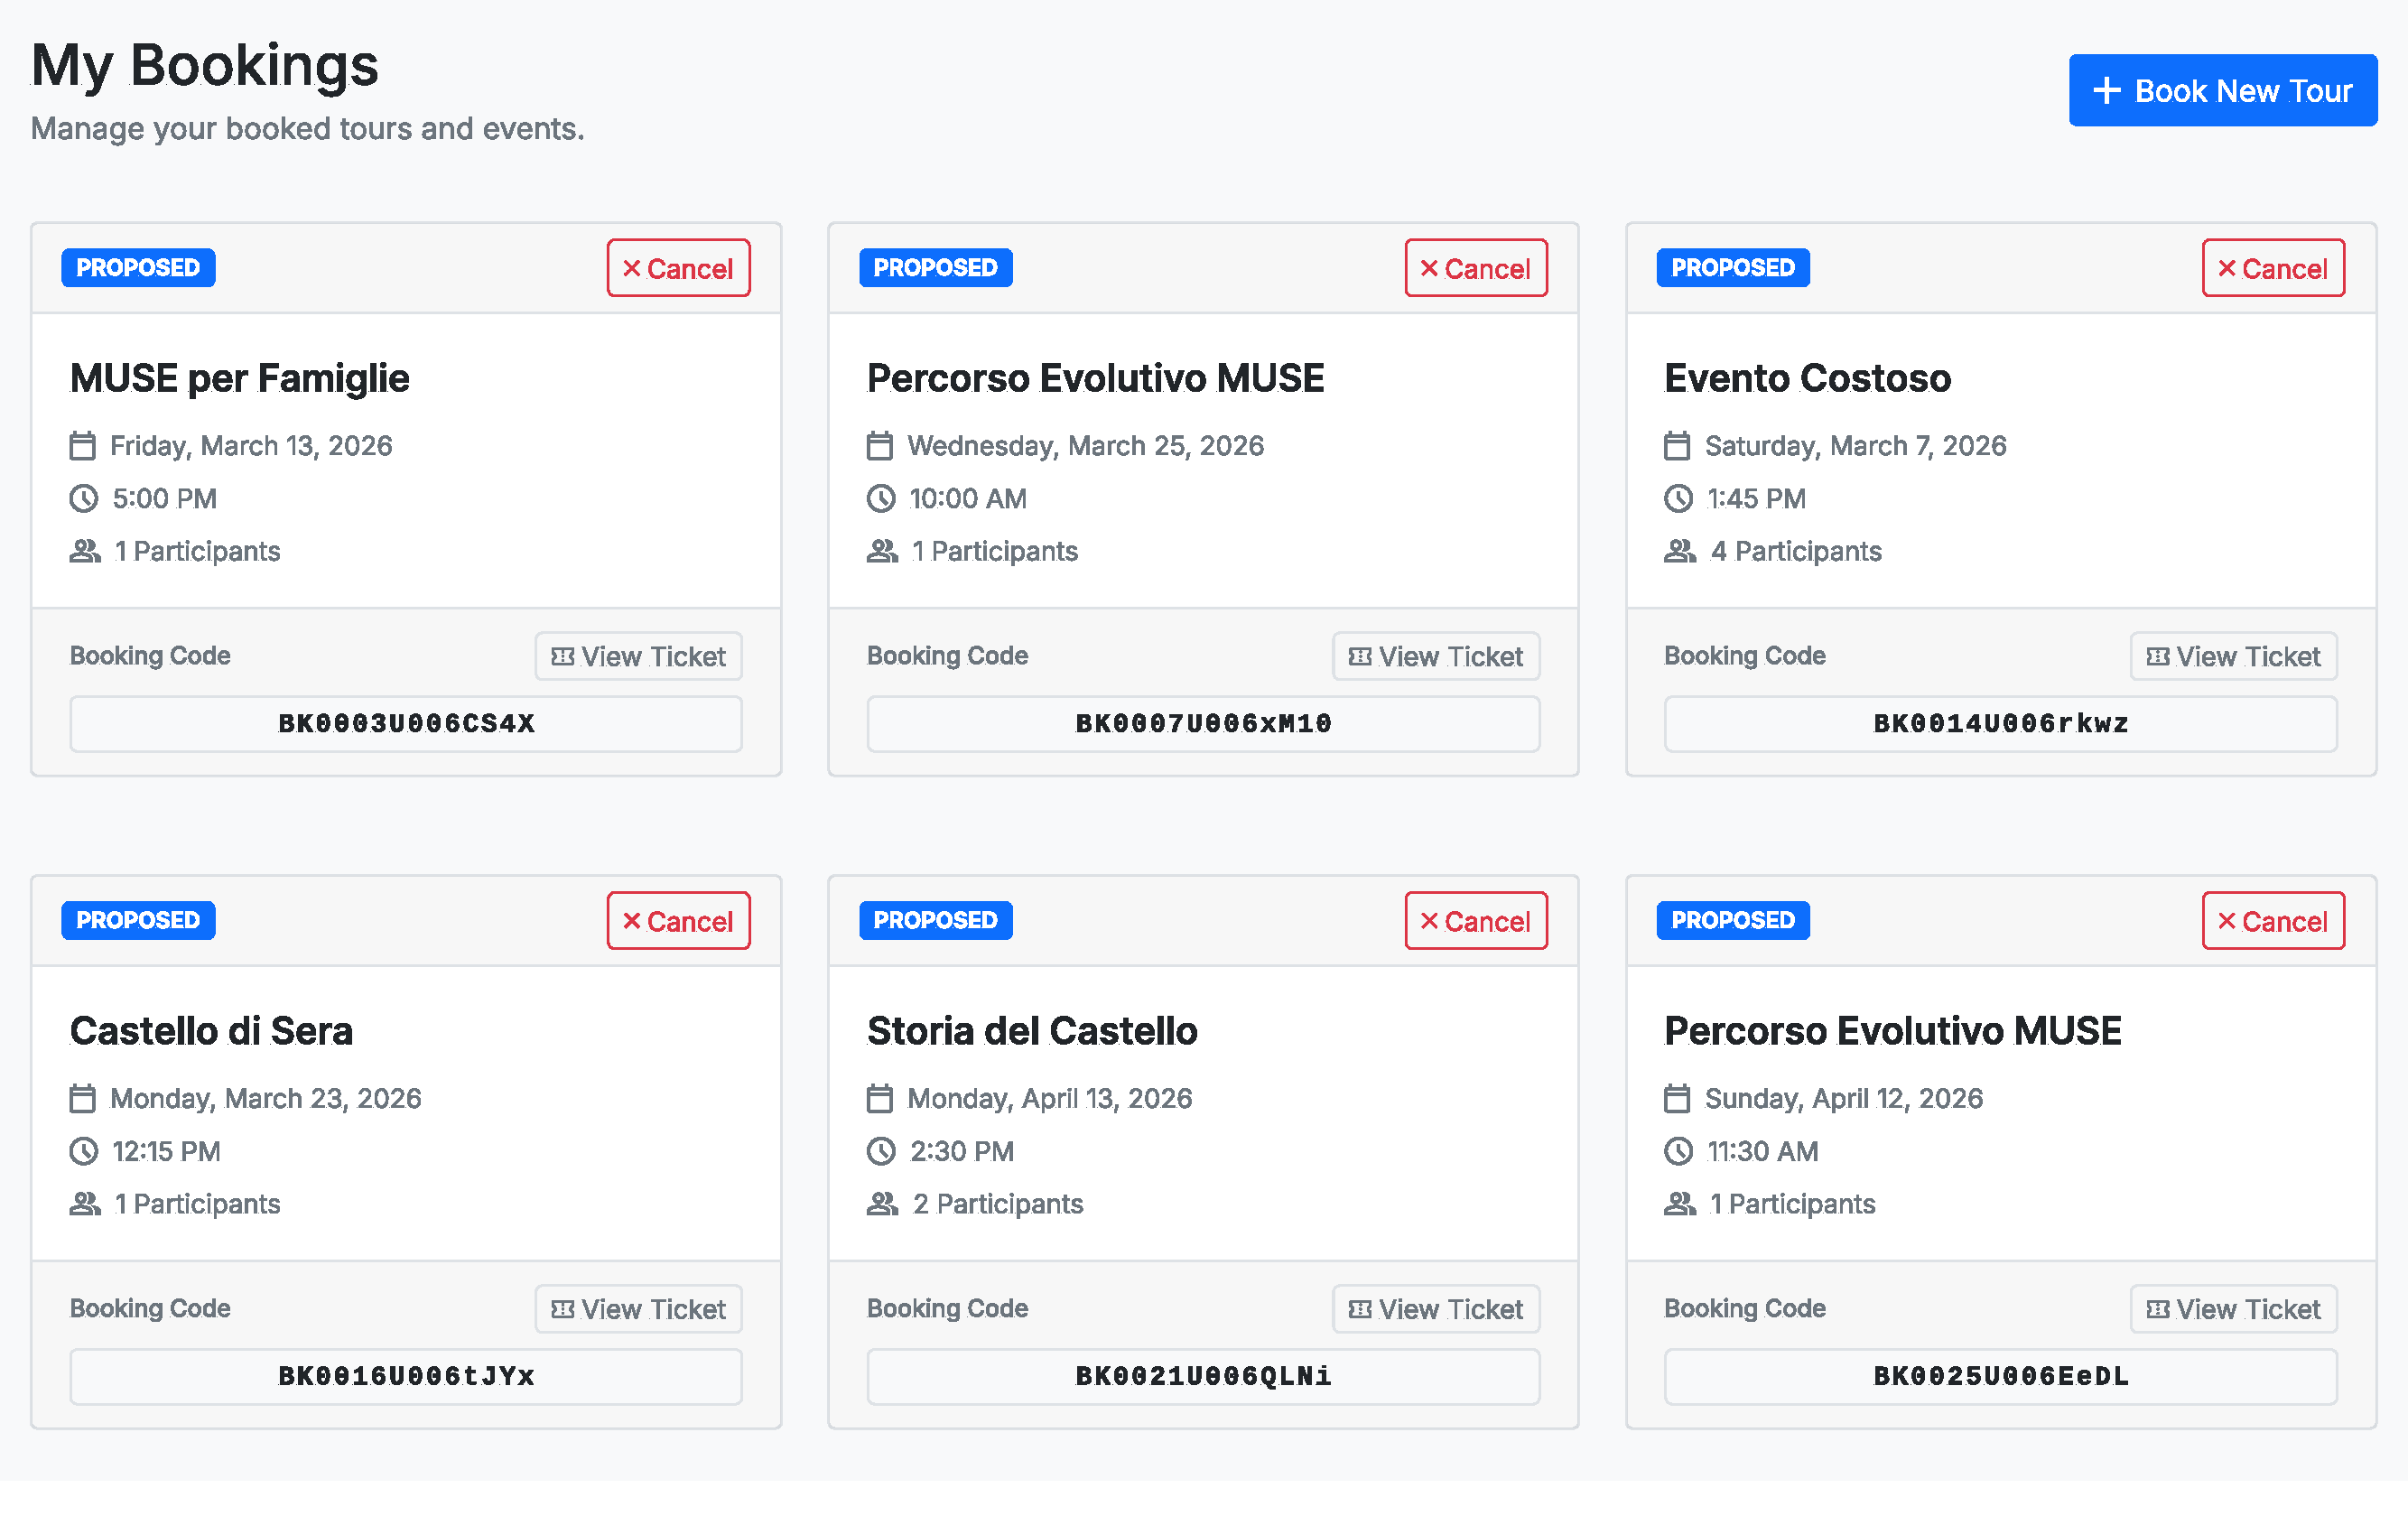
\includegraphics[width=0.9\textwidth, keepaspectratio]{capitoli/immagini/mockup/user-booking.pdf}
    \caption{Mock-up della dashboard del Fruitore — sezione prenotazioni attive: ogni prenotazione è presentata in una card che riporta il codice di prenotazione in font monospaziato, il numero di partecipanti, lo stato della visita e il pulsante di cancellazione con modale di conferma, risolvendo le problematiche di affordance e visibilità emerse nell'analisi euristica (P22, P24, P25).}
    \label{fig:mockup_user_booking}
\end{figure}

\begin{figure}[H]
    \centering
    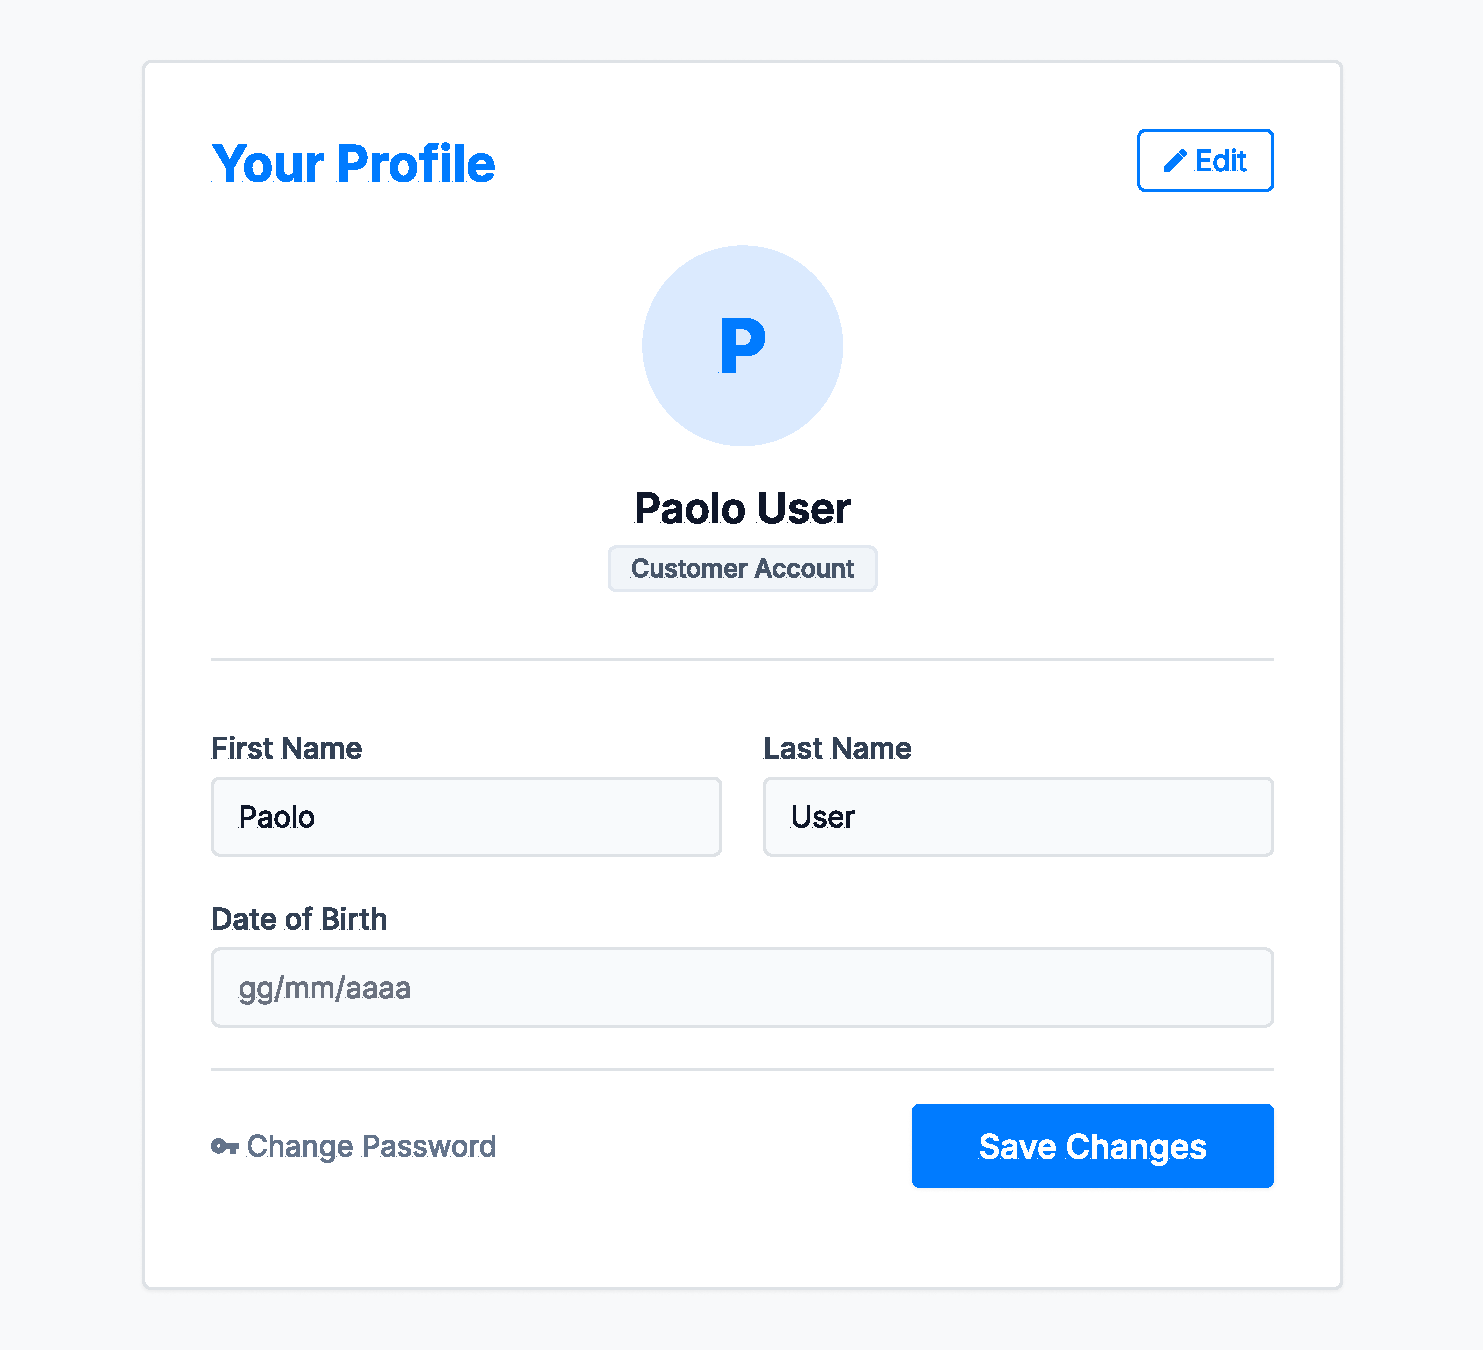
\includegraphics[width=0.75\textwidth, keepaspectratio]{capitoli/immagini/mockup/user-profile.pdf}
    \caption{Mock-up della sezione profilo utente: il pannello consente la modifica dei dati anagrafici e il cambio password direttamente dall'area personale, con validazione live dei campi e feedback semantico immediato sullo stato del salvataggio.}
    \label{fig:mockup_user_profile}
\end{figure}

% ── Mockup: Pannello Guide ───────────────────────────────────────────────────
\begin{figure}[H]
    \centering
    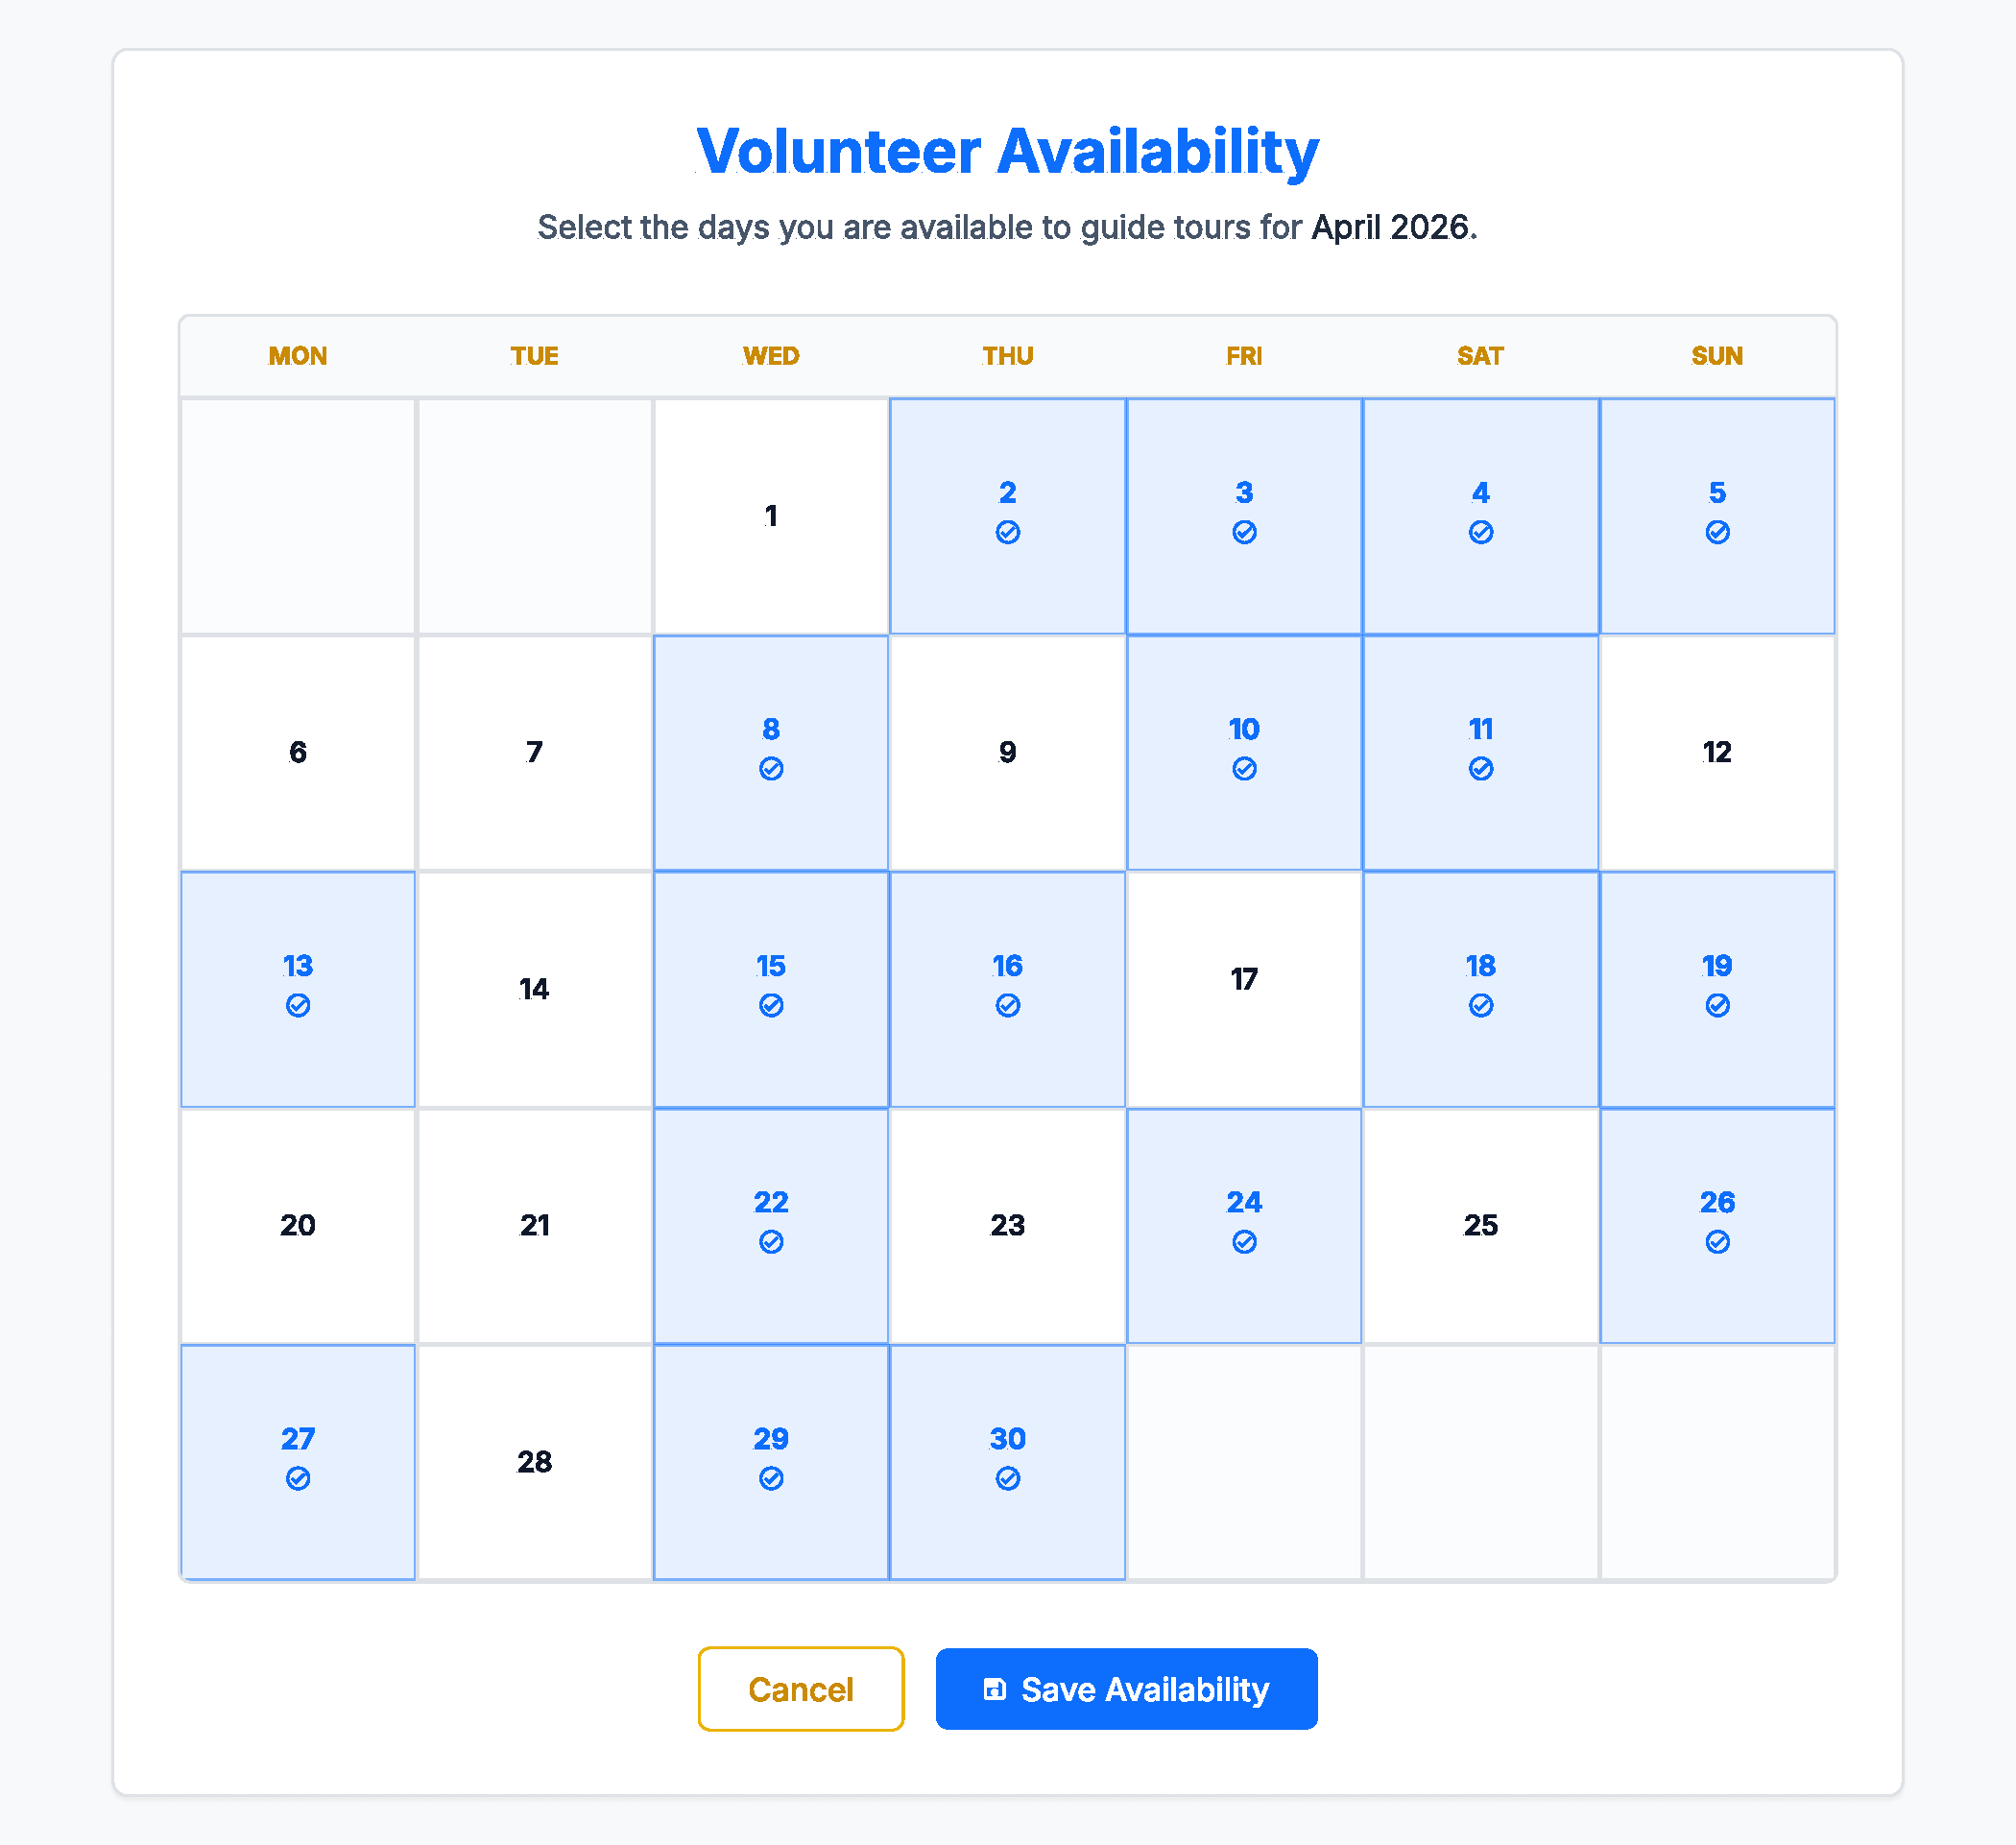
\includegraphics[width=0.9\textwidth, keepaspectratio]{capitoli/immagini/mockup/vol-availability.pdf}
    \caption{Mock-up del calendario disponibilità della Guida: la vista mensile a griglia permette di selezionare singole date o intere colonne (giorni della settimana) con un solo click, riducendo il numero di interazioni necessarie per dichiarare disponibilità ricorrenti (es. ogni sabato del mese).}
    \label{fig:mockup_vol_availability}
\end{figure}

\begin{figure}[H]
    \centering
    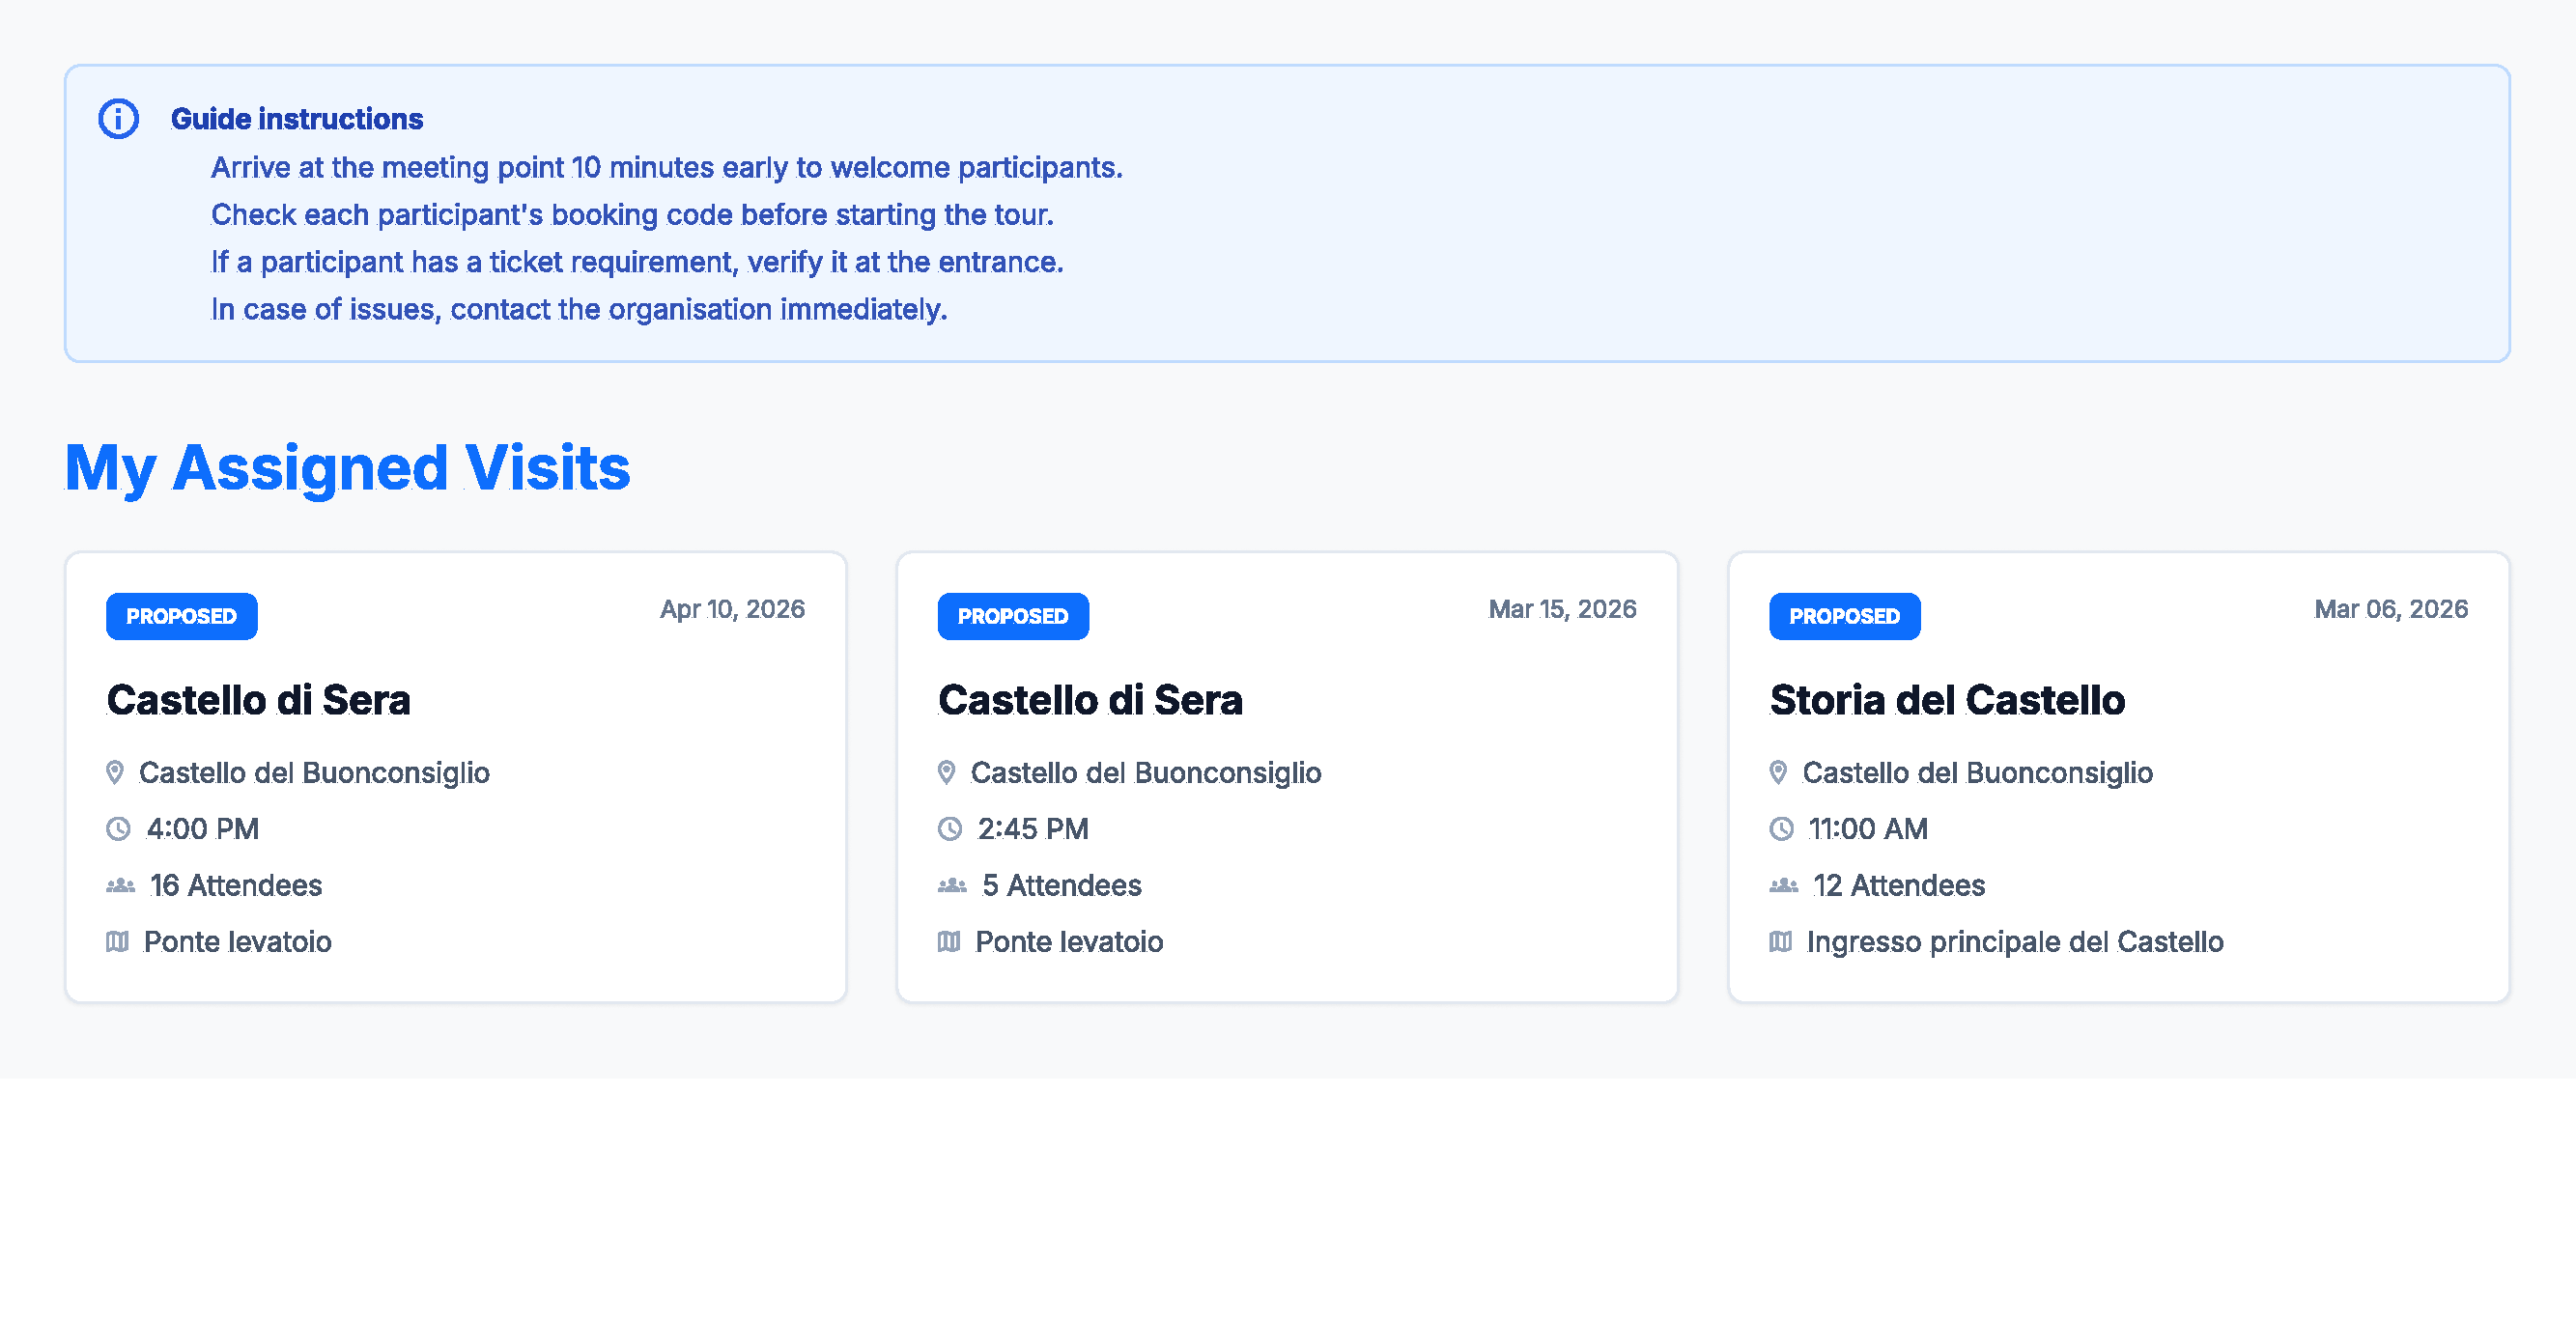
\includegraphics[width=0.9\textwidth, keepaspectratio]{capitoli/immagini/mockup/vol-panel.pdf}
    \caption{Mock-up del pannello visite assegnate alla Guida: la lista cronologica delle visite in programma espone data, luogo, numero di iscritti e stato, affiancata da un riquadro informativo con le istruzioni operative (verifica biglietti, gestione partecipanti), rispondendo alla problematica P37 relativa all'assenza di indicazioni operative contestuali.}
    \label{fig:mockup_vol_panel}
\end{figure}

% ── Mockup: Pannello Amministratore ─────────────────────────────────────────
\begin{figure}[H]
    \centering
    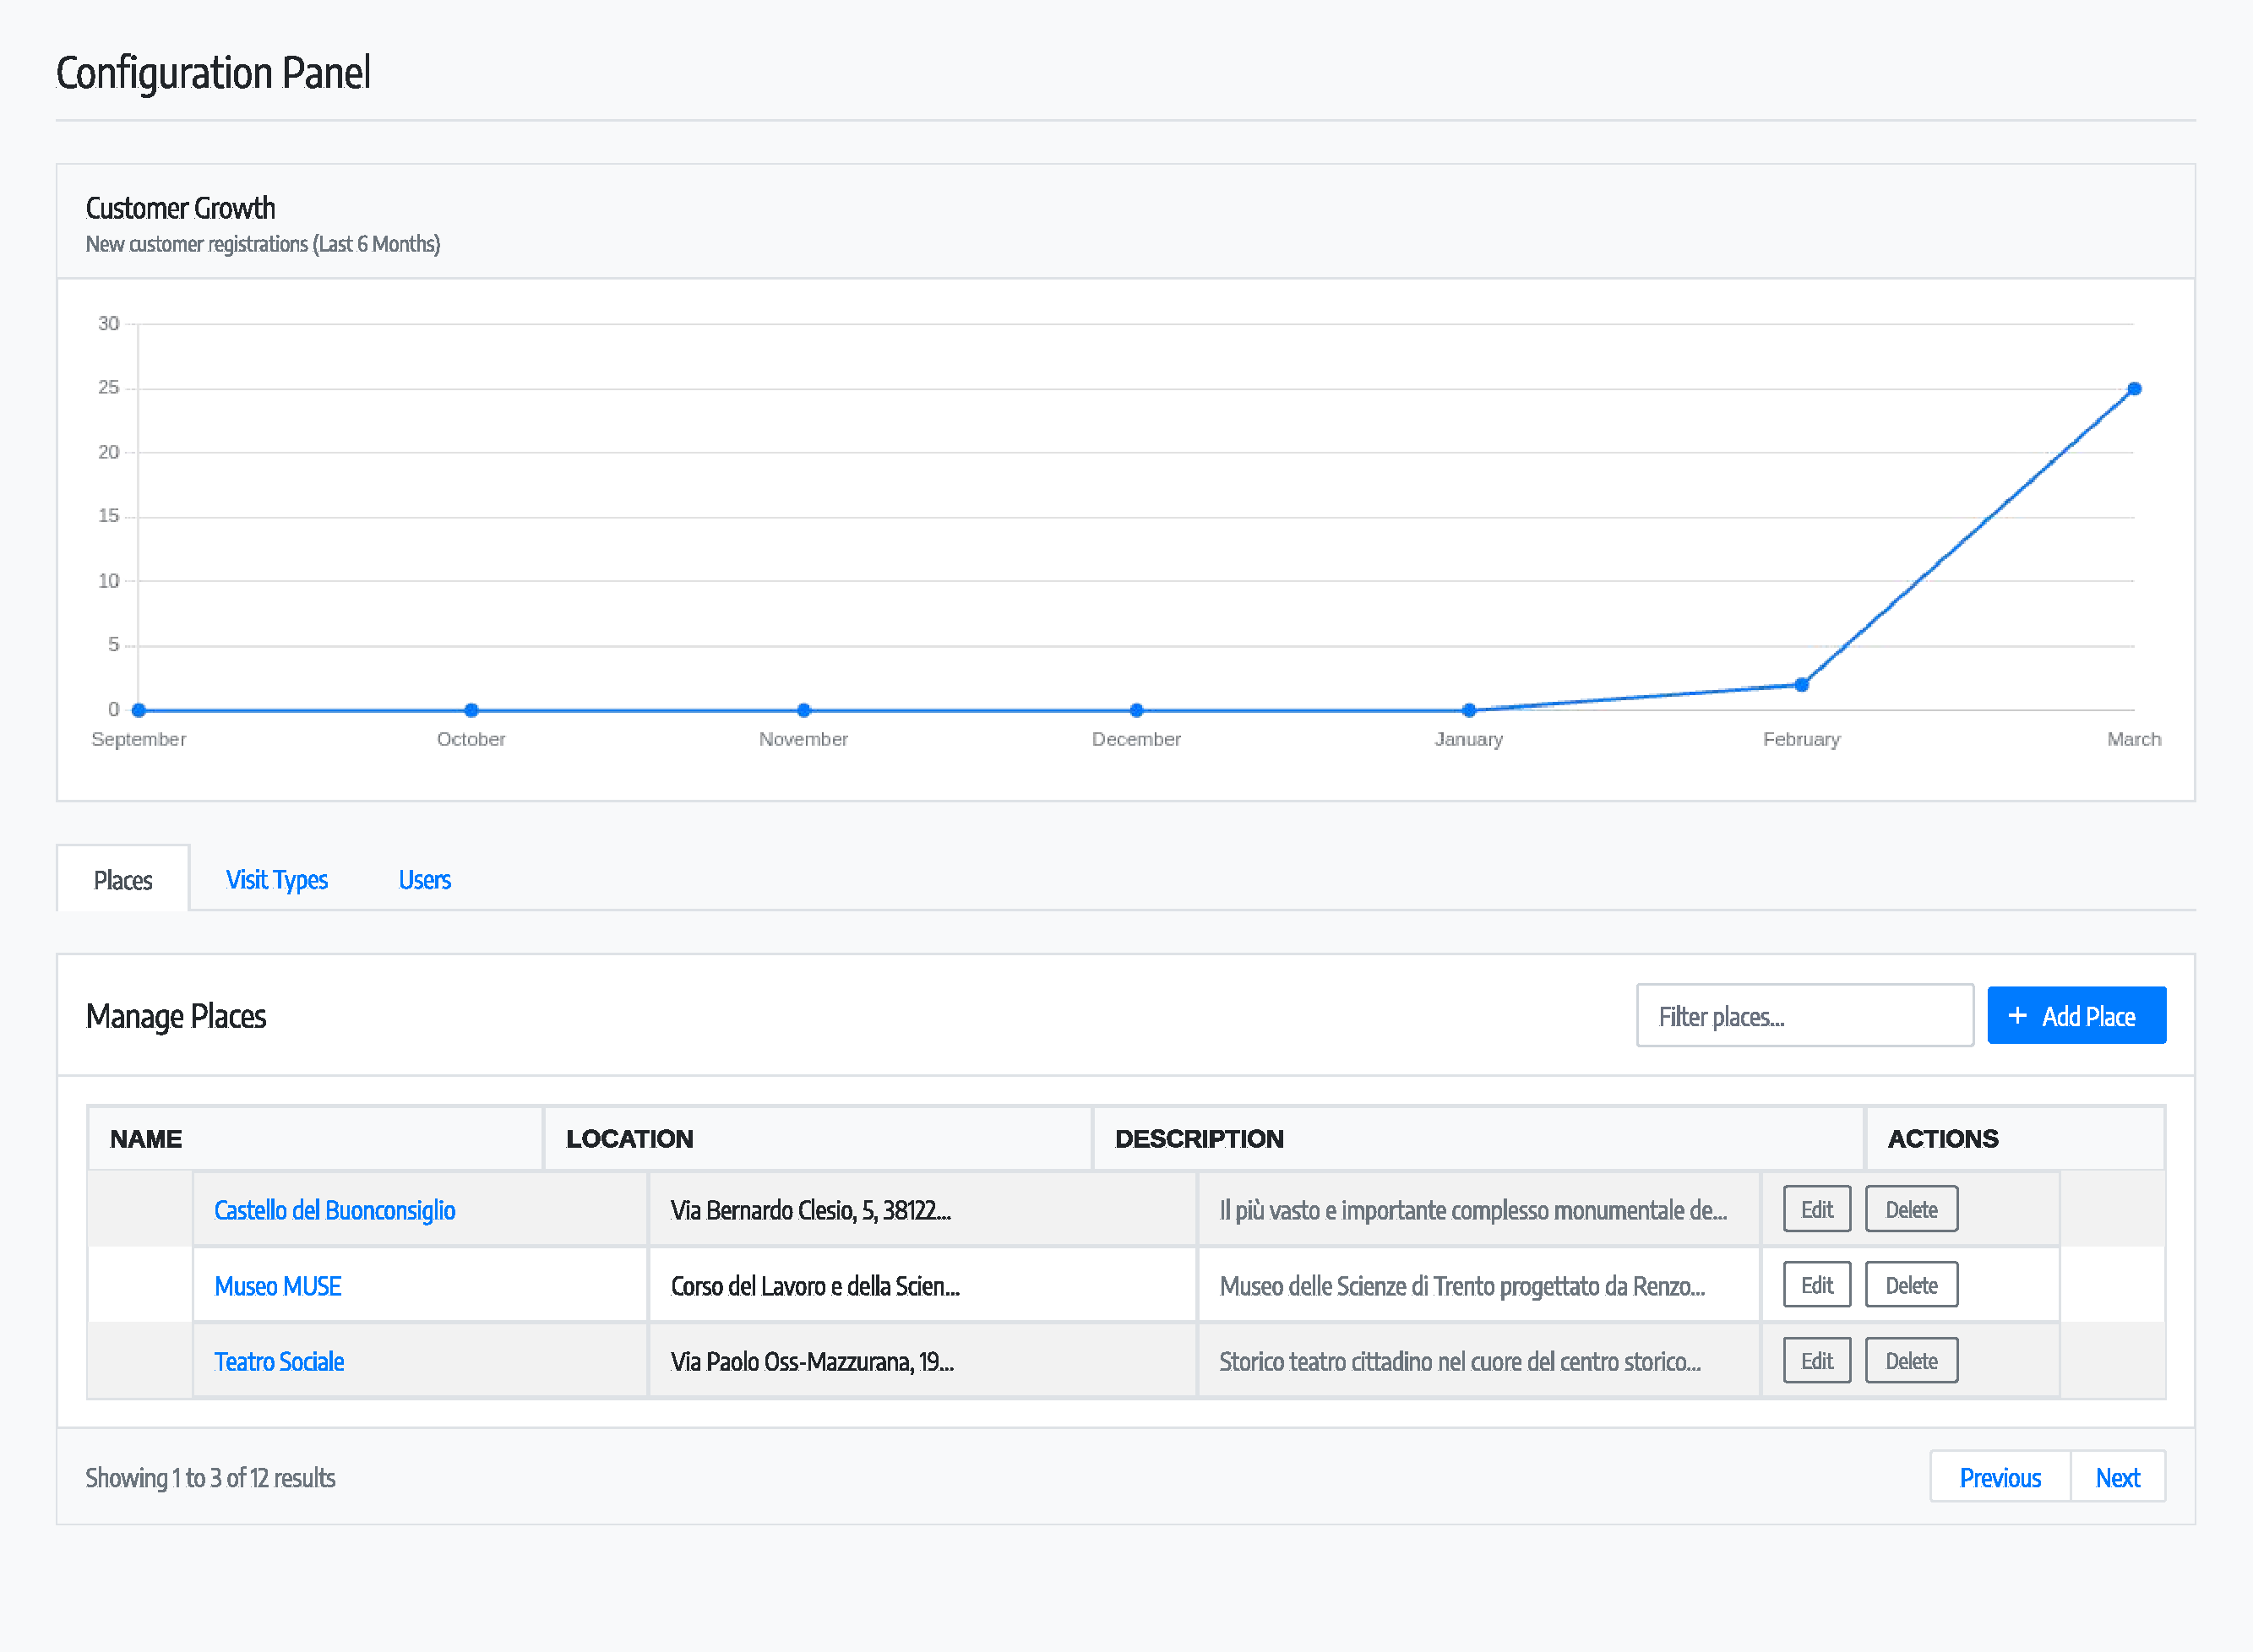
\includegraphics[width=0.9\textwidth, keepaspectratio]{capitoli/immagini/mockup/config-panel.pdf}
    \caption{Mock-up del pannello di configurazione amministratore: la sezione centralizza la gestione di utenti, luoghi e tipologie di visita in tab distinte. Il modale di eliminazione con richiesta di conferma esplicita risolve la problematica P29 (assenza di guardia prima della cancellazione), mentre la validazione in tempo reale dei campi password risponde alla problematica P28.}
    \label{fig:mockup_config_panel}
\end{figure}

\begin{figure}[H]
    \centering
    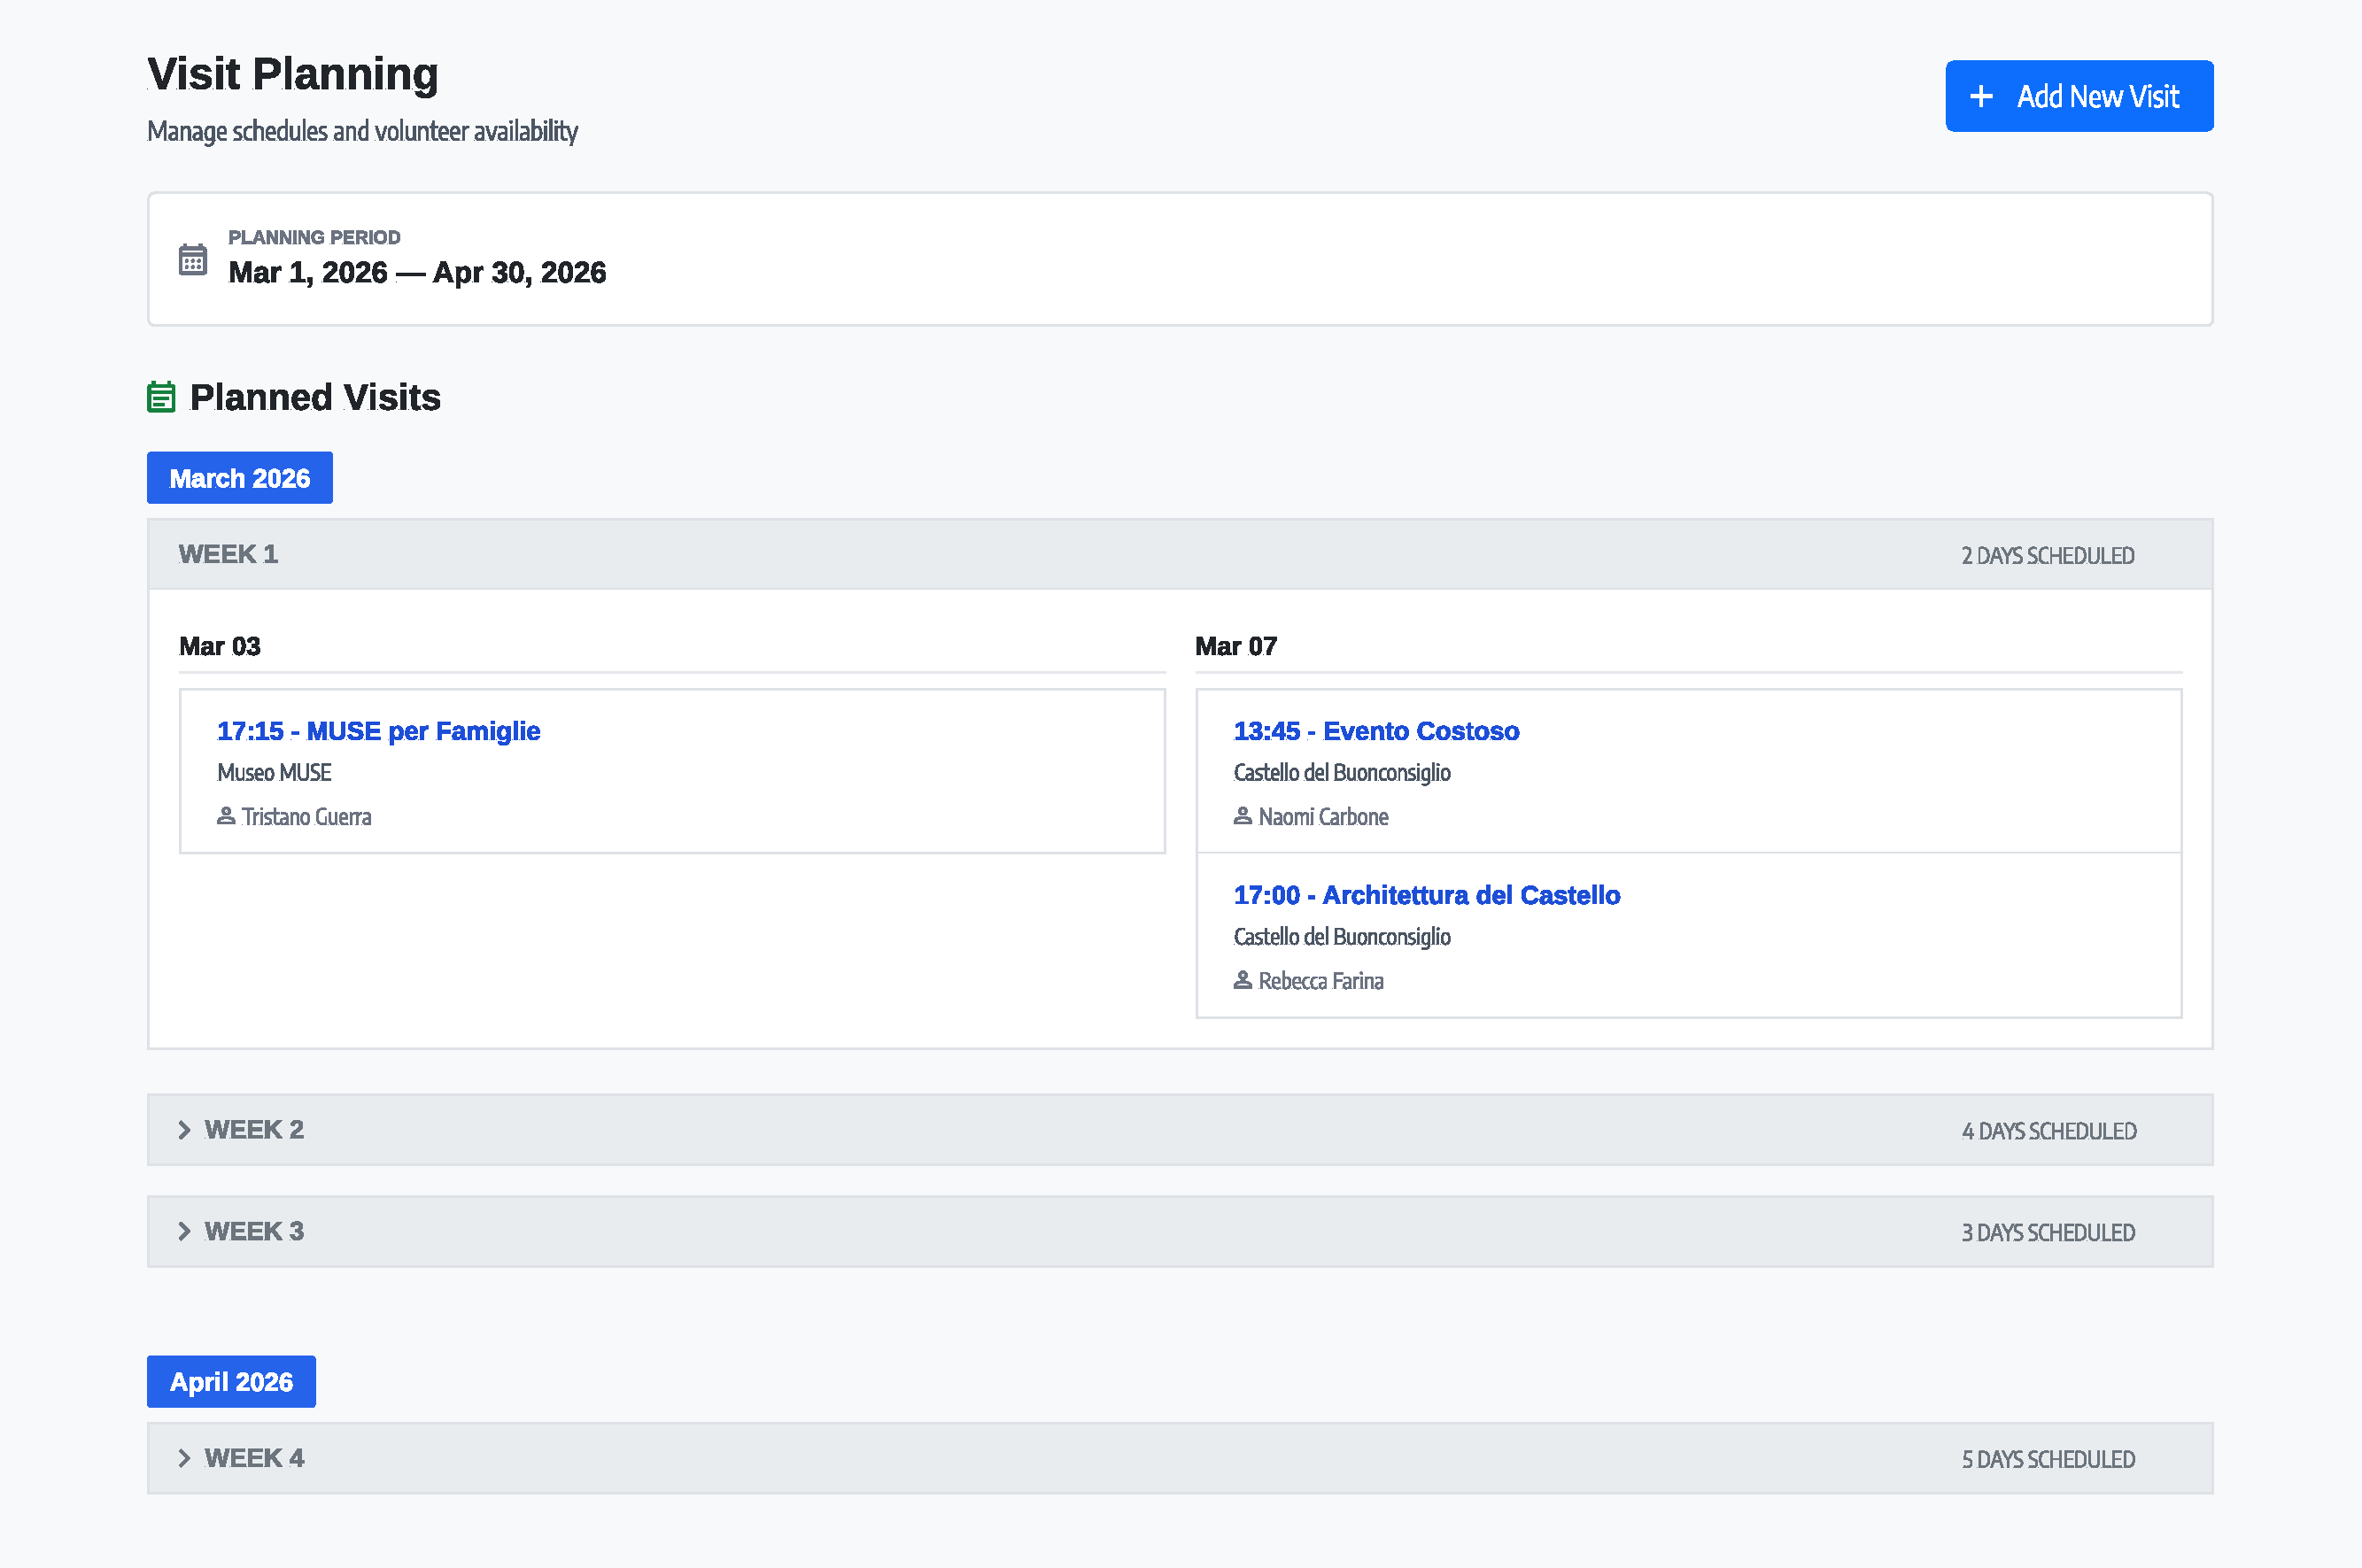
\includegraphics[width=0.9\textwidth, keepaspectratio]{capitoli/immagini/mockup/config-planning.pdf}
    \caption{Mock-up del pannello di pianificazione visite (Visit Planning): le visite sono raggruppate cronologicamente per mese e settimana, con evidenziazione cromatica dello stato (proposta, confermata, effettuata). Il flusso guidato di creazione visita — selezione tipo, data, guida disponibile — è accessibile tramite un unico pulsante contestuale, risolvendo la disorganizzazione del layout segnalata in P30 e P31.}
    \label{fig:mockup_config_planning}
\end{figure}

\subsection{Validazione Formativa dei Prototipi (Mock-up)}
Prima di procedere alla stesura del codice (coding), i mock-up ad alta fedeltà realizzati su Figma sono stati sottoposti a un meticoloso processo di validazione formativa. Il team ha adottato un approccio metodologico ibrido, diviso in due macro-fasi sequenziali, al fine di ottimizzare preventivamente l'esperienza utente.

La prima fase, di natura interna (Esperti), è consistita in un'ispezione analitica da parte del team di sviluppo. Avvalendosi del metodo del \textit{Cognitive Walkthrough}, i progettisti hanno navigato i prototipi validando la coerenza dei flussi logici (\textit{User Flows}) interattivi e verificando accuratamente il corretto posizionamento delle \textit{affordance}.

La seconda fase, di carattere esterno (Utenti finali), ha coinvolto un campione empirico ristretto di 3 individui estranei al progetto. Aderendo ai moderni dettami metodologici della \textit{Lean UX} e del \textit{Guerrilla Testing}, si è optato per una valutazione qualitativa snella. Ai partecipanti è stato chiesto di interagire liberamente con il prototipo, verbalizzando i propri ragionamenti ad alta voce secondo il celebre protocollo \textit{Think-Aloud}. La decisione di affidarsi a soli tre utenti trova solida giustificazione negli studi accademici di Jakob Nielsen, i quali dimostrano empiricamente che un campione da 3 a 5 soggetti è ampiamente sufficiente per far emergere la stragrande maggioranza delle criticità euristiche.

Questo collaudo formativo ha permesso di correggere la rotta progettuale prima di impegnare risorse nello sviluppo software (coding), demandando la misurazione statistica e oggettiva all'esperimento sommativo finale.

\section{Technical Rationale}
La risoluzione delle criticità di usabilità ha richiesto un intervento sia lato Front-end che lato Back-end. Di seguito i principali interventi tecnologici:
\begin{itemize}
    \item \textbf{Gestione del Design System}: Sebbene alcune opzioni progettuali potessero far pensare a Tailwind CSS, l'interfaccia finale è stata uniformata sfruttando appieno il framework \textbf{Bootstrap 5} unitamente a variabili SCSS customizzate (\texttt{\_variables.scss} e \texttt{app.scss}). Questo ha permesso di mantenere pulita la gerarchia del codice CSS, impiegando classi di utilità in modo mirato unicamente dove necessario.
    \item \textbf{Validazione e Feedback in tempo reale}: Il sistema sfrutta la \textbf{validazione integrata di Laravel} (tramite \texttt{\$request->validate()}) all'interno dei Controller (es. \texttt{UserController}, \texttt{AdminController}) per assicurare la robustezza dei dati. A livello di interfaccia frontale, script in \textit{Vanilla JavaScript} gestiscono messaggi di validazione live (come i controlli sulla robustezza della password nel configuratore), fornendo all'utente un feedback immediato già in fase di digitazione.
    \item \textbf{Meccanismi di conferma (Modal)}: I \textit{confirmation modals} per le azioni distruttive, al posto di impiegare librerie più pesanti come Livewire, sono stati realizzati tramite \textbf{Modali Bootstrap} nativi interfacciati con script JavaScript centralizzati. Questo rende più performante la pagina: uno script globale cattura l'evento, estrae dinamicamente i parametri utente/oggetto (\texttt{data-action}, \texttt{data-item-name}) e inserisce i dati prima della visualizzazione del modale, garantendo modularità.
\end{itemize}

\section{Reverse Engineering e Documentazione del Visual Design dal Codice}
Il restyling grafico ha posto forte enfasi sull'accessibilità, cercando di risolverne un difetto di base emerso nell'analisi. Attraverso il \textit{reverse engineering} dei fogli di stile customizzati (file \texttt{\_variables.scss} e \texttt{app.scss}) e dei template base dell'interfaccia (es. \texttt{app.blade.php}), è possibile mappare formalmente i principi di visual design adottati nel sistema.

\subsection{Psicologia e Gerarchia del Colore}
La palette cromatica estratta dal codice definisce una gerarchia visiva basata su un forte contrasto, progettata per bilanciare l'aderenza all'estetica istituzionale con l'usabilità:
\begin{itemize}
    \item \textbf{Primario (Vibrant Blue, \#0d6efd):} Impiegato per le azioni principali (\textit{call-to-action}) e le direttive di navigazione primaria. Comunica sicurezza e grande affidabilità professionale.
    \item \textbf{Secondario e Accento (Amber/Gold, \#ffc107):} Riservato per le notifiche di avviso (\textit{warning}) o per polarizzare focalmente l'attenzione visuale in contesti con alta densità informativa.
    \item \textbf{Feedback Semantico (Success \#198754, Danger \#dc3545, Info \#0dcaf0):} Il frontend sfrutta sistematicamente questa sintassi cromatica universale per i \textit{Live Input Feedback} (es. form validation) e per marcare le alterazioni critiche dello stato (es. i \textit{Global Delete Modal} in rosso), abbattendo i tempi di ricezione cognitiva degli esiti di sistema.
    \item \textbf{Colori Neutri e Tema Scuro:} Le variabili architetturali \texttt{--bs-body-bg} (\#121212) e \texttt{--card-bg} (\#2a2a2a) presenti nel blocco nativo del tema \textit{dark} dimostrano una stratificazione atta a sopprimere l'affaticamento oculare (\textit{eye-strain}). Viene adoperato un grigio antracite al posto del nero assoluto, esaltando otticamente il volume del componente sollevato rispetto al fondale. Vi si accavallano filtri traslucidi (\textit{glassmorphism} settato all'85\% di opacità, es. \texttt{rgba(42, 42, 42, 0.85)}) che permettono ai layer di compenetrarsi organicamente.
\end{itemize}

\subsection{Tipografia e Leggibilità}
Dall'ispezione della dichiarazione centrale globale (\texttt{\$font-family-sans-serif}), emerge primariamente l'utilizzo dell'innovativa famiglia tipografica \textit{Outfit} (importata via \textit{Google Fonts}) e del successivo \textit{system stack}. Si tratta di un \textit{sans-serif} geometrico assai limpido, leggibile a qualsivoglia scalatura *viewport*.

La gerarchia dei pesi è decisa sincreticamente all'adozione delle utility del framework (\texttt{display-4}, \texttt{h3}, \texttt{h5}), abbinate per la titolazione ad un peso netto e consistente (\texttt{\$headings-font-weight: 600;}). Scelte del genere irrobustiscono e incanalano efficacemente lo \textit{scanning pattern} oculare rapido (stile F-Pattern), demarcando con solida incisività il perimetro visivo della \textit{hero section} dai normali blocchi testuali più analitici di un \textit{body} classico.

\subsection{Spaziature e Principi della Gestalt}
Le logiche strutturali CSS di \textit{Guided Tours} e i costrutti formali del layout adottati traslano in codice i fondamenti pervasivi dettati dalla psicologia della forma (\textit{Gestalt}):
\begin{itemize}
    \item \textbf{Prossimità e Regione Comune:} L'impiego pervasivo di \texttt{.card} dotate di raggiature accentuate (\texttt{border-radius: 1rem}) unito a background cromaticamente scissi (\texttt{--card-bg}), delimita materialmente insiemi eterogenei in una sola "regione comune" raggruppata logicamente. La separazione visiva è amministrata da una netta abbondanza di padding regolari (\texttt{py-5}, \texttt{gap-2}) che disaccoppia entità estranee alleggerendone drasticamente la tensione di decifrazione (\textit{Legge della Prossimità}).
    \item \textbf{Feedback Tattile Implicito (Buona Continuazione):} Le tessere (\textit{Cards}) accolgono micro-transizioni reattive (\texttt{.card-hover:hover}) che traducono un istantaneo vettore verticale di elevazione (\texttt{translateY(-8px)}), associato ad intensificazione dell'ombra (\textit{drop-shadow}). Tali riscontri tridimensionali emulano solide affordance del mondo fisico, canalizzando per implicita continuazione visiva le scelte esplorative e il rassicurante cliccaggio dei dispositivi di input dell'internauta.
\end{itemize}

\section{Design Pattern d'Interazione (HCI)}
L'interfaccia è stata costruita assemblando diversi Design Pattern consolidati nella Human-Computer Interaction, al fine di garantire familiarità, ridurre il carico cognitivo e accelerare la curva di apprendimento per i diversi profili utente presenti nel vario panorama del progetto:
\begin{itemize}
    \item \textbf{Cards (Schede Visive)}: Impiegate massicciamente nella \textit{Home Page} per raggruppare coerentemente i metadati di ogni singolo tour (titolo, data, luogo, posti disponibili). Questo pattern astrae la complessità del database in blocchi visivi scansionabili e logicamente isolati, ideali per la fruizione mobile e per l'immediatezza cognitiva.
    \item \textbf{Navigation Tabs (Pannelli a schede)}: All'interno dell'area \textit{Admin Configurator}, la gestione di "Places", "Visit Types" e "Users" è organizzata in sezioni a tabulazione. Ciò elimina il \textit{page refresh} continuo e compatta le opzioni amministrative critiche in un'unica plancia, ottemperando all'euristica del design estetico minimalista senza eccessivo rumore visivo.
    \item \textbf{Global Navigation Bar (Menu Persistente)}: Una barra di navigazione fissa posta al vertice funge da àncora di salvataggio e di orientamento perpetuo per l'utente. Rende costantemente accessibili i link operativi determinanti (Home, Accesso, o Dashboard personale) prescindendo dal grado di scorrimento verticale.
    \item \textbf{Faceted Search \& Filter Bar}: Pattern primario inserito nella \textit{Home Page} a favore del \textit{Fruitore}. Permette di modulare dinamicamente i risultati (filtro per luogo, stringa testuale, ordine temporale o scrematura dei costi), snellendo il tempo di scoperta e trasmettendo il senso di controllo e libertà d'azione.
    \item \textbf{Visual Status Badges (Codifica semantica a etichette)}: Guidato dalla nuova palette cromatica del sistema, l'impiego di tag "pill" compatti (come "Open", "Imminent" per le visite, oppure i tag dei ruoli amministrativi) restituisce una profilazione visiva in una frazione di secondo. Alimenta il principio di \textit{recognition rather than recall}.
    \item \textbf{Confirmation Trigger (Modali antierrore distruttivo)}: Al fine di prevenire errori di esecuzione involontari (\textit{slips}) durante le operazioni di Backoffice (es. l'annullamento di risorse storicizzate o la rimozione di un volontario), è stato introdotto un meccanismo di controllo preventivo. L'interfaccia intercetta l'azione distruttiva attraverso un "Global Delete Modal", costringendo così l'utente a validare l'azione in modo esplicito e consapevole ("This action cannot be undone").
    \item \textbf{Continuous / Asynchronous Scrolling (Load More)}: Rispetto a un'impaginazione classica tradizionale, che potrebbe frammentare l'esplorazione, l'utilizzo di un pattern asincrono incrementale per l'elenco dei tour consente una navigazione progressiva nel catalogo, mantenendo sempre visibili e accessibili l'header e il form dei filtri.
    \item \textbf{Live Input Feedback (Validazione Contestuale)}: Questo pattern è implementato nei form critici per comunicare istantaneamente il rispetto o la violazione dei vincoli strutturali (es. i requisiti di robustezza della password). Fornendo un feedback in tempo reale, si riduce la frustrazione tipicamente associata agli errori di validazione notificati solo in fase di sottomissione (Submission Postponed Errors). 
\end{itemize}

\section{Role-Based Customization: Le 4 Home Page}
Per assecondare le diverse personas documentate in fase esplorativa, la Home Page (\texttt{home.blade.php}) agisce come smistatore univoco. Adatta infatti il suo layout e le proprie funzionalità in tempo reale basandosi sull'autenticazione tramite direttive di autorizzazione:
\begin{enumerate}
    \item \textbf{Guest (Visitatore Anonimo)}: Accolto da messaggi esplorativi con orientamento alla conversione, che invitano l'utente a registrarsi oppure a loggarsi ("Login to Book") per intraprendere un'esperienza guidata.
    \item \textbf{Customer (Fruitore)}: Visualizza pulsanti interattivi ("Browse Tours") per ispezionare istantaneamente il catalogo delle visite, unitamente ad uno shortcut persistente che rimanda alla "My Dashboard" per tenere d'occhio i biglietti.
    \item \textbf{Volunteer (Guida)}: Viene informato sin dalla prima riga a procedere all'interno della sua area specifica, al fine di impostare la propria personale disponibilità settimanale per l'abbinamento ai tour.
    \item \textbf{Admin (Configuratore)}: L'interfaccia muta in una plancia direzionale limitando le grafiche superflue; il testo guida l'amministratore e gli offre accesso rapido alla visualizzazione delle iscrizioni in aumento e alle statistiche base.
\end{enumerate}

\section{Feature Breakdown}

\subsection{Sistema di Filtering e Sorting dinamico}
Sulla Home Page pubblica, il pannello di ricerca esplorativo che correda la lista dei tour integra funzioni multiple: ricerca testuale live, filtro sulla località, vincolo sul costo ("Free Only") ed un selettore di ordinamento (temporale o alfabetico). Questa architettura è pilotata interamente in \textbf{Alpine.js}, che intercetta l'evento di sottomissione assemblando i parametri in querystring e richiedendo l'aggiornamento tramite chiamate asincrone (AJAX). Ricevuto il frammento aggiornato dal backend, il nuovo snippet HTML sostituisce unicamente la griglia dei risultati, evitando ricaricamenti completi della pagina e aggiornando contestualmente la cronologia di navigazione del browser (\texttt{pushState}).

\subsection{Pattern di Paginazione}
Per ridurre il carico cognitivo derivante dall'esplorazione di liste estese, è stata adottata una soluzione ibrida di paginazione asincrona basata sul pattern "Load More". Implementata tramite Alpine.js e Vanilla JS, l'interazione con il pulsante innesca uno stato di caricamento visivo mentre viene richiesto il blocco di risultati successivo. Contestualmente, la vista è riposizionata sull'inizio del nuovo frammento tramite \texttt{scrollIntoView()}, preservando l'orientamento spaziale dell'utente.

\subsection{Sistema di sicurezza (Modal) nell'Admin}
Al fine di prevenire azioni irreversibili accidentali (\textit{slips}) all'interno dell'Area di Backoffice (es. rimozione di luoghi, eliminazione di eventi o disattivazione di utenti), il sistema integra un \textbf{Global Delete Confirmation Modal}. La pressione del pulsante di eliminazione sui record tabellari non innesca immediatamente l'azione distruttiva; viene invece attivato un pop-up modale bloccante che presenta un avviso esplicito ("This action cannot be undone"). Questo ostacolo intenzionale forza l'operatore a una validazione consapevole, minimizzando i rischi legati a interazioni frettolose.

% ─────────────────────────────────────────────────────────────────────────────
\section{Panoramica della Nuova Interfaccia}
\label{sec:panoramica}

In questa sezione vengono presentate le schermate principali dell'applicativo nella sua versione riprogettata (V2), al fine di fornire una visione d'insieme delle scelte stilistiche adottate prima di entrare nel dettaglio dei singoli interventi.

\subsection{Homepage}

La Homepage rappresenta il punto di accesso principale all'applicativo. La nuova versione accoglie l'utente con un'hero section dal forte impatto visivo, un sottotitolo contestuale al ruolo dell'utente autenticato, un pannello di ricerca e filtraggio e una griglia di card tour ottimizzata.

\begin{figure}[H]
    \centering
    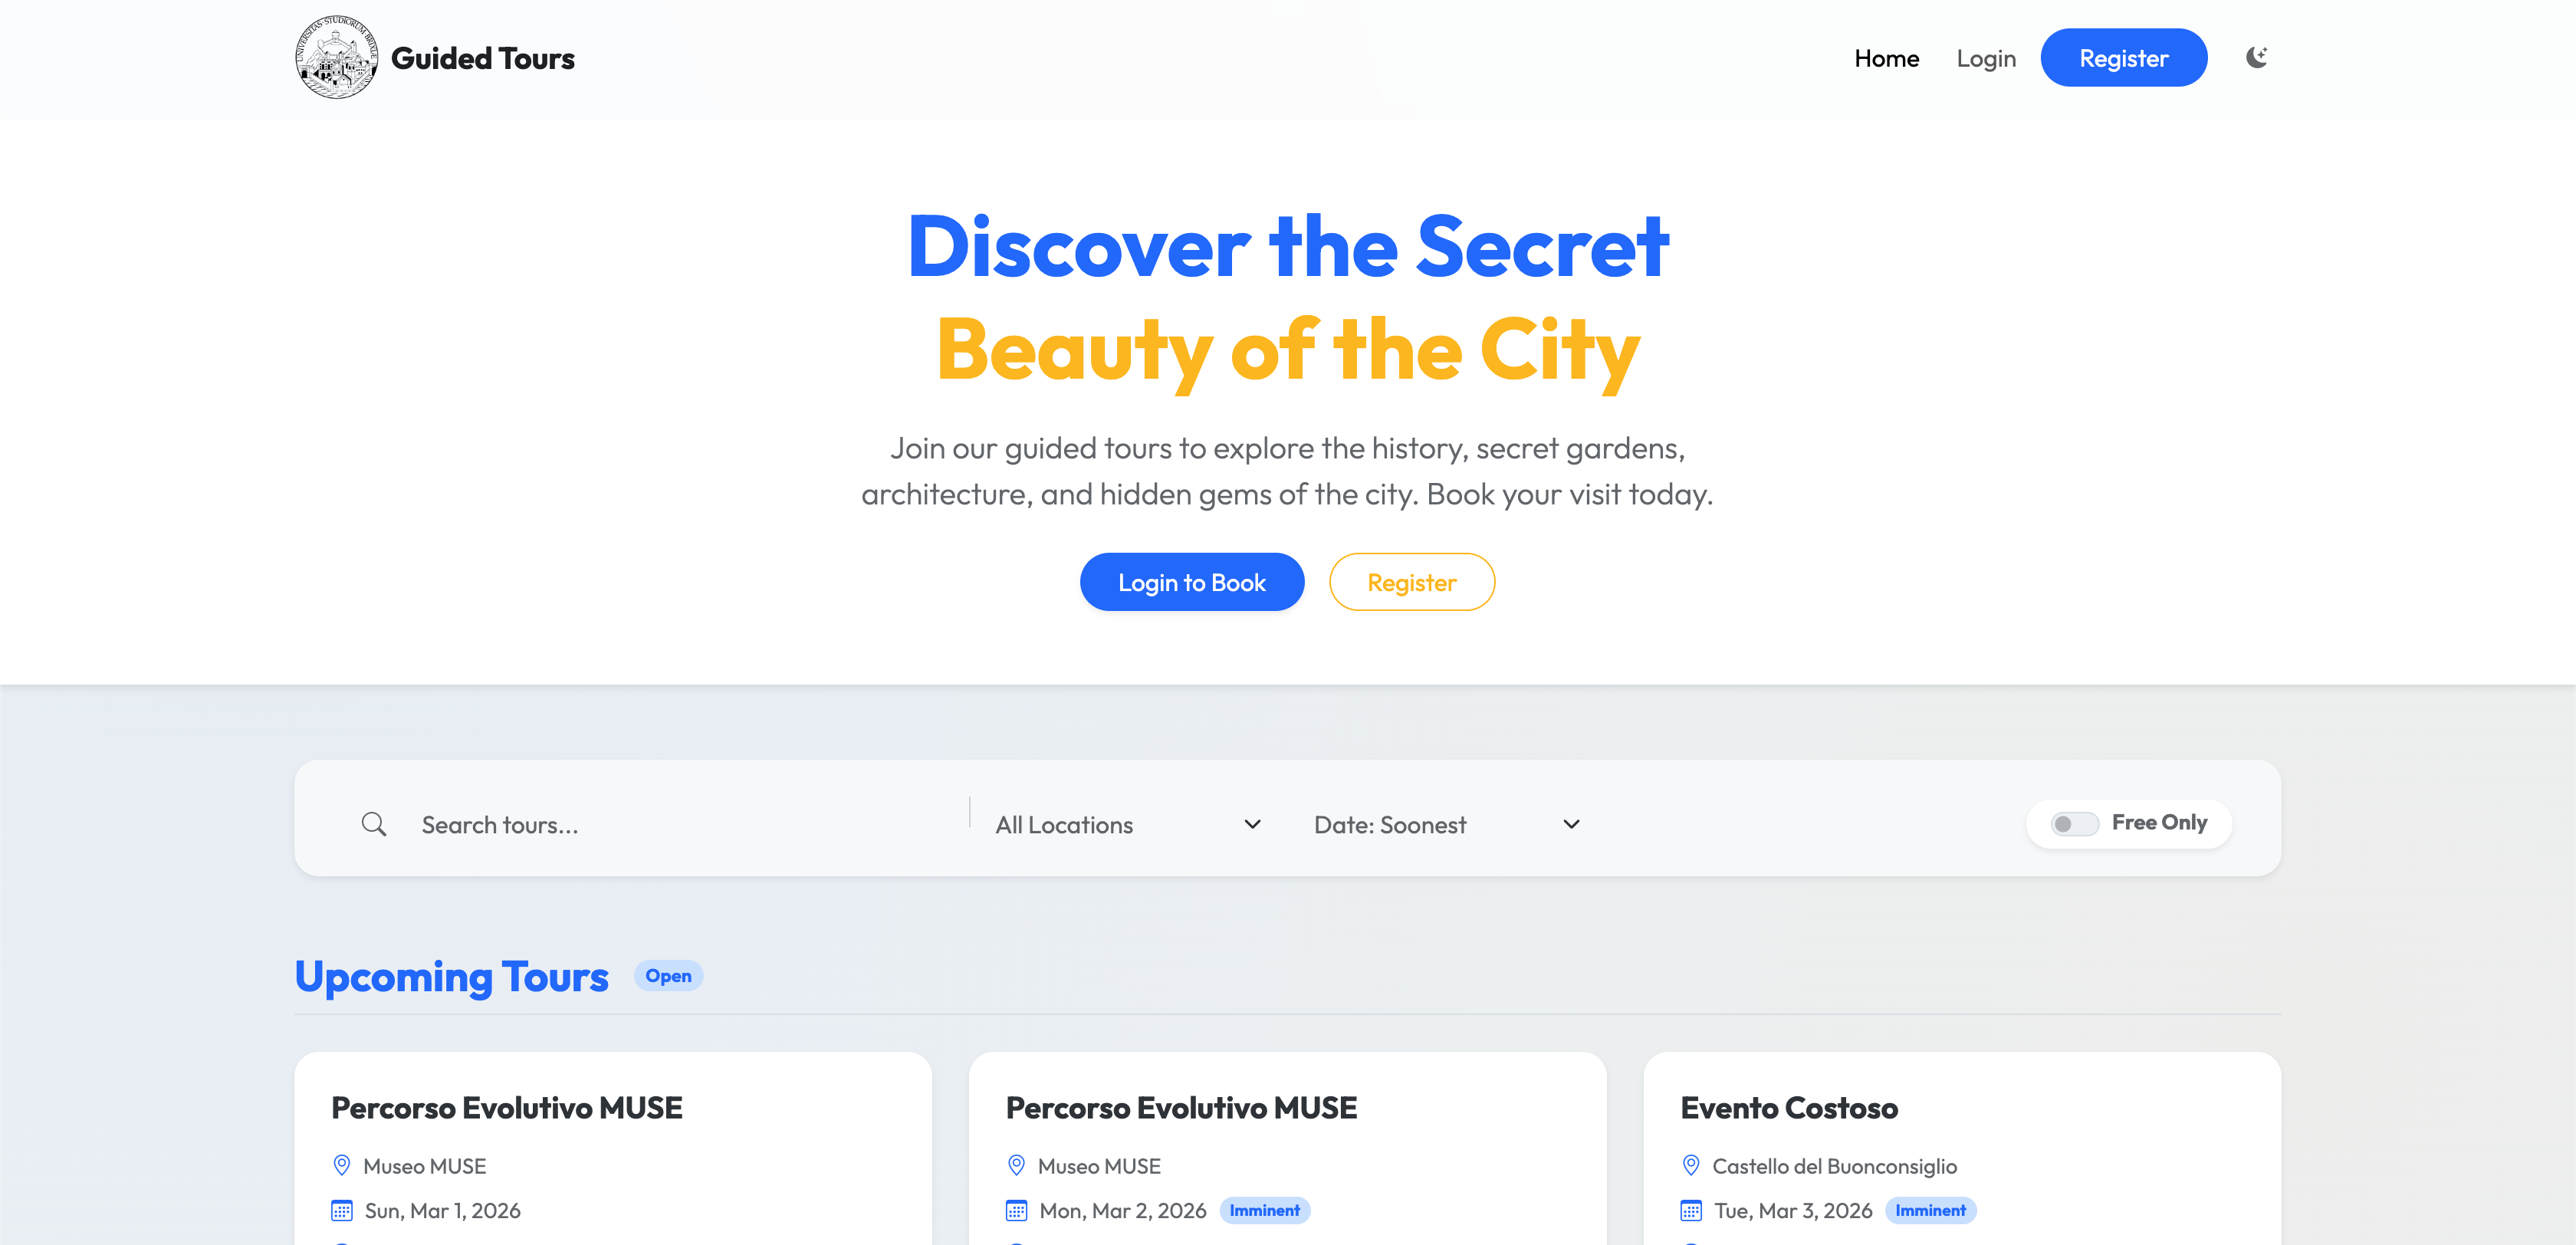
\includegraphics[width=0.9\textwidth, keepaspectratio]{capitoli/immagini/v2/v2_home.png}
    \caption{V2 -- Homepage in modalità ospite (utente non autenticato).}
    \label{fig:v2_home}
\end{figure}

\subsection{Autenticazione}

Le pagine di Login e Register nella V2 sono state semplificate e arricchite di meccanismi di supporto: toggle per la visibilità della password, validazione live dei campi e link diretto al recupero delle credenziali.

\begin{figure}[H]
    \centering
    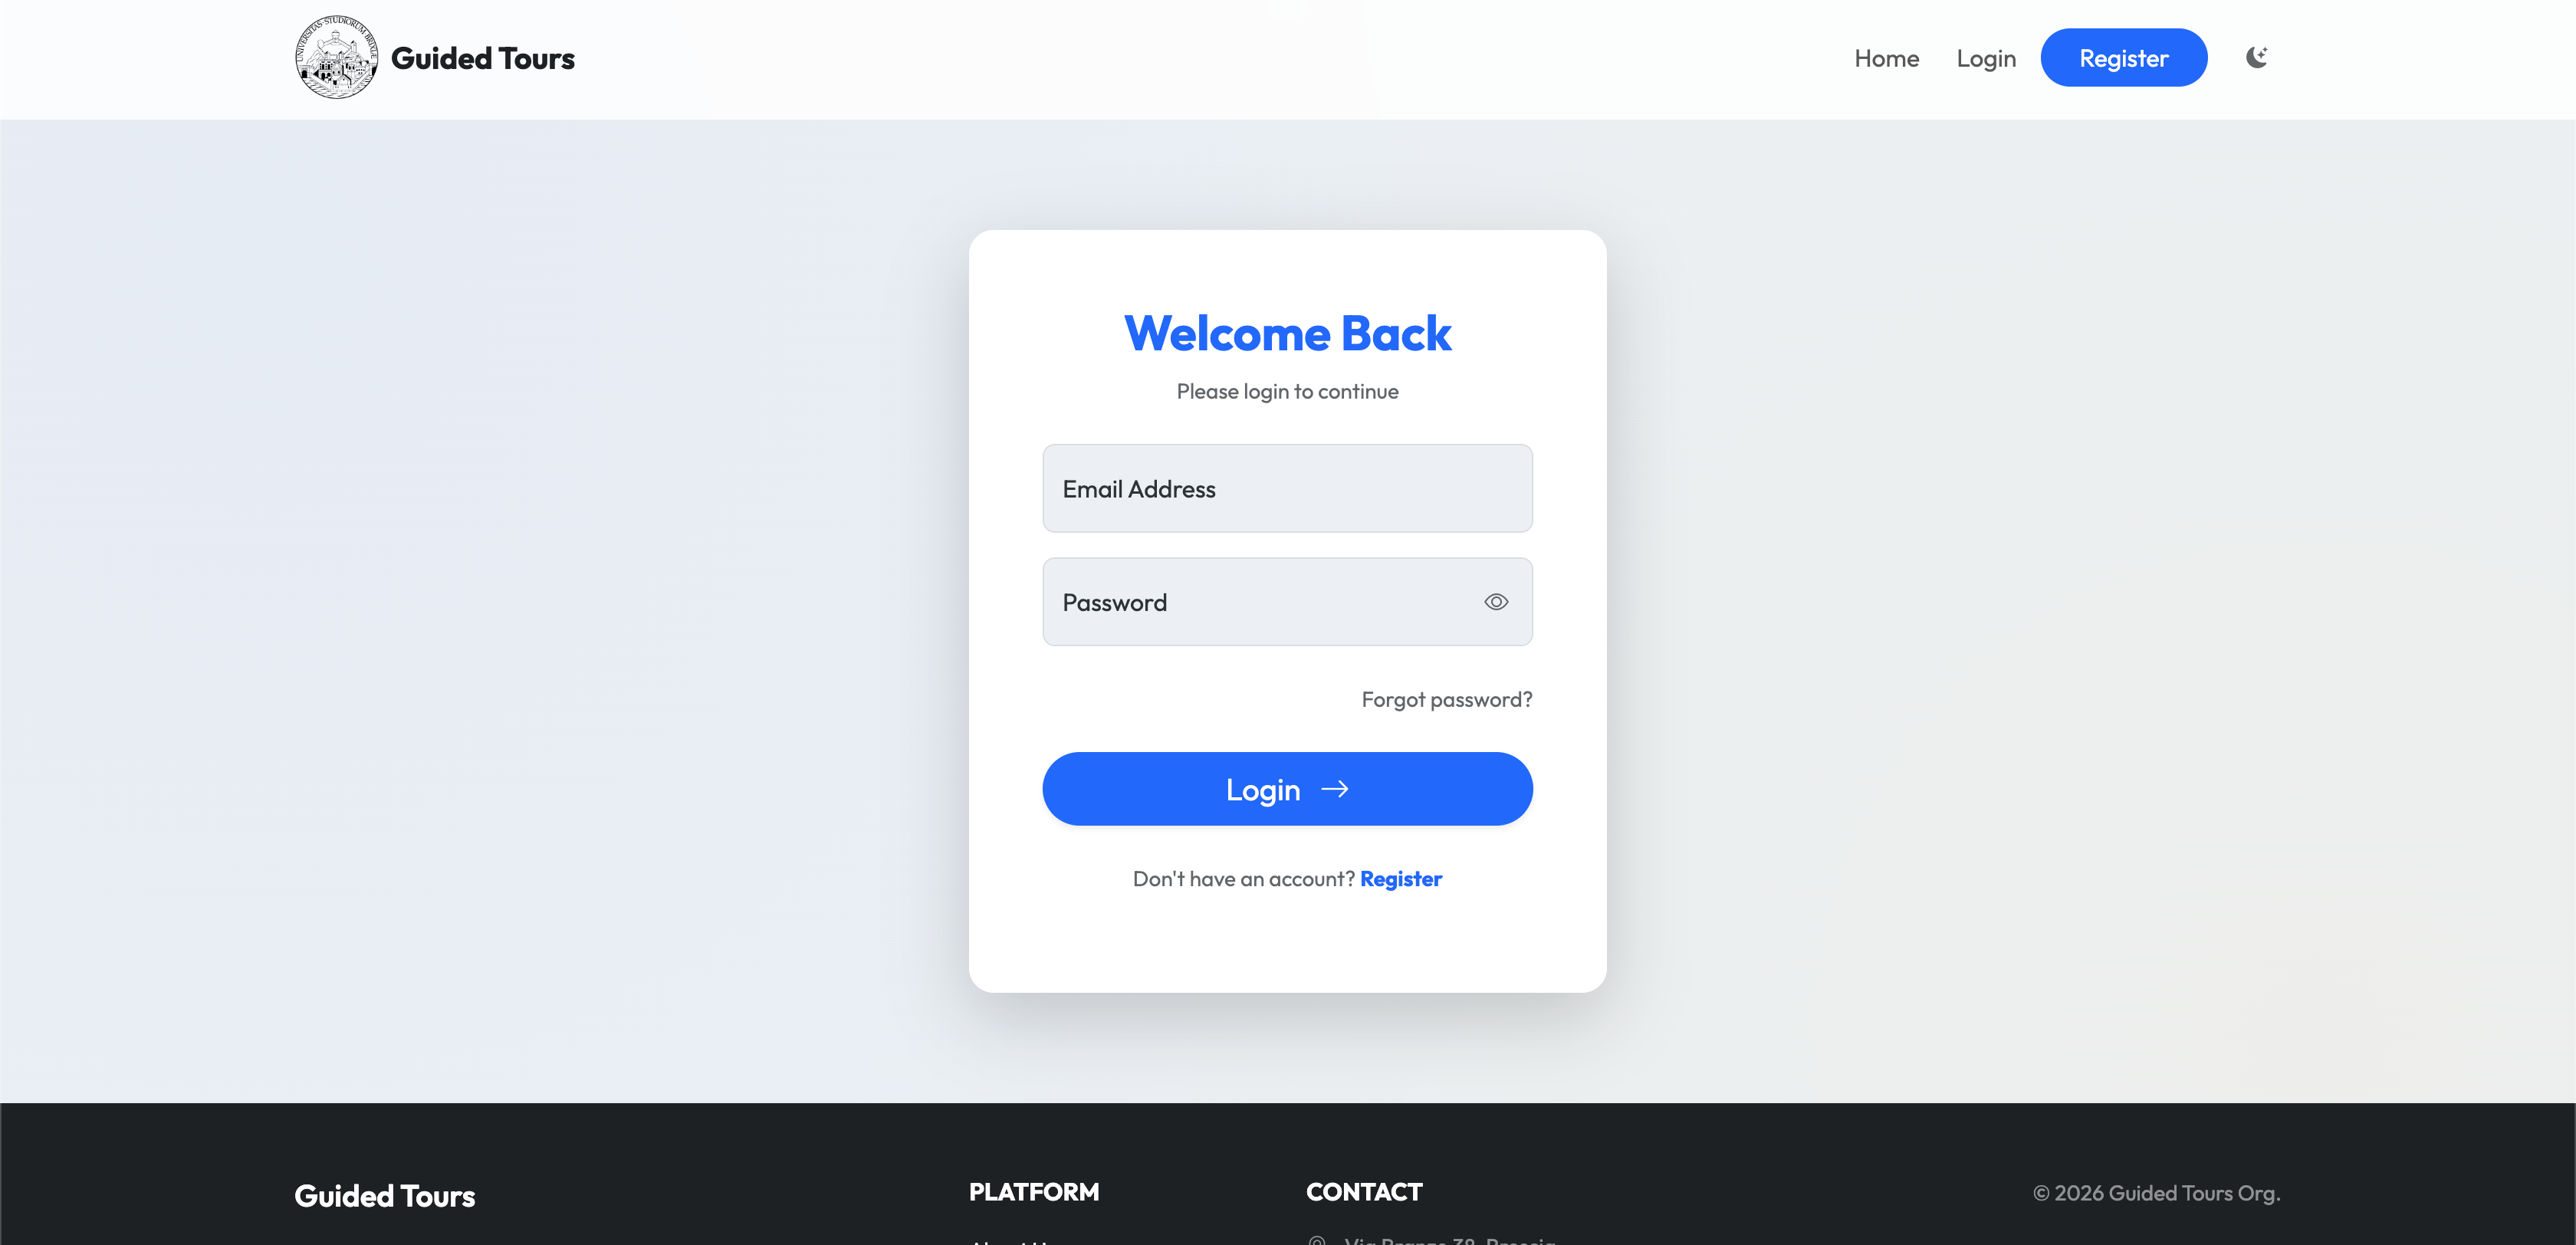
\includegraphics[width=0.9\textwidth, keepaspectratio]{capitoli/immagini/v2/v2_login.png}
    \caption{V2 -- Pagine di Autenticazione (Login e Register).}
    \label{fig:v2_auth}
\end{figure}

\subsection{Dashboard Fruitore}

La Dashboard del Customer nella V2 mostra le prenotazioni attive con il booking code in evidenza, la codifica cromatica semantica degli stati visita e il pulsante di cancellazione con modale di conferma.

\begin{figure}[H]
    \centering
    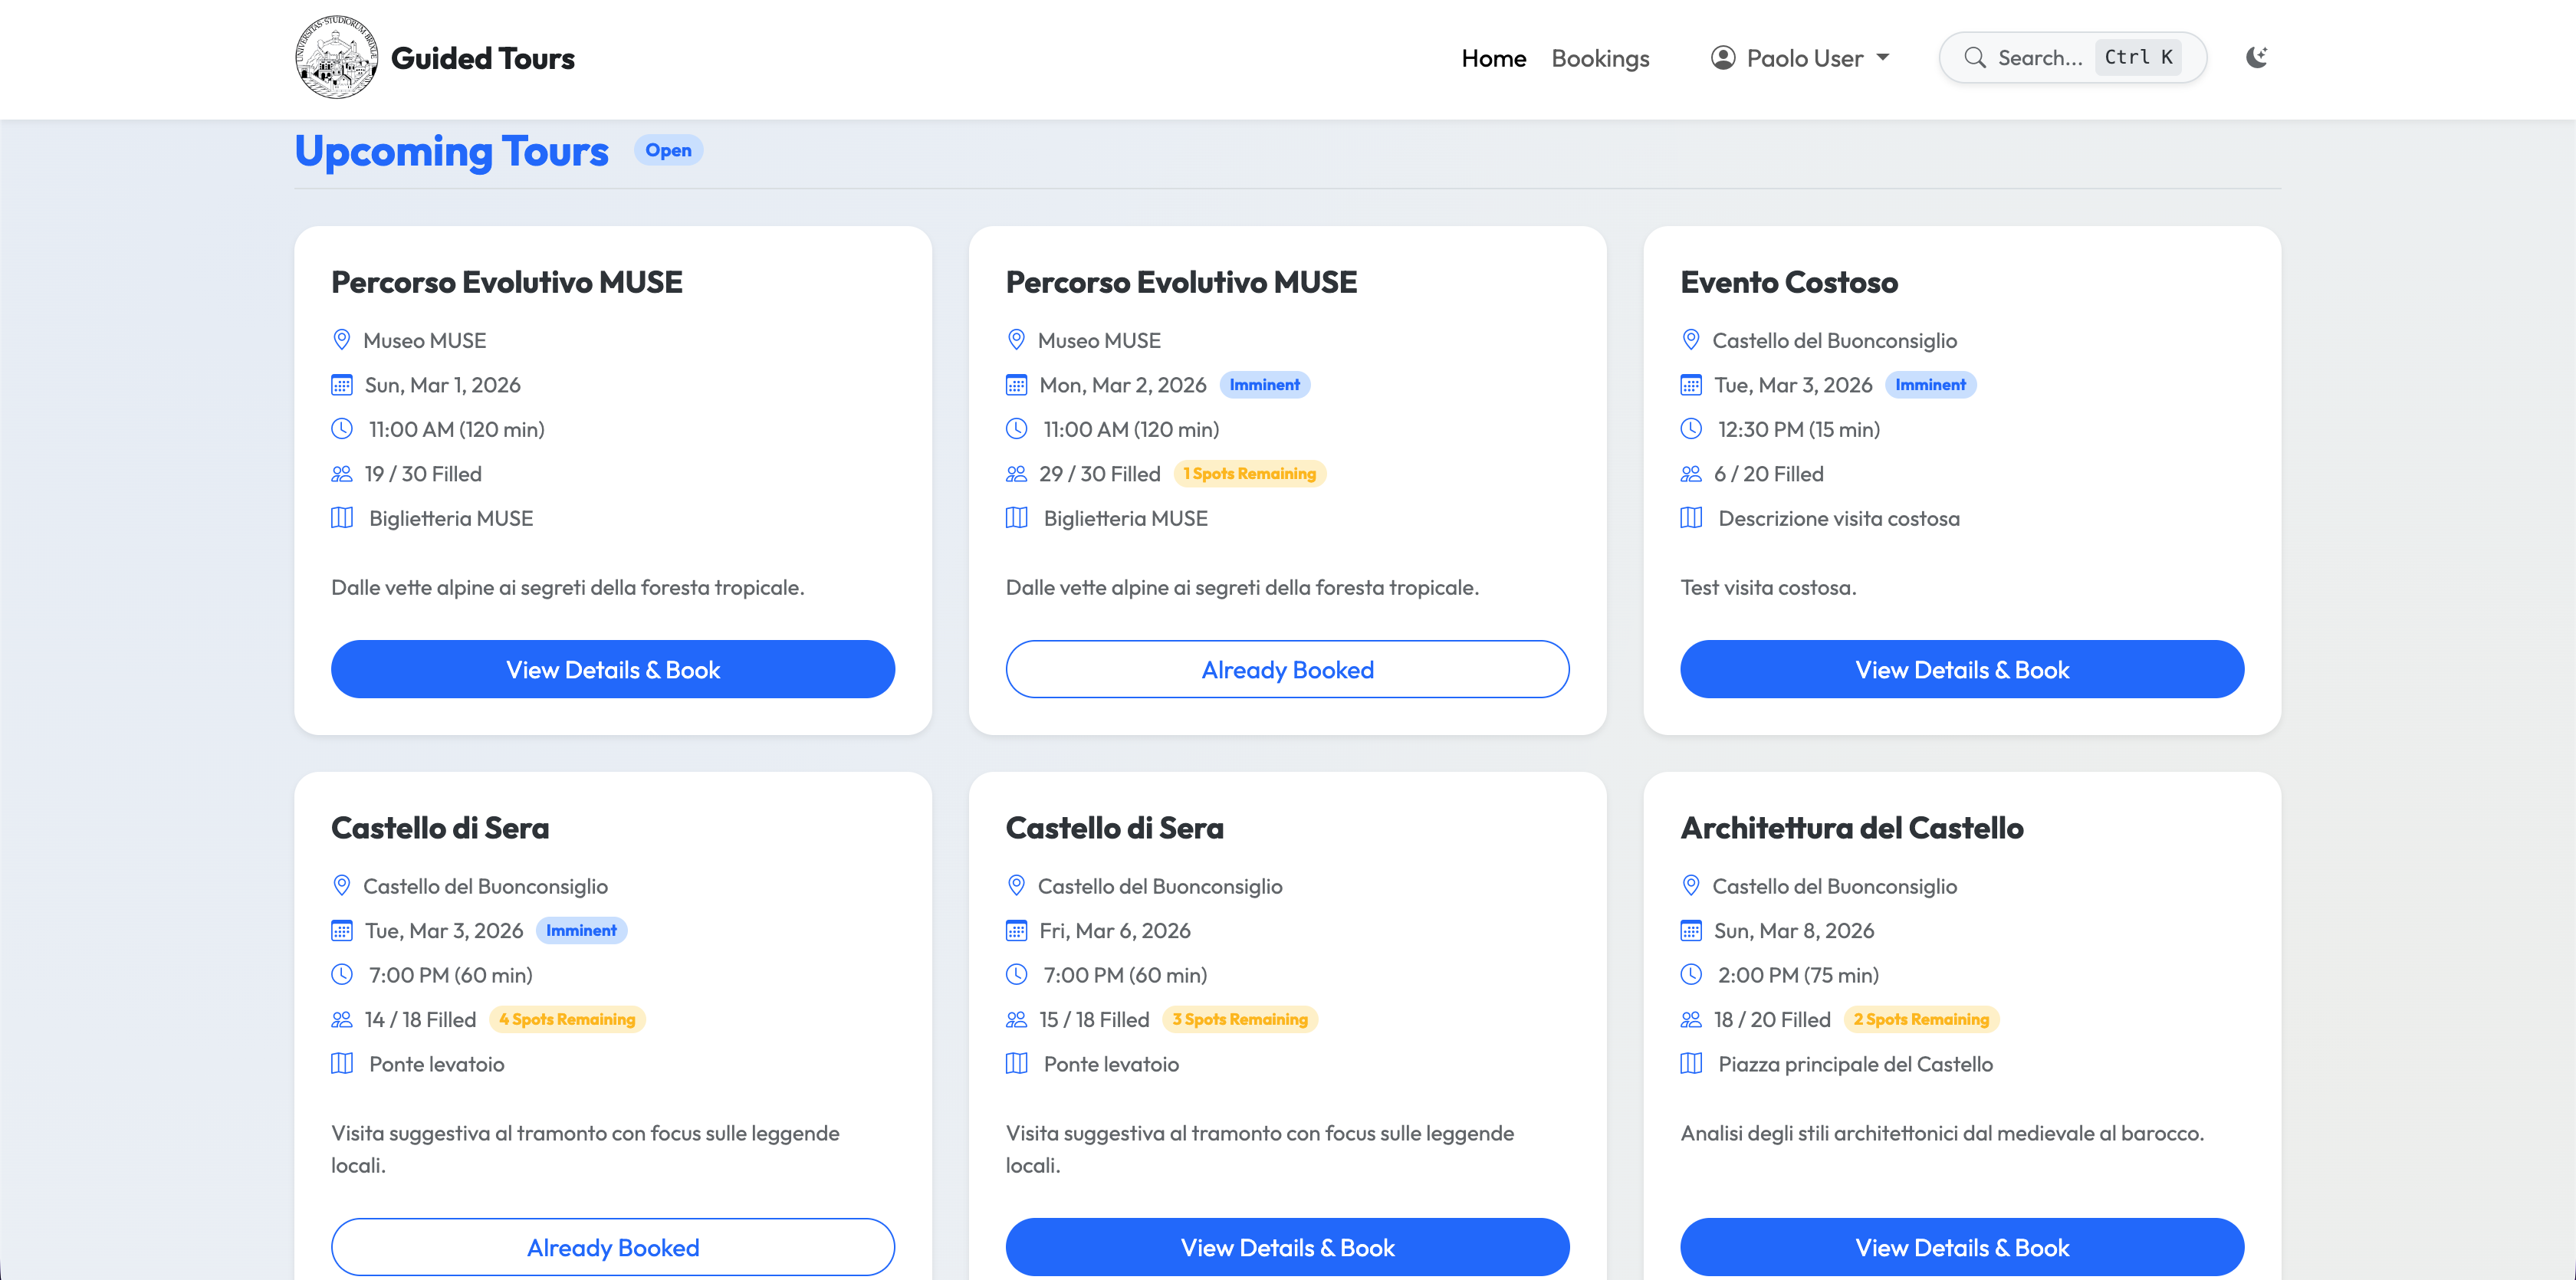
\includegraphics[width=0.9\textwidth, keepaspectratio]{capitoli/immagini/v2/v2_dashboard.png}
    \caption{V2 -- Dashboard Fruitore: prenotazioni attive con booking code, badge di stato e azioni disponibili.}
    \label{fig:v2_dashboard}
\end{figure}

\subsection{Area Amministratore}

Il pannello amministrativo comprende il configuratore a schede (Places, Visit Types, Users), il pannello di Visit Planning con raggruppamento mensile e il form di creazione visite con flusso guidato step-by-step.

\begin{figure}[H]
    \centering
    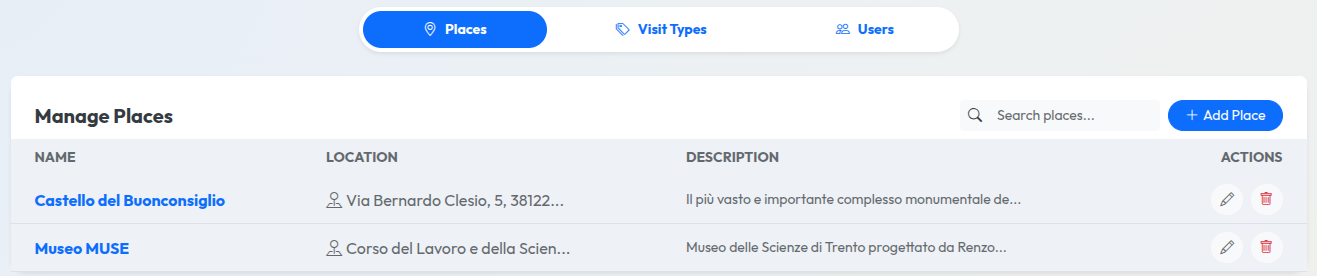
\includegraphics[width=0.9\textwidth, keepaspectratio]{capitoli/immagini/v2/v2_admin_conf.png}
    \caption{V2 -- Admin Configurator: pannello a schede per la gestione centralizzata delle entità del sistema.}
    \label{fig:v2_admin_conf}
\end{figure}

\begin{figure}[H]
    \centering
    \begin{subfigure}[b]{0.47\textwidth}
        \centering
        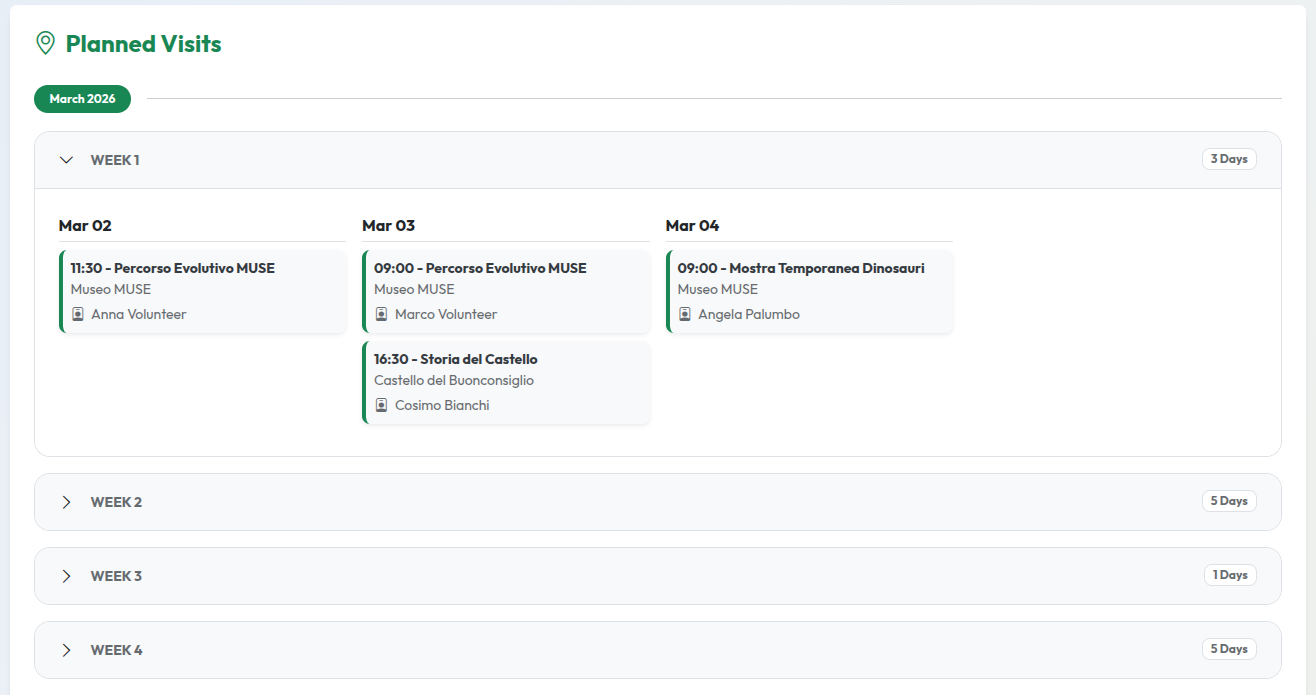
\includegraphics[width=\textwidth, keepaspectratio]{capitoli/immagini/v2/v2_add_visit.png}
        \caption{V1 (Prima)}
    \end{subfigure}
    \hfill
    \begin{subfigure}[b]{0.47\textwidth}
        \centering
        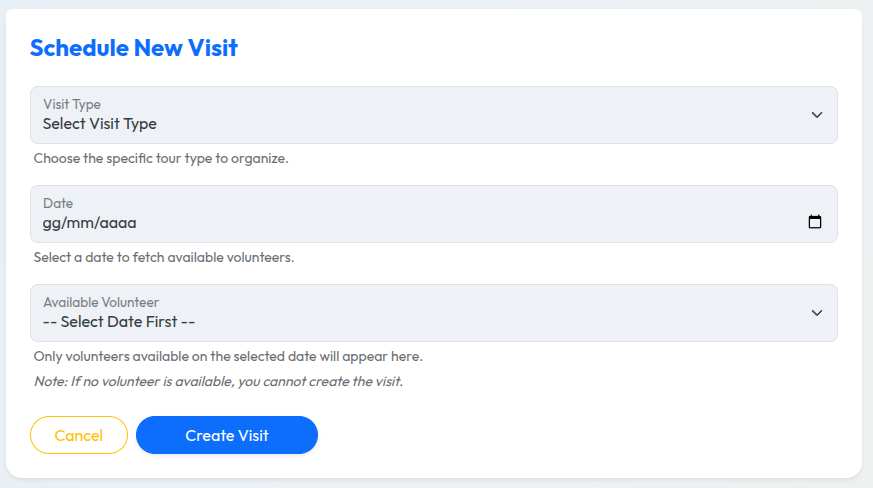
\includegraphics[width=\textwidth, keepaspectratio]{capitoli/immagini/v2/v2_admin_planning.png}
        \caption{V2 (Dopo)}
    \end{subfigure}
    \caption{V2 -- Visit Planning raggruppato per mese (sinistra) e form Add Visit con flusso guidato (destra).}
    \label{fig:v2_planning}
\end{figure}

\subsection{Area Volontario (Guida)}

L'area riservata alle Guide presenta la pagina delle visite assegnate con banner operativo e il calendario per la dichiarazione delle disponibilità mensili.

\begin{figure}[H]
    \centering
    \begin{subfigure}[b]{0.47\textwidth}
        \centering
        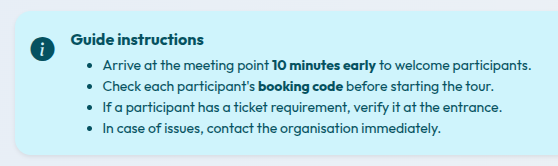
\includegraphics[width=\textwidth, keepaspectratio]{capitoli/immagini/v2/v2_guide_visits.png}
        \caption{V1 (Prima)}
    \end{subfigure}
    \hfill
    \begin{subfigure}[b]{0.47\textwidth}
        \centering
        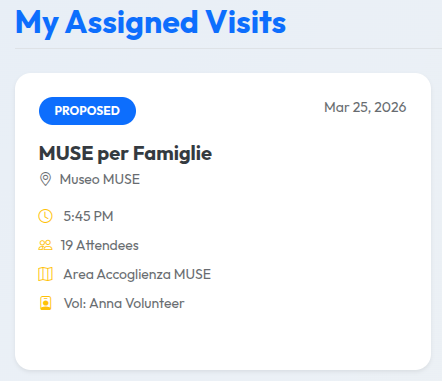
\includegraphics[width=\textwidth, keepaspectratio]{capitoli/immagini/v2/v2_guide_calendar.png}
        \caption{V2 (Dopo)}
    \end{subfigure}
    \caption{V2 -- "My Assigned Visits" con banner istruzioni operative (sinistra) e calendario disponibilità (destra).}
    \label{fig:v2_guide}
\end{figure}

% ─────────────────────────────────────────────────────────────────────────────
\newpage
\section{Riepilogo Interventi per Area}
\label{sec:riepilogo}

I paragrafi precedenti hanno descritto le soluzioni architetturali e i pattern adottati nella riprogettazione. In questa sezione viene fornita una mappatura diretta tra i singoli problemi identificati nel Capitolo 3 e gli interventi implementati, organizzata per area funzionale dell'applicativo.

\subsection{Homepage e Navigazione Globale}

\begin{table}[H]
\centering
\renewcommand{\arraystretch}{1.4}
\small
\begin{tabularx}{\textwidth}{|c|X|c|X|}
\hline
\textbf{P\#} & \textbf{Problema} & \textbf{Sev.} & \textbf{Soluzione adottata} \\ \hline
3  & Semantica colore "Proposed"        & 2 & Stato rinominato "Upcoming"; badge \texttt{bg-primary-subtle} (blu neutrale) in tutte le viste. \\ \hline
4  & Inconsistenza cromatica "Proposed" & 2 & Uso sistematico di \texttt{bg-primary-subtle}: eliminata la variante gialla. \\ \hline
5  & Chiarezza nota pagamento           & 2 & Prezzo esplicito su ogni card (\textit{Free} oppure \textit{€X}); rimosso l'avviso generico ambiguo. \\ \hline
6  & Stile nota pagamento               & 2 & Avviso riformulato come banner \texttt{alert-warning} con icona Bootstrap, ad alto contrasto. \\ \hline
7  & Ambiguità cromatica stati visita   & 1 & "Confirmed" → \texttt{bg-success}; "Complete" → \texttt{bg-secondary}: distinzione cromatica netta. \\ \hline
8  & Mancanza feedback disponibilità    & 1 & Aggiunto badge "Filling Fast" e contatore "X/Y Filled" su ogni card tour. \\ \hline
9  & Ridondanza "Visite confermate"     & 1 & Sezioni "Upcoming" e "Your Confirmed" mantenute distinte con intestazioni esplicite. \\ \hline
10 & Area cliccabile limitata           & 2 & Tutta la card è cliccabile tramite \texttt{stretched-link}; aggiunta classe \texttt{card-hover}. \\ \hline
11 & Gerarchia visiva debole            & 1 & Gerarchia tipografica \texttt{display-4} → \texttt{h3} → \texttt{h5} con Bootstrap; titoli in grassetto. \\ \hline
12 & Assenza shortcut area personale    & 1 & Bottone "My Dashboard" nell'hero section, visibile solo agli utenti autenticati. \\ \hline
—  & Mancanza personalizzazione Homepage & 1 & Sottotitolo hero personalizzato per ruolo: testo specifico per Guest, Customer, Guide e Admin. \\ \hline
\end{tabularx}
\caption{Interventi sulla Homepage e sulla navigazione globale.}
\label{tab:fix_home}
\end{table}

\begin{figure}[H]
    \centering
    \begin{subfigure}[b]{0.47\textwidth}
        \centering
        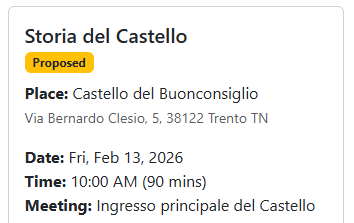
\includegraphics[width=\textwidth, keepaspectratio]{capitoli/immagini/p1.png}
        \caption{V1 (Prima)}
    \end{subfigure}
    \hfill
    \begin{subfigure}[b]{0.47\textwidth}
        \centering
        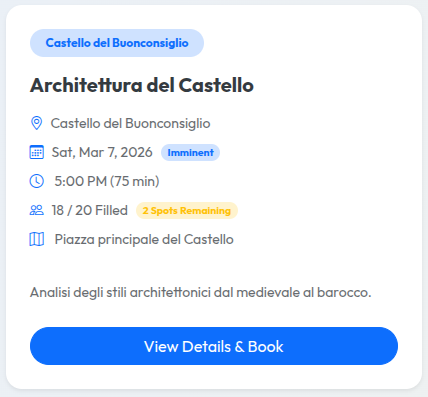
\includegraphics[width=\textwidth, keepaspectratio]{capitoli/immagini/v2/p3_v2.png}
        \caption{V2 (Dopo)}
    \end{subfigure}
    \caption{Fix P.3 -- Semantica colore stato visita: V1 a sinistra (badge giallo "Proposed"), V2 a destra (badge blu neutrale "Upcoming").}
    \label{fig:fix_p3}
\end{figure}

\begin{figure}[H]
    \centering
    \begin{subfigure}[b]{0.47\textwidth}
        \centering
        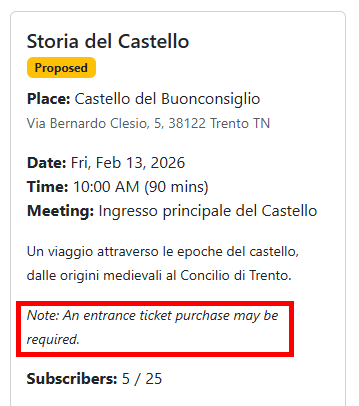
\includegraphics[width=\textwidth, keepaspectratio]{capitoli/immagini/p3.png}
        \caption{V1 (Prima)}
    \end{subfigure}
    \hfill
    \begin{subfigure}[b]{0.47\textwidth}
        \centering
        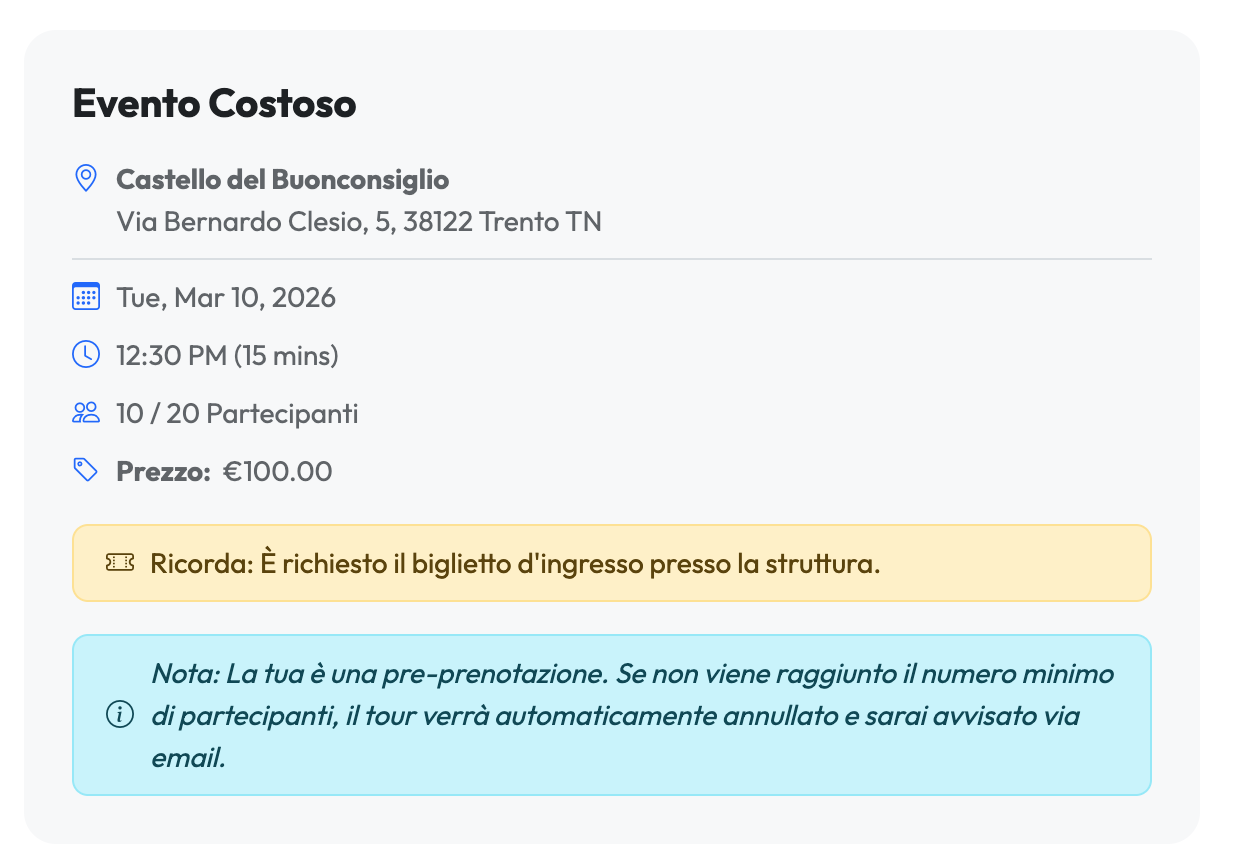
\includegraphics[width=\textwidth, keepaspectratio]{capitoli/immagini/v2/p6_v2.png}
        \caption{V2 (Dopo)}
    \end{subfigure}
    \caption{Fix P.6 -- Nota pagamento: V1 a sinistra (testo generico poco visibile), V2 a destra (banner \texttt{alert-warning} con icona).}
    \label{fig:fix_p6}
\end{figure}

\subsection{Footer e Navbar}

\begin{table}[H]
\centering
\renewcommand{\arraystretch}{1.4}
\small
\begin{tabularx}{\textwidth}{|c|X|c|X|}
\hline
\textbf{P\#} & \textbf{Problema} & \textbf{Sev.} & \textbf{Soluzione adottata} \\ \hline
13 & Incoerenza linguistica  & 1 & Footer interamente riscritto in inglese; rimossa la dicitura italiana "Sito di visite guidate". \\ \hline
35 & Email non cliccabili    & 2 & Tutti gli indirizzi email nel footer avvolti da tag \texttt{<a href="mailto:...">}. \\ \hline
\end{tabularx}
\caption{Interventi su Footer e Navbar.}
\label{tab:fix_footer}
\end{table}

\subsection{Autenticazione (Login e Register)}

\begin{table}[H]
\centering
\renewcommand{\arraystretch}{1.4}
\small
\begin{tabularx}{\textwidth}{|c|X|c|X|}
\hline
\textbf{P\#} & \textbf{Problema} & \textbf{Sev.} & \textbf{Soluzione adottata} \\ \hline
15 & Mancanza toggle visibilità password  & 1 & Icona occhio (Bootstrap Icons) con script JS \texttt{showPassword()} nelle pagine Login e Register. \\ \hline
16 & Navigazione ambigua verso Register   & 1 & Rimossi accessi multipli; unico link "Create an Account" nel footer della card di login. \\ \hline
17 & Ridondanza informativa Ruoli (Login) & 1 & Testo ridondante rimosso; sostituito con l'essenziale "Please login to continue". \\ \hline
18 & Feedback errore non user-friendly    & 1 & Messaggi di errore riformulati e presentati tramite Toast Notifications, chiari e non tecnici. \\ \hline
19 & Assenza recupero password            & 3 & Implementata pagina "Forgot Password" con reset tramite link inviato via email (\texttt{PasswordResetController}). \\ \hline
20 & Carico cognitivo posti disponibili   & 2 & Label esplicita "(X spots remaining)" accanto al campo numero partecipanti nel form di prenotazione. \\ \hline
21 & Navigazione ridondante verso Login   & 1 & Unico link "Already have an account? Login" nella pagina di registrazione. \\ \hline
22 & Ridondanza informativa Ruoli (Register) & 1 & Rimossa spiegazione dei ruoli; form di registrazione semplificato. \\ \hline
23 & Validazione tardiva input            & 2 & Aggiunta validazione JavaScript live: controllo lunghezza e corrispondenza password in tempo reale. \\ \hline
\end{tabularx}
\caption{Interventi sull'autenticazione.}
\label{tab:fix_auth}
\end{table}

\begin{figure}[H]
    \centering
    \begin{subfigure}[b]{0.47\textwidth}
        \centering
        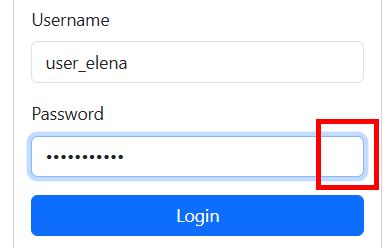
\includegraphics[width=\textwidth, keepaspectratio]{capitoli/immagini/p11.png}
        \caption{V1 (Prima)}
    \end{subfigure}
    \hfill
    \begin{subfigure}[b]{0.47\textwidth}
        \centering
        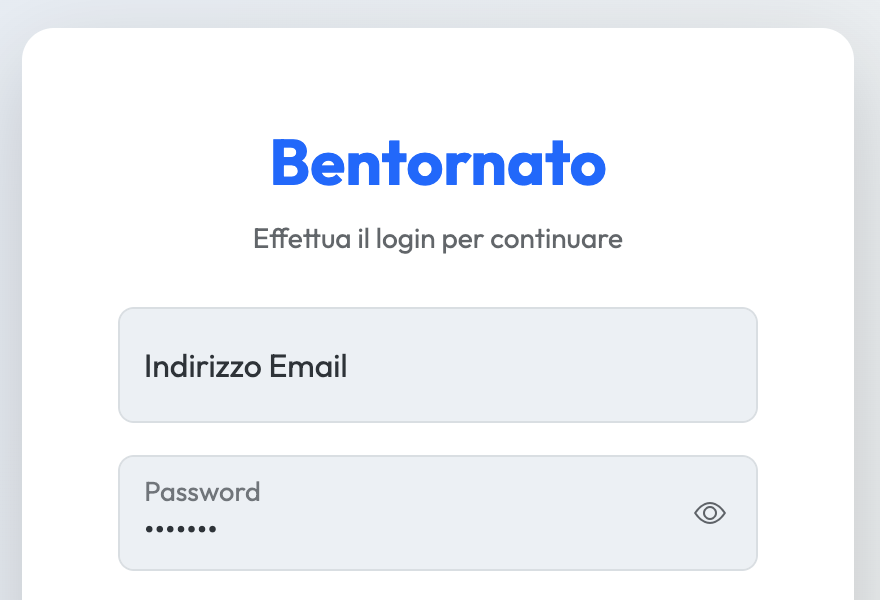
\includegraphics[width=\textwidth, keepaspectratio]{capitoli/immagini/v2/p15_v2.png}
        \caption{V2 (Dopo)}
    \end{subfigure}
    \caption{Fix P.15 -- Toggle visibilità password: V1 a sinistra (campo senza icona), V2 a destra (icona occhio per mostrare/nascondere la password).}
    \label{fig:fix_p15}
\end{figure}

\begin{figure}[H]
    \centering
    \begin{subfigure}[b]{0.47\textwidth}
        \centering
        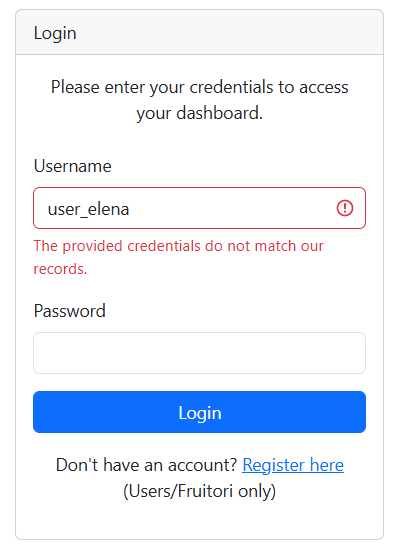
\includegraphics[width=\textwidth, keepaspectratio]{capitoli/immagini/p17.png}
        \caption{V1 (Prima)}
    \end{subfigure}
    \hfill
    \begin{subfigure}[b]{0.47\textwidth}
        \centering
        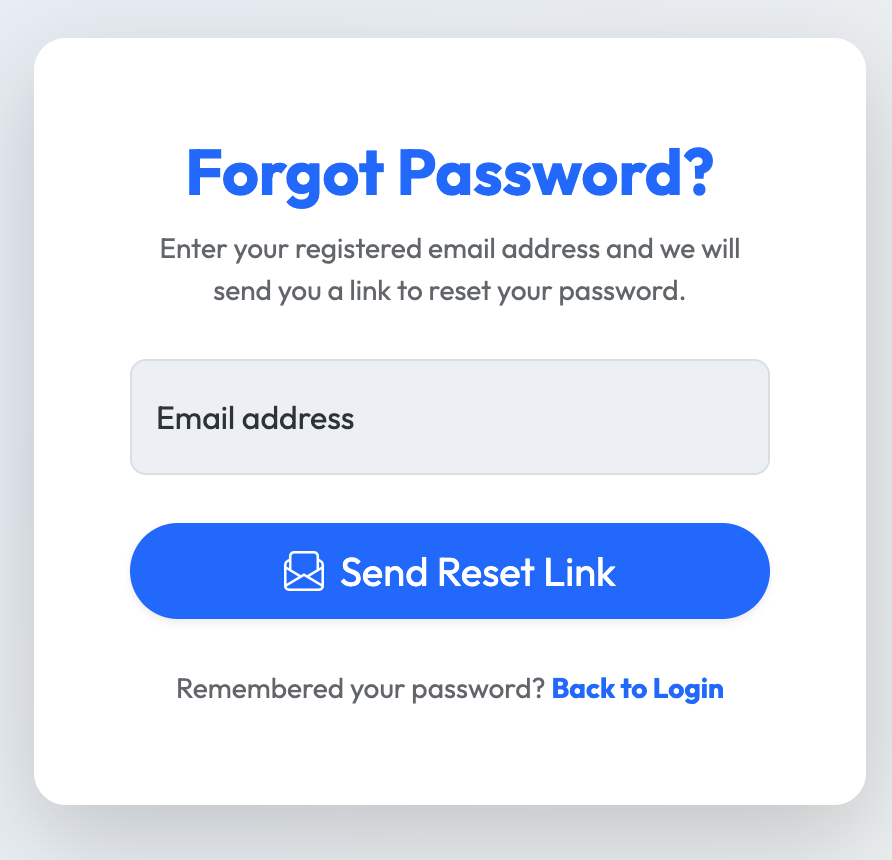
\includegraphics[width=\textwidth, keepaspectratio]{capitoli/immagini/v2/p19_v2.png}
        \caption{V2 (Dopo)}
    \end{subfigure}
    \caption{Fix P.19 -- Recupero password: V1 a sinistra (nessun link di recupero), V2 a destra (pagina "Forgot Password" dedicata).}
    \label{fig:fix_p19}
\end{figure}

\begin{figure}[H]
    \centering
    \begin{subfigure}[b]{0.47\textwidth}
        \centering
        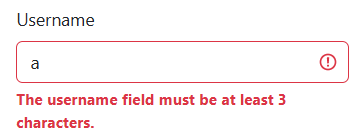
\includegraphics[width=\textwidth, keepaspectratio]{capitoli/immagini/p21.png}
        \caption{V1 (Prima)}
    \end{subfigure}
    \hfill
    \begin{subfigure}[b]{0.47\textwidth}
        \centering
        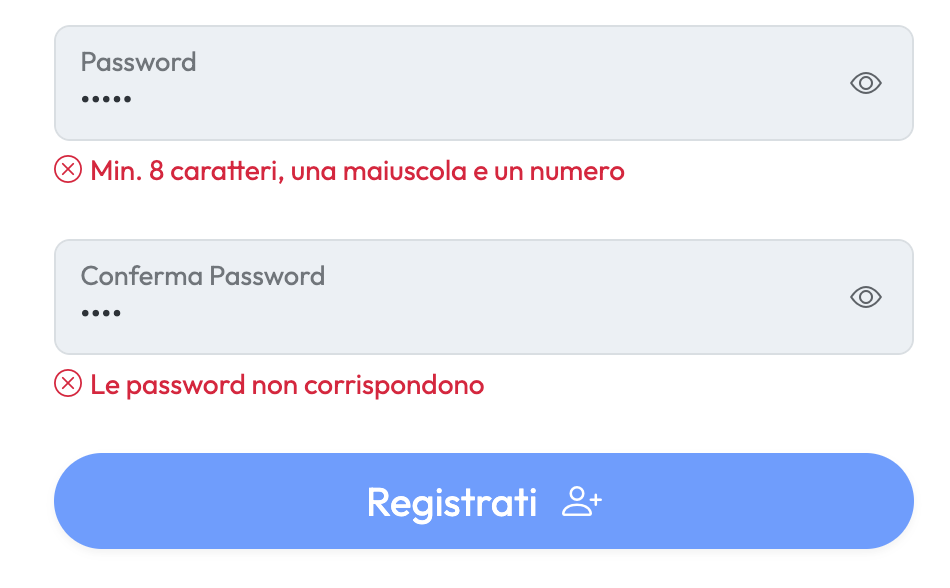
\includegraphics[width=\textwidth, keepaspectratio]{capitoli/immagini/v2/p23_v2.png}
        \caption{V2 (Dopo)}
    \end{subfigure}
    \caption{Fix P.23 -- Validazione live password: V1 a sinistra (nessun feedback), V2 a destra (indicatori in tempo reale su lunghezza e corrispondenza).}
    \label{fig:fix_p23}
\end{figure}

\subsection{Dashboard Fruitore}

\begin{table}[H]
\centering
\renewcommand{\arraystretch}{1.4}
\small
\begin{tabularx}{\textwidth}{|c|X|c|X|}
\hline
\textbf{P\#} & \textbf{Problema} & \textbf{Sev.} & \textbf{Soluzione adottata} \\ \hline
24 & Visibilità "Booking code"            & 1 & Codice visualizzato in font monospaziato bold con etichetta "Booking Code" esplicita. \\ \hline
25 & Ambiguità etichetta "Participant"    & 2 & Etichetta standardizzata "X Participants" coerente con il resto dell'interfaccia. \\ \hline
26 & Affordance ingannevole "My Booking" & 2 & Rimosso il menu a tendina ambiguo; sostituito con bottone esplicito \texttt{btn-danger} "Cancel Booking". \\ \hline
27 & Stile pulsante eliminazione          & 1 & Pulsante in stile \texttt{btn-danger} e testo rosso, coerente con il Design System. \\ \hline
\end{tabularx}
\caption{Interventi sulla Dashboard Fruitore.}
\label{tab:fix_dashboard}
\end{table}

\begin{figure}[H]
    \centering
    \begin{subfigure}[b]{0.47\textwidth}
        \centering
        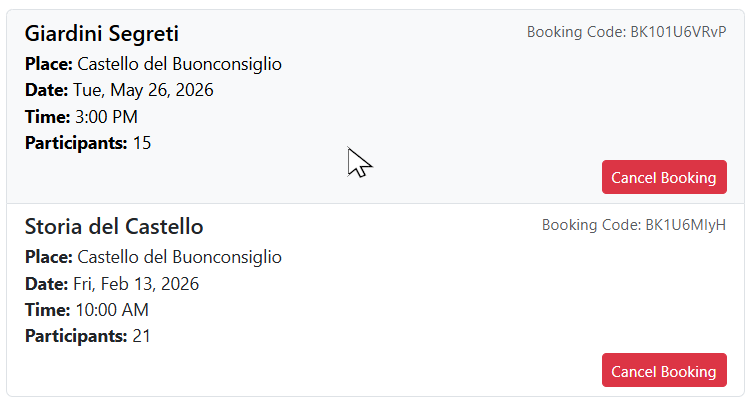
\includegraphics[width=\textwidth, keepaspectratio]{capitoli/immagini/p24.png}
        \caption{V1 (Prima)}
    \end{subfigure}
    \hfill
    \begin{subfigure}[b]{0.40\textwidth}
        \centering
        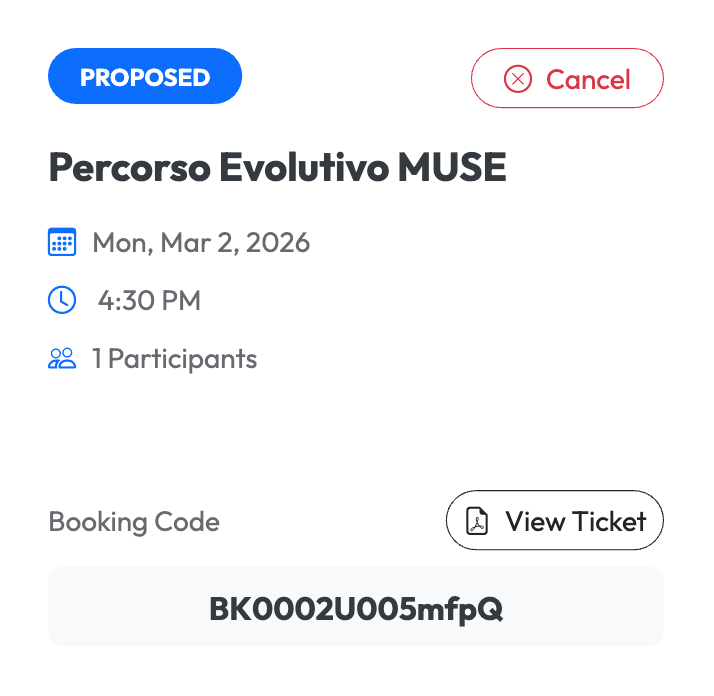
\includegraphics[width=\textwidth, keepaspectratio]{capitoli/immagini/v2/p26_v2.png}
        \caption{V2 (Dopo)}
    \end{subfigure}
    \caption{Fix P.26 -- Affordance "My Booking": V1 a sinistra, V2 a destra (bottone meno impattante "Cancel Booking" con modale di conferma).}
    \label{fig:fix_p26}
\end{figure}

\subsection{Area Amministratore}

\begin{table}[H]
\centering
\renewcommand{\arraystretch}{1.4}
\small
\begin{tabularx}{\textwidth}{|c|X|c|X|}
\hline
\textbf{P\#} & \textbf{Problema} & \textbf{Sev.} & \textbf{Soluzione adottata} \\ \hline
28 & Inconsistenza terminologica            & 1 & "Tours" e "Bookings" lato utente; "Visits" riservato al contesto amministrativo (dominio tecnico corretto). \\ \hline
29 & Incoerenza spaziatura Header           & 1 & Navbar Bootstrap standard con padding uniformi in tutte le pagine. \\ \hline
30 & Validazione tardiva aggiunta utente    & 2 & Validazione JS real-time per la password nel modale di creazione utente (\texttt{admin/configurator}). \\ \hline
31 & Assenza conferma eliminazione          & 4 & Global Delete Confirmation Modal: pop-up obbligatorio con avviso "This action cannot be undone" prima di ogni eliminazione. \\ \hline
32 & Disorganizzazione layout Visit Planning & 1 & Layout a card raggruppate per mese nel pannello \texttt{visit-planning.blade.php}. \\ \hline
33 & Flusso inserimento non intuitivo       & 3 & Flusso guidato in sequenza: selezione Tipo Visita → Data → Volontario disponibile (\texttt{admin/visits/create}). \\ \hline
34 & Mancanza feedback su vincoli           & 3 & Help text espliciti accanto ad ogni campo critico (data minima, assenza volontari disponibili). \\ \hline
40 & Colore bottone non coerente            & 2 & Bottone "Change Password" nel profilo allineato al Design System: rimosso lo stile rosso fuorviante. \\ \hline
\end{tabularx}
\caption{Interventi sull'Area Amministratore.}
\label{tab:fix_admin}
\end{table}

\begin{figure}[H]
    \centering
    \begin{subfigure}[b]{0.47\textwidth}
        \centering
        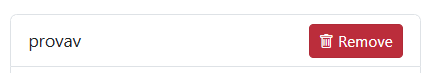
\includegraphics[width=\textwidth, keepaspectratio]{capitoli/immagini/p29.png}
        \caption{V1 (Prima)}
    \end{subfigure}
    \hfill
    \begin{subfigure}[b]{0.47\textwidth}
        \centering
        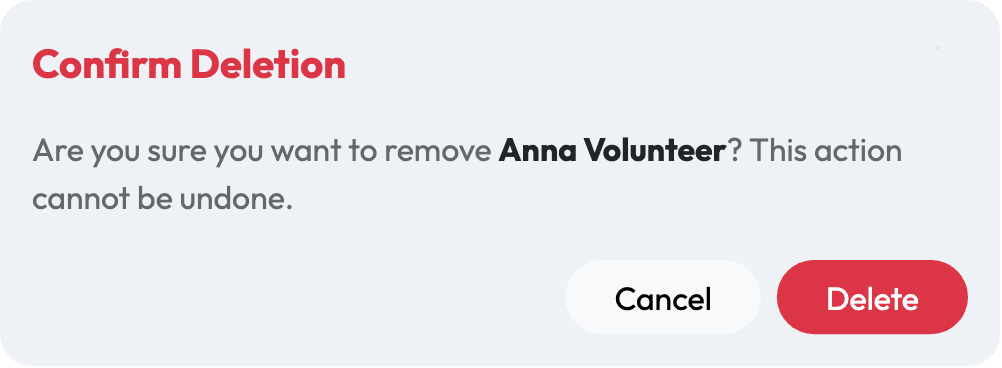
\includegraphics[width=\textwidth, keepaspectratio]{capitoli/immagini/v2/p31_v2.png}
        \caption{V2 (Dopo)}
    \end{subfigure}
    \caption{Fix P.31 -- Conferma eliminazione: V1 a sinistra (eliminazione immediata senza dialogo), V2 a destra (Global Delete Confirmation Modal con avviso "This action cannot be undone").}
    \label{fig:fix_p31}
\end{figure}

\begin{figure}[H]
    \centering
    \begin{subfigure}[b]{0.47\textwidth}
        \centering
        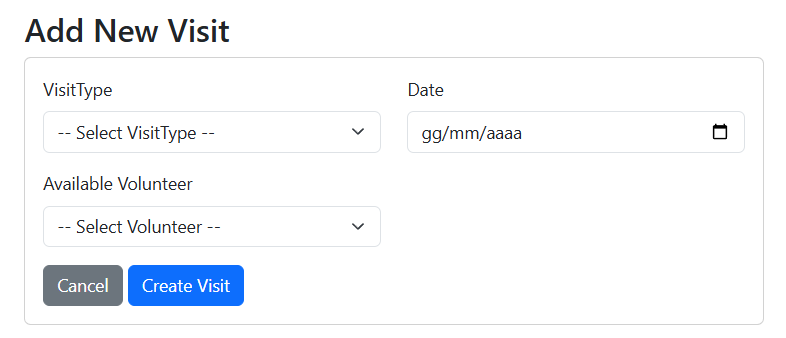
\includegraphics[width=\textwidth, keepaspectratio]{capitoli/immagini/p31.png}
        \caption{V1 (Prima)}
    \end{subfigure}
    \hfill
    \begin{subfigure}[b]{0.47\textwidth}
        \centering
        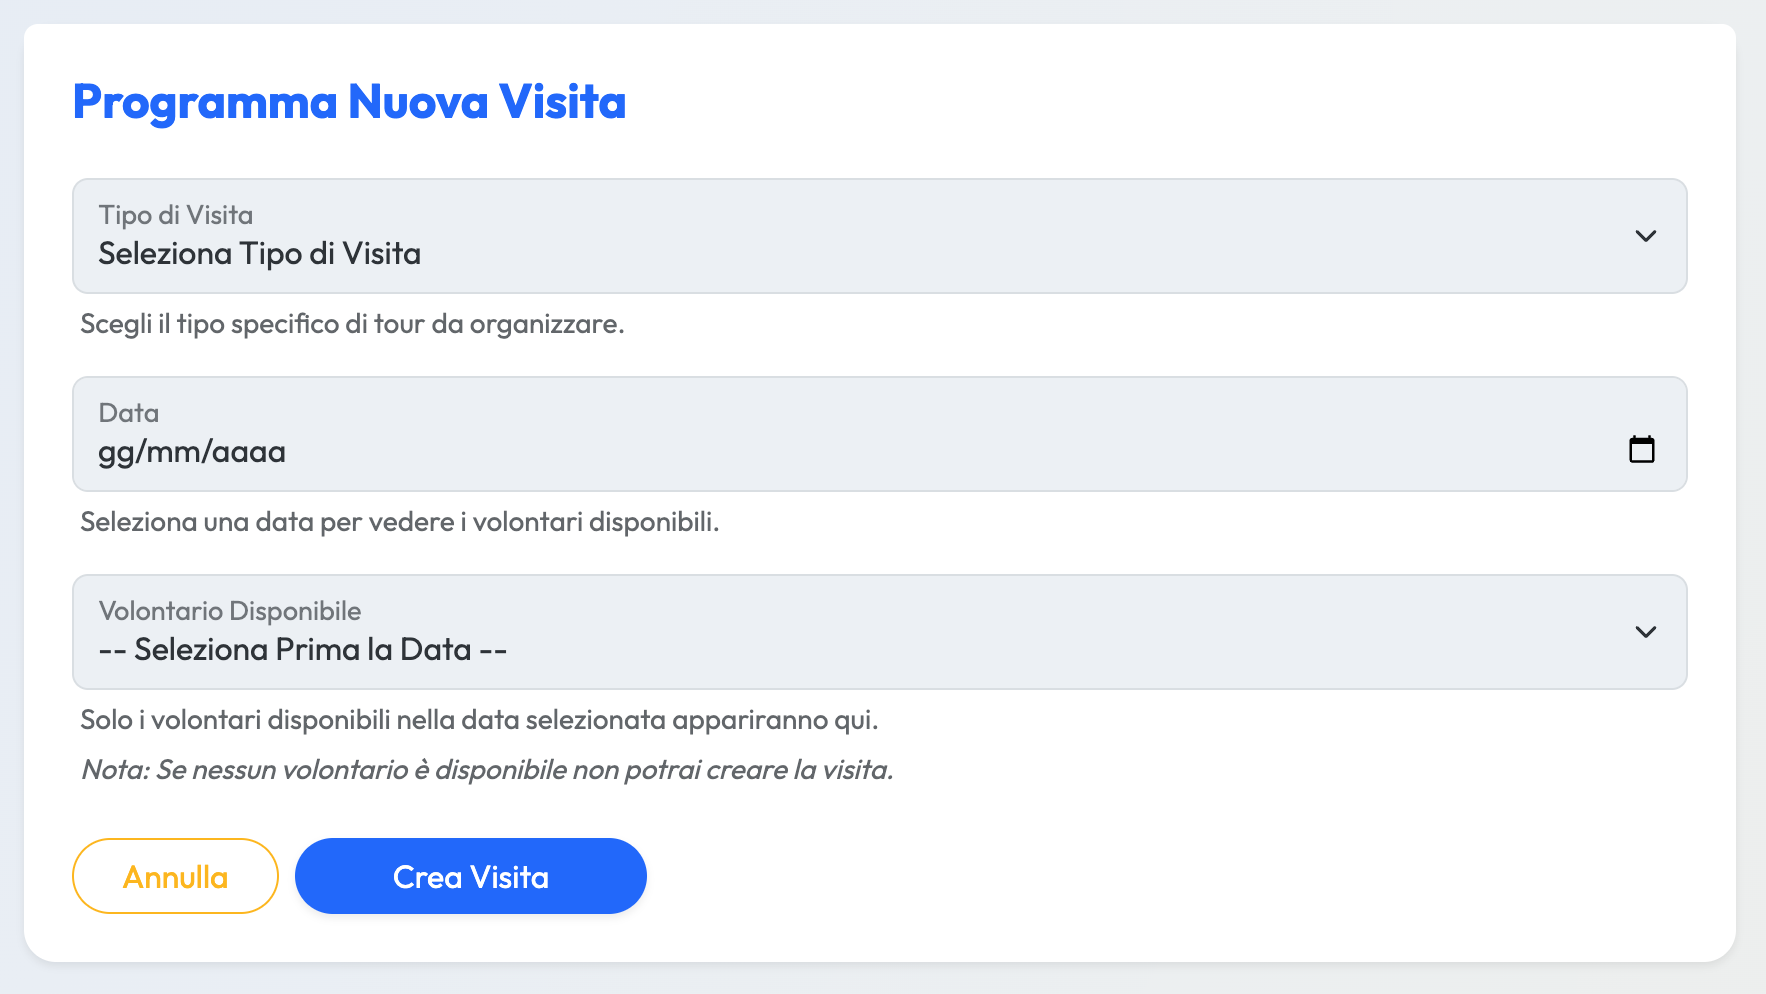
\includegraphics[width=\textwidth, keepaspectratio]{capitoli/immagini/v2/p33_v2.png}
        \caption{V2 (Dopo)}
    \end{subfigure}
    \caption{Fix P.33 -- Flusso inserimento visita: V1 a sinistra (form non guidato), V2 a destra (flusso step-by-step Tipo → Data → Volontario disponibile).}
    \label{fig:fix_p33}
\end{figure}

\subsection{Area Volontario (Guida)}

\begin{table}[H]
\centering
\renewcommand{\arraystretch}{1.4}
\small
\begin{tabularx}{\textwidth}{|c|X|c|X|}
\hline
\textbf{P\#} & \textbf{Problema} & \textbf{Sev.} & \textbf{Soluzione adottata} \\ \hline
37 & Assenza indicazioni operative           & 2 & Banner \texttt{alert-info} con istruzioni operative (puntualità, verifica booking code, gestione imprevisti) nella pagina "My Assigned Visits". \\ \hline
38 & Ridondanza nome volontario nelle card   & 1 & Il nome del volontario assegnato viene nascosto se corrisponde all'utente loggato; visibile solo agli altri ruoli. \\ \hline
\end{tabularx}
\caption{Interventi sull'Area Volontario.}
\label{tab:fix_volontario}
\end{table}

\begin{figure}[H]
    \centering
    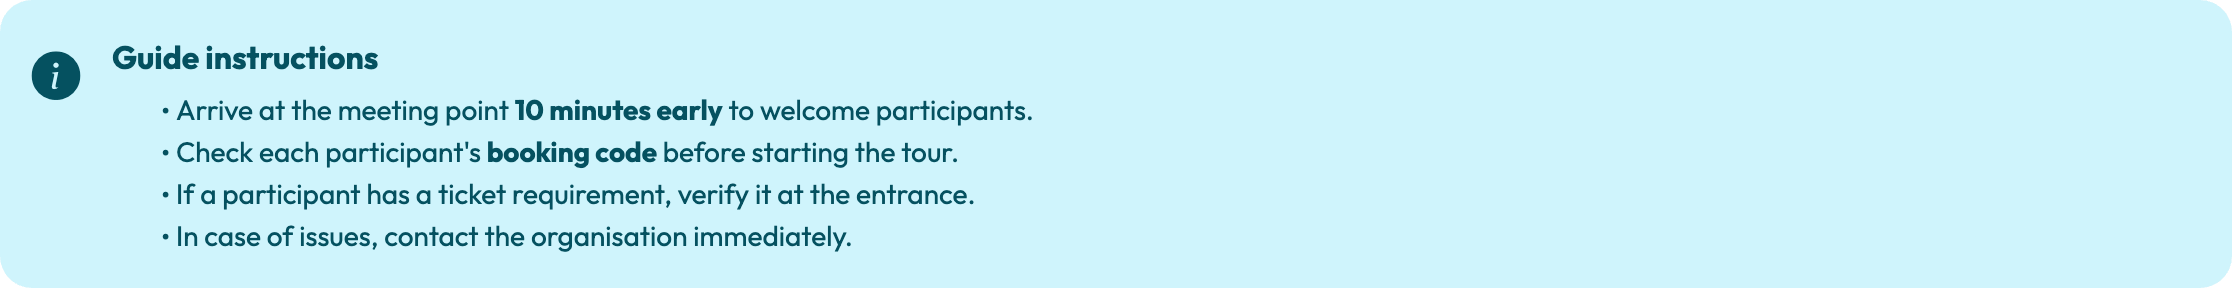
\includegraphics[width=0.85\textwidth, keepaspectratio]{capitoli/immagini/v2/p37_v2.png}
    \caption{Fix P.37 -- Banner istruzioni operative nella pagina "My Assigned Visits": avviso contestuale con promemoria su puntualità, verifica booking code e gestione imprevisti.}
    \label{fig:fix_p37}
\end{figure}

% ─────────────────────────────────────────────────────────────────────────────
\newpage
\section{Dettaglio Risoluzione Problemi}
\label{sec:dettaglio}

Di seguito viene presentata una descrizione dettagliata, corredata da confronti visivi prima/dopo, per ogni problema di usabilità risolto nella versione riprogettata. I problemi sono organizzati per area funzionale, in accordo con la struttura del Capitolo 3.

\subsection{Homepage e Navigazione Globale}

\noindent\textbf{P.3 -- Semantica colore "Proposed"} \hfill \textit{Severità: 2}

Nella versione originale lo stato "Proposed" era codificato in giallo, colore semanticamente associato a un avviso (\textit{warning}), creando ambiguità sulla natura del badge. In V2 lo stato è rinominato "Upcoming" e adotta \texttt{bg-primary-subtle} (blu), neutro e semanticamente corretto.

\begin{figure}[H]
    \centering
    \begin{subfigure}[b]{0.47\textwidth}
        \centering
        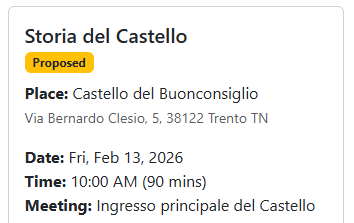
\includegraphics[width=\textwidth, keepaspectratio]{capitoli/immagini/p1.png}
        \caption{V1 (Prima)}
    \end{subfigure}
    \hfill
    \begin{subfigure}[b]{0.47\textwidth}
        \centering
        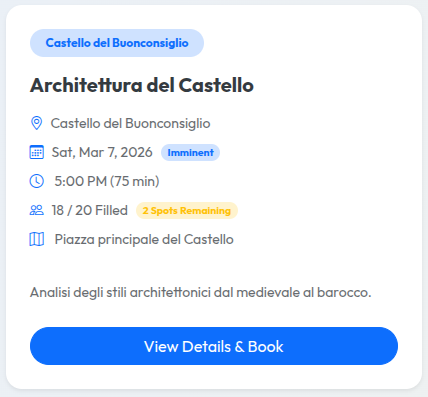
\includegraphics[width=\textwidth, keepaspectratio]{capitoli/immagini/v2/p3_v2.png}
        \caption{V2 (Dopo)}
    \end{subfigure}
    \caption{P.3 -- Badge stato: V1 (badge giallo "Proposed") vs V2 (badge blu "Upcoming").}
    \label{fig:det_p3}
\end{figure}

\noindent\textbf{P.4 -- Inconsistenza cromatica "Proposed"} \hfill \textit{Severità: 2}

Lo stesso stato compariva giallo in alcune viste e blu in altre. In V2 \texttt{bg-primary-subtle} è adottato uniformemente in tutte le schermate dell'applicativo.

\begin{figure}[H]
    \centering
    \begin{subfigure}[b]{0.47\textwidth}
        \centering
        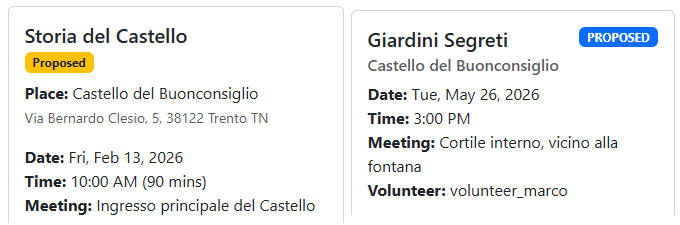
\includegraphics[width=\textwidth, keepaspectratio]{capitoli/immagini/p2.png}
        \caption{V1 (Prima)}
    \end{subfigure}
    \hfill
    \begin{subfigure}[b]{0.47\textwidth}
        \centering
        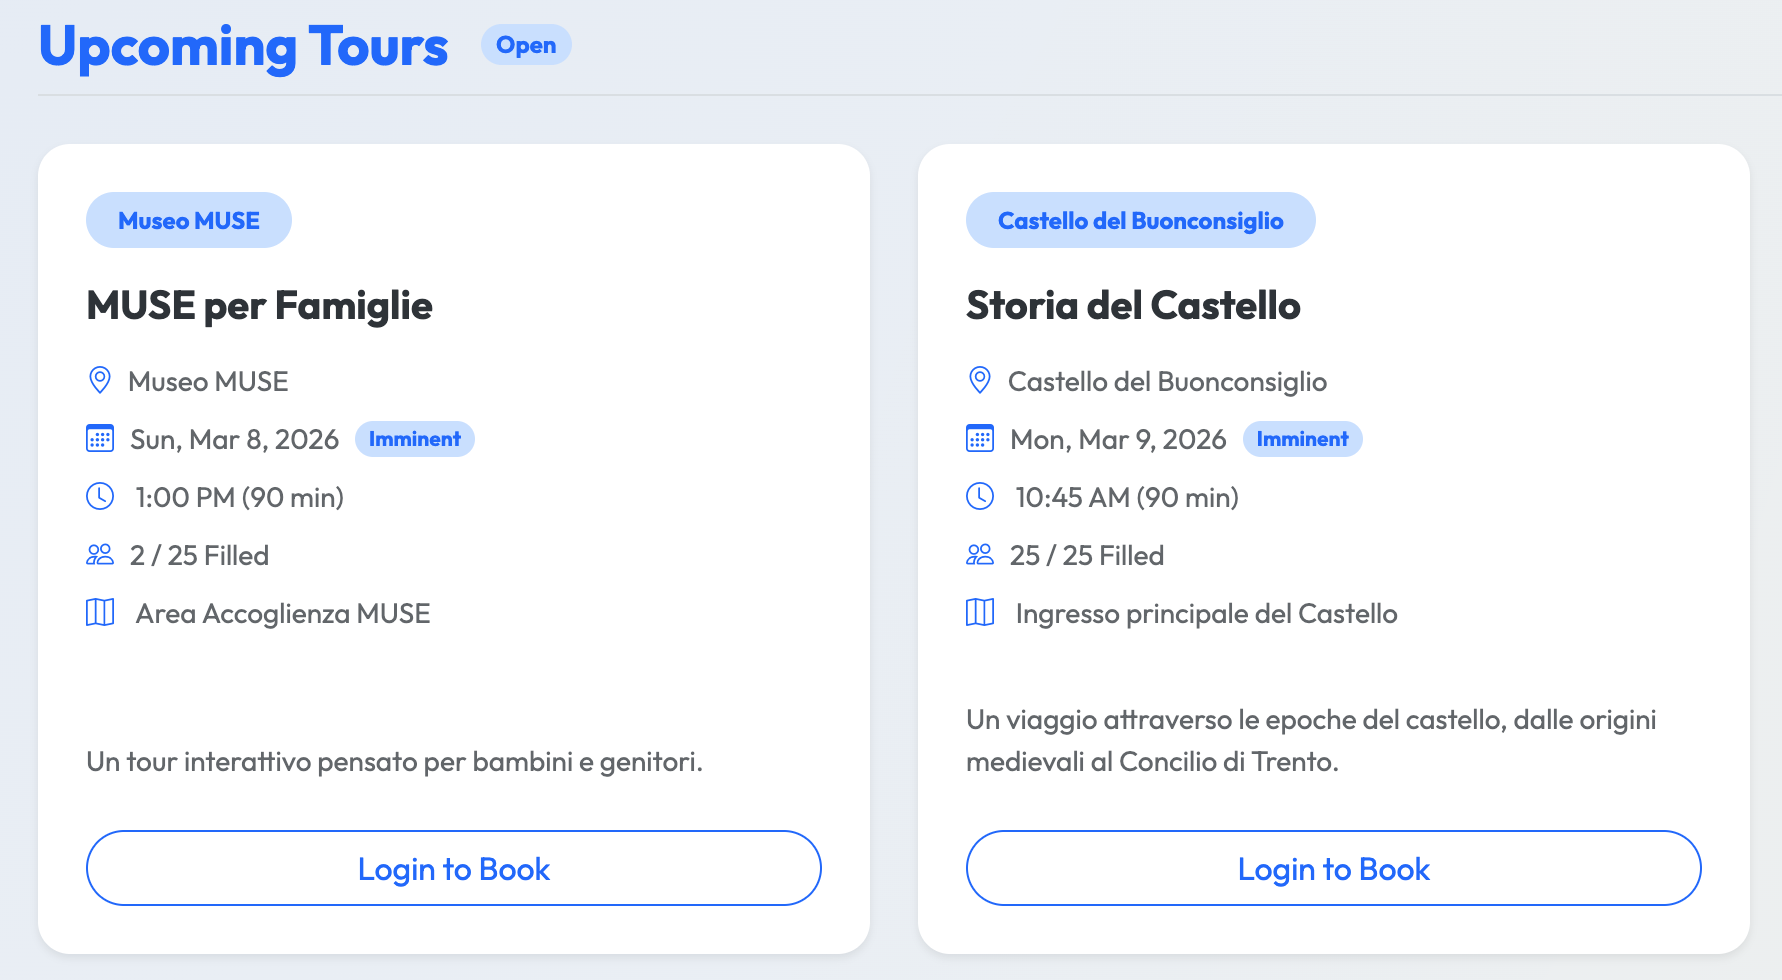
\includegraphics[width=\textwidth, keepaspectratio]{capitoli/immagini/v2/p4_v2.png}
        \caption{V2 (Dopo)}
    \end{subfigure}
    \caption{P.4 -- Inconsistenza cromatica: V1 (stesso stato, colori diversi) vs V2 (badge uniformi).}
    \label{fig:det_p4}
\end{figure}

\noindent\textbf{P.5 \& P.6 -- Chiarezza e stile nota pagamento} \hfill \textit{Severità: 2}

Il messaggio sulle modalità di pagamento era ambiguo e privo di enfasi visiva. In V2 ogni card mostra il prezzo esplicito (\textit{Free} o \textit{€X}) e la nota è presentata come banner \texttt{alert-warning} con icona, ad alto contrasto.

\begin{figure}[H]
    \centering
    \begin{subfigure}[b]{0.47\textwidth}
        \centering
        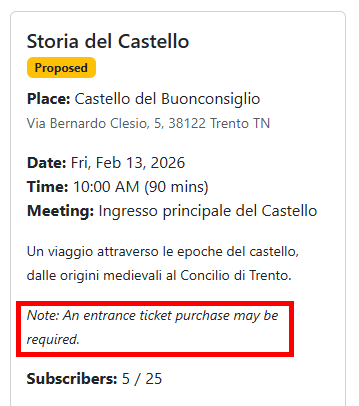
\includegraphics[width=\textwidth, keepaspectratio]{capitoli/immagini/p3.png}
        \caption{V1 (Prima)}
    \end{subfigure}
    \hfill
    \begin{subfigure}[b]{0.47\textwidth}
        \centering
        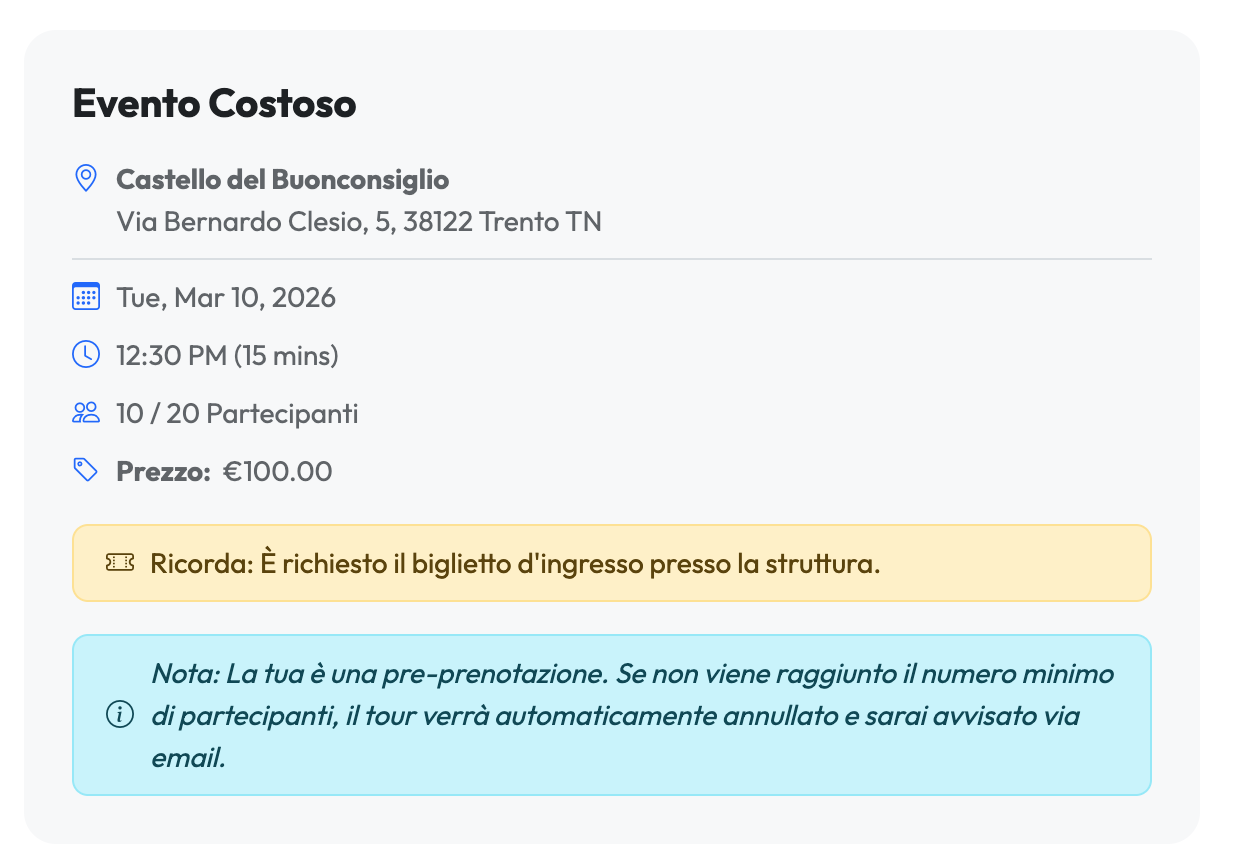
\includegraphics[width=\textwidth, keepaspectratio]{capitoli/immagini/v2/p6_v2.png}
        \caption{V2 (Dopo)}
    \end{subfigure}
    \caption{P.5/P.6 -- Nota pagamento: V1 (testo generico) vs V2 (prezzo esplicito e banner warning).}
    \label{fig:det_p5}
\end{figure}

\noindent\textbf{P.7 -- Ambiguità cromatica stati visita} \hfill \textit{Severità: 1}

"Confirmed" e "Complete" condividevano la stessa tinta verde. In V2 "Confirmed" mantiene \texttt{bg-success} (verde), "Complete" usa \texttt{bg-secondary} (grigio): la distinzione cromatica è immediata.

\begin{figure}[H]
    \centering
    \begin{subfigure}[b]{0.47\textwidth}
        \centering
        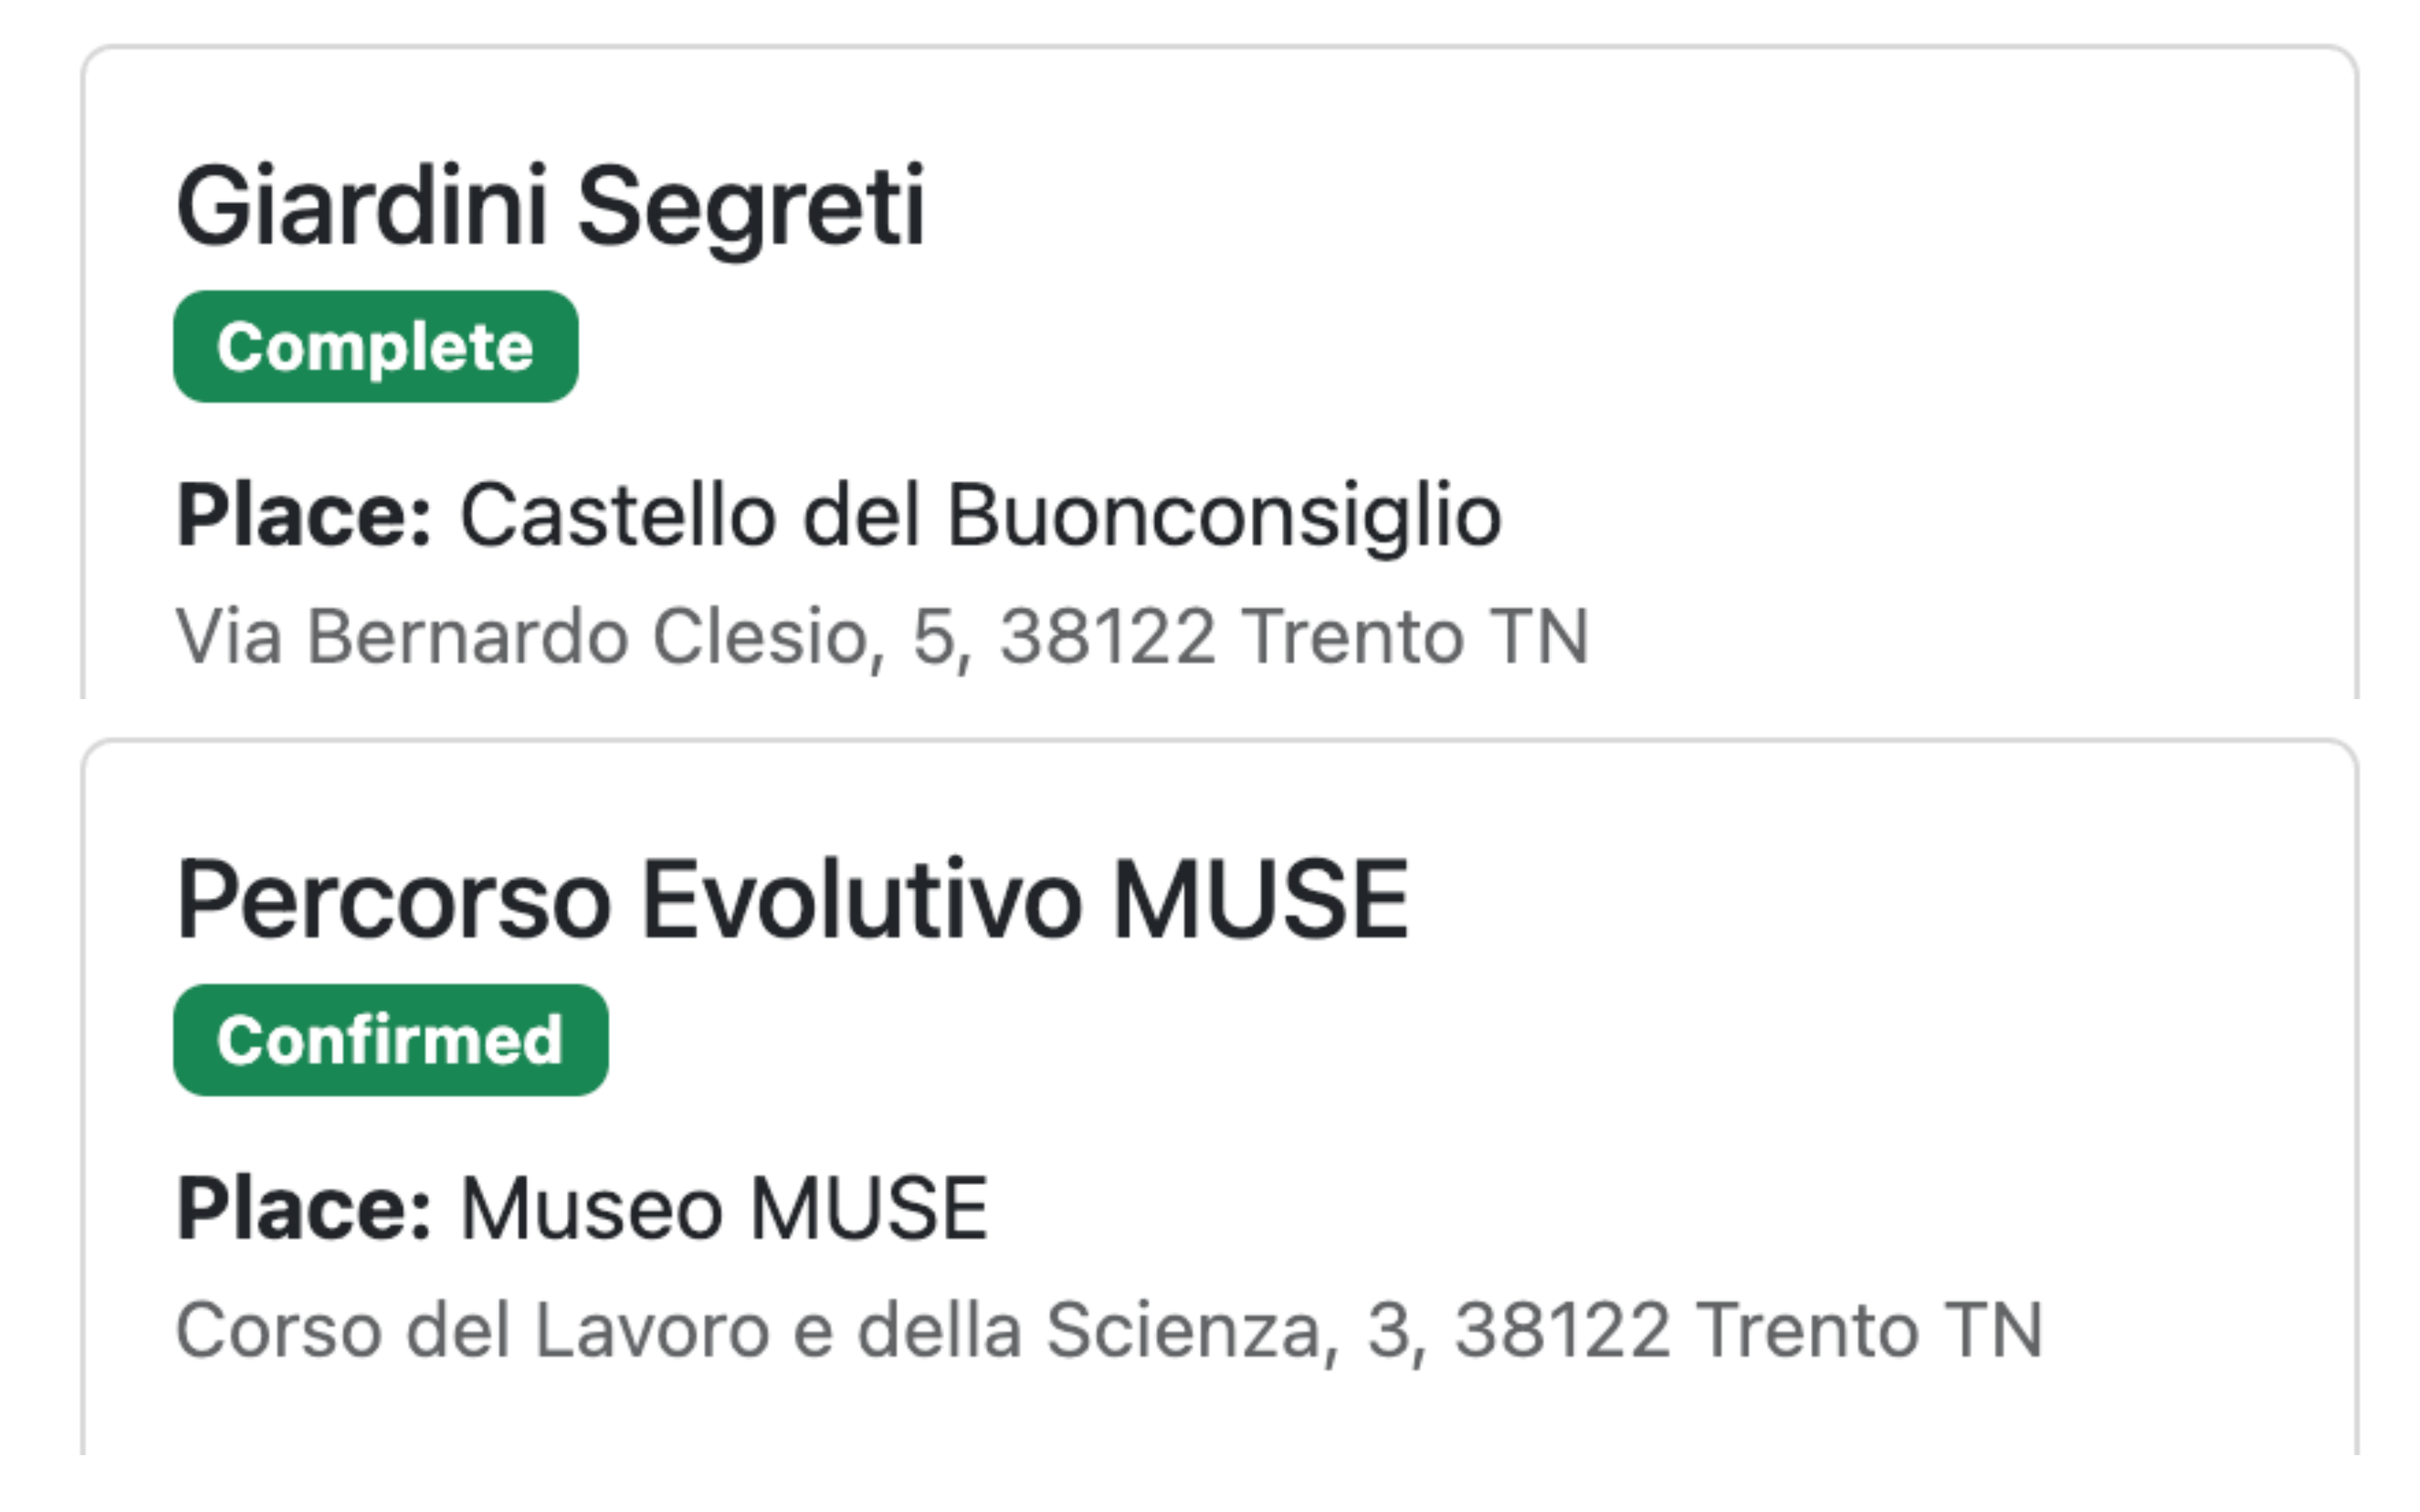
\includegraphics[width=\textwidth, keepaspectratio]{capitoli/immagini/p4.png}
        \caption{V1 (Prima)}
    \end{subfigure}
    \hfill
    \begin{subfigure}[b]{0.47\textwidth}
        \centering
        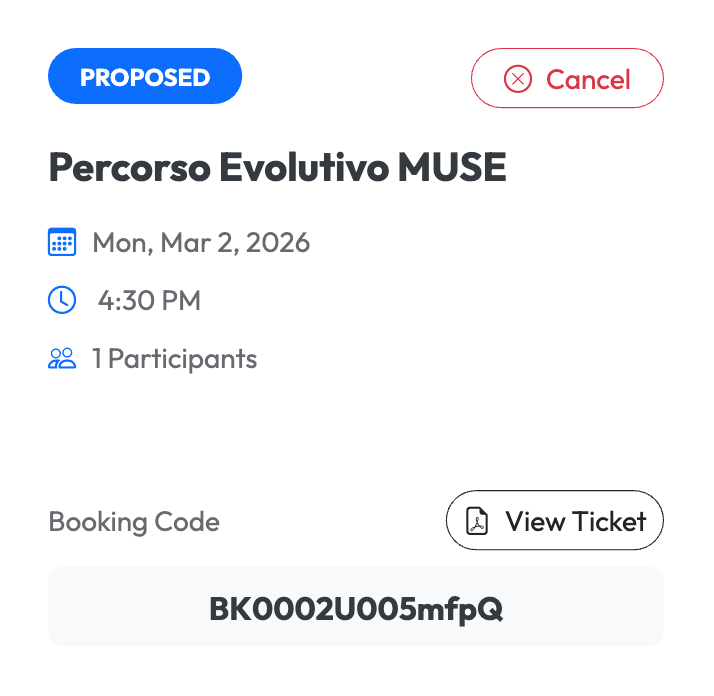
\includegraphics[width=\textwidth, keepaspectratio]{capitoli/immagini/v2/p7_v2.png}
        \caption{V2 (Dopo)}
    \end{subfigure}
    \caption{P.7 -- Ambiguità cromatica: V1 (badge identici) vs V2 (verde futuro, grigio passato).}
    \label{fig:det_p7}
\end{figure}

\noindent\textbf{P.8 -- Mancanza feedback disponibilità} \hfill \textit{Severità: 1}

Nessun indicatore visivo segnalava la saturazione delle visite. In V2 ogni card mostra il contatore "X/Y Filled" e il badge "Filling Fast" quando i posti scendono sotto soglia critica.

\begin{figure}[H]
    \centering
    \begin{subfigure}[b]{0.47\textwidth}
        \centering
        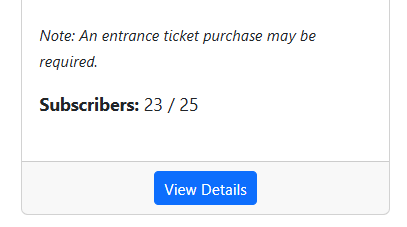
\includegraphics[width=\textwidth, keepaspectratio]{capitoli/immagini/p6.png}
        \caption{V1 (Prima)}
    \end{subfigure}
    \hfill
    \begin{subfigure}[b]{0.47\textwidth}
        \centering
        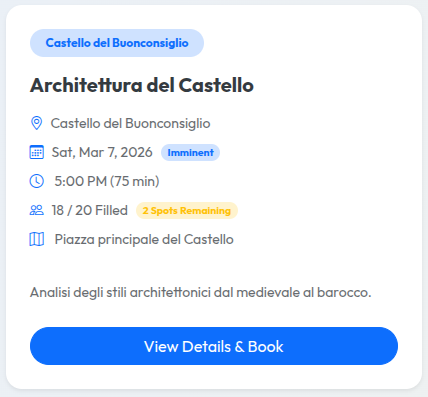
\includegraphics[width=\textwidth, keepaspectratio]{capitoli/immagini/v2/p3_v2.png}
        \caption{V2 (Dopo)}
    \end{subfigure}
    \caption{P.8 -- Feedback disponibilità: V1 (nessun indicatore) vs V2 (contatore posti e badge "Filling Fast").}
    \label{fig:det_p8}
\end{figure}

\noindent\textbf{P.9 -- Ridondanza "Visite confermate"} \hfill \textit{Severità: 1}

La sezione delle visite confermate risultava confusa. In V2 le sezioni "Upcoming" e "Your Confirmed" sono distinte con intestazioni esplicite che ne chiariscono il contenuto.

\begin{figure}[H]
    \centering
    \begin{subfigure}[b]{0.47\textwidth}
        \centering
        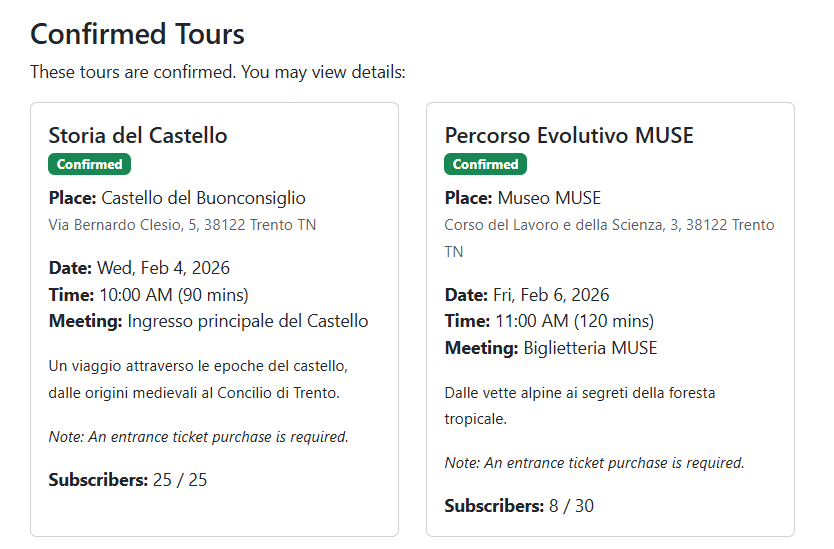
\includegraphics[width=\textwidth, keepaspectratio]{capitoli/immagini/p7.png}
        \caption{V1 (Prima)}
    \end{subfigure}
    \hfill
    \begin{subfigure}[b]{0.47\textwidth}
        \centering
        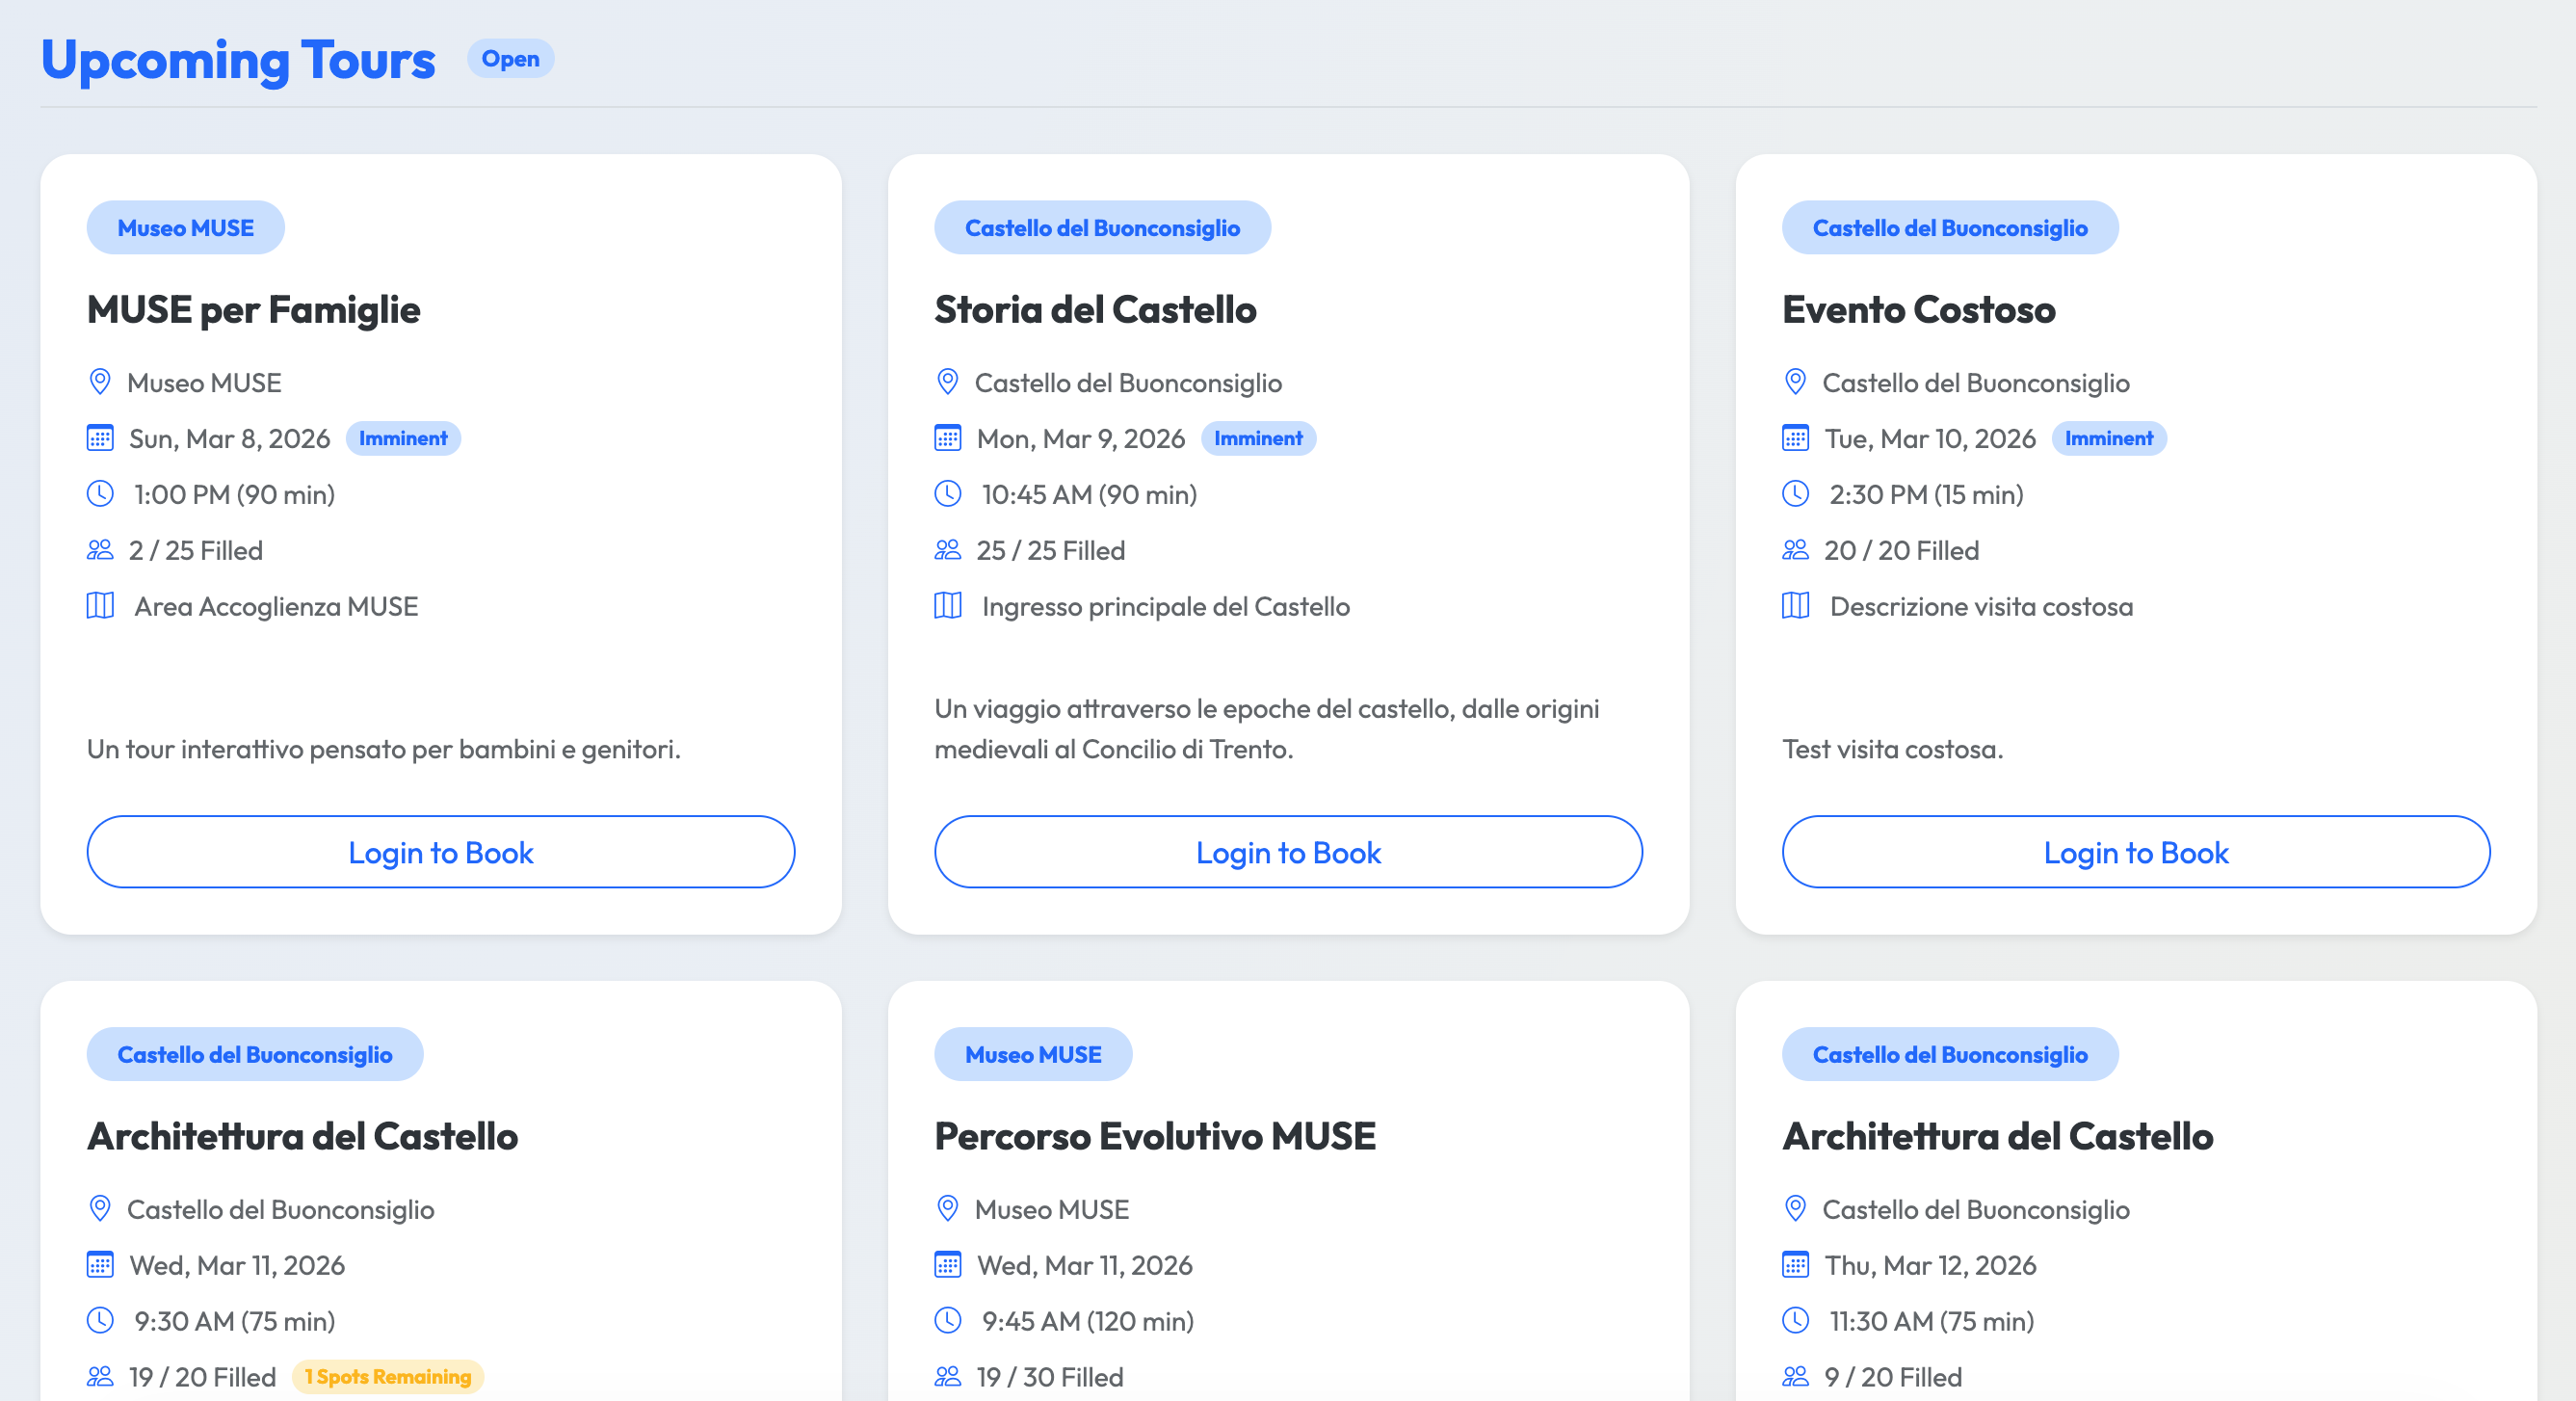
\includegraphics[width=\textwidth, keepaspectratio]{capitoli/immagini/v2/p9_v2.png}
        \caption{V2 (Dopo)}
    \end{subfigure}
    \caption{P.9 -- Sezioni homepage: V1 (struttura confusa) vs V2 (sezioni distinte con titoli chiari).}
    \label{fig:det_p9}
\end{figure}

\noindent\textbf{P.10 -- Area cliccabile limitata} \hfill \textit{Severità: 2}

L'accesso ai dettagli era vincolato al solo pulsante della card. In V2 l'intera card è cliccabile tramite \texttt{stretched-link} Bootstrap, con effetto hover visivo tramite classe \texttt{card-hover}.

\begin{figure}[H]
    \centering
    \begin{subfigure}[b]{0.47\textwidth}
        \centering
        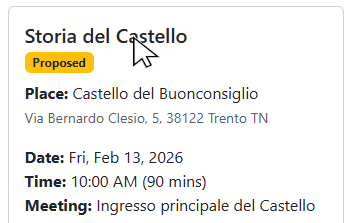
\includegraphics[width=\textwidth, keepaspectratio]{capitoli/immagini/p8.png}
        \caption{V1 (Prima)}
    \end{subfigure}
    \hfill
    \begin{subfigure}[b]{0.47\textwidth}
        \centering
        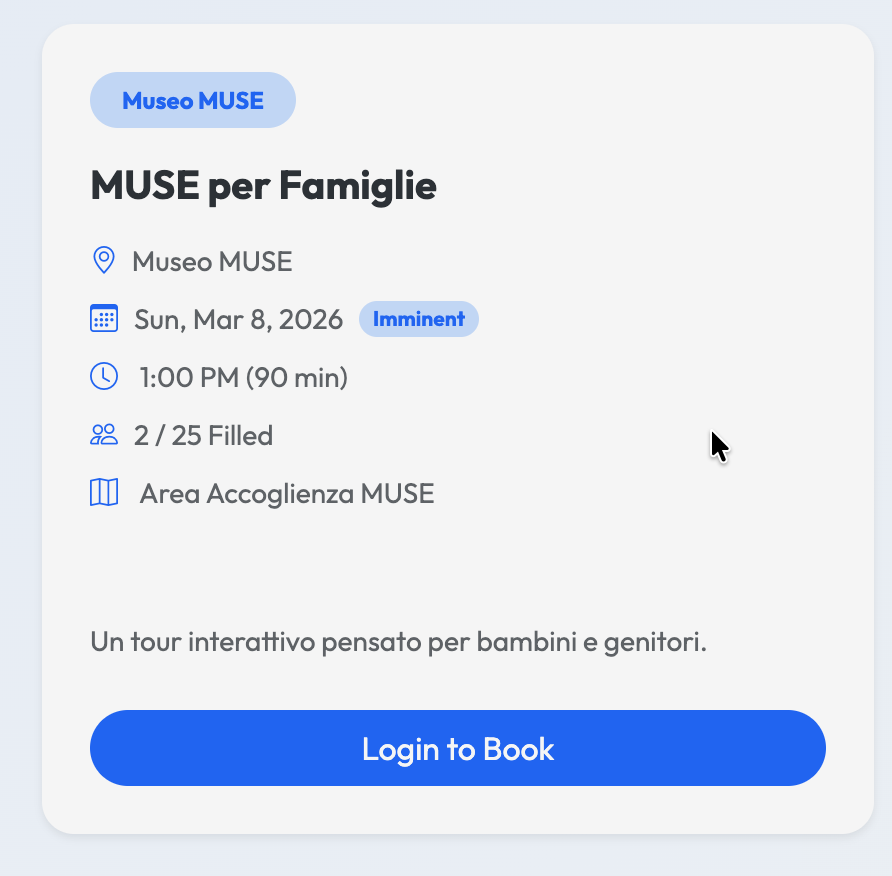
\includegraphics[width=\textwidth, keepaspectratio]{capitoli/immagini/v2/p10_v2.png}
        \caption{V2 (Dopo)}
    \end{subfigure}
    \caption{P.10 -- Area cliccabile: V1 (solo bottone) vs V2 (intera card interattiva con hover).}
    \label{fig:det_p10}
\end{figure}

\noindent\textbf{P.11 -- Gerarchia visiva debole} \hfill \textit{Severità: 1}

La gerarchia tipografica era appiattita. In V2 è implementata una scala chiara: \texttt{display-4} per il titolo hero, \texttt{h3} per le sezioni, \texttt{h5} per i sottotitoli delle card.

\begin{figure}[H]
    \centering
    \begin{subfigure}[b]{0.47\textwidth}
        \centering
        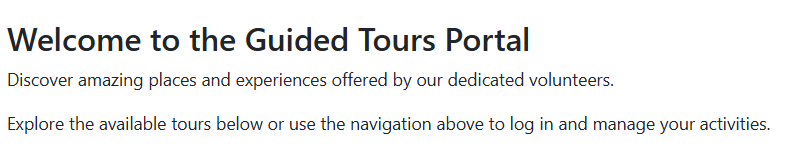
\includegraphics[width=\textwidth, keepaspectratio]{capitoli/immagini/p9.png}
        \caption{V1 (Prima)}
    \end{subfigure}
    \hfill
    \begin{subfigure}[b]{0.47\textwidth}
        \centering
        
\includegraphics[width=\textwidth, keepaspectratio]{capitoli/immagini/v2/p11_v2.png}
        \caption{V2 (Dopo)}
    \end{subfigure}
    \caption{P.11 -- Gerarchia visiva: V1 (gerarchia debole) vs V2 (tipografia \texttt{display-4} con forte contrasto).}
    \label{fig:det_p11}
\end{figure}

\noindent\textbf{P.12 -- Assenza shortcut area personale} \hfill \textit{Severità: 1}

Dalla homepage mancava un accesso diretto alla propria area personale. In V2 l'hero section include, per gli utenti autenticati come Customer, un bottone "My Dashboard" per raggiungerla in un click.

\begin{figure}[H]
    \centering
    \begin{subfigure}[b]{0.47\textwidth}
        \centering
        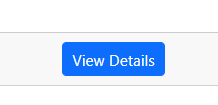
\includegraphics[width=\textwidth, keepaspectratio]{capitoli/immagini/p10.png}
        \caption{V1 (Prima)}
    \end{subfigure}
    \hfill
    \begin{subfigure}[b]{0.47\textwidth}
        \centering
        
\includegraphics[width=\textwidth, keepaspectratio]{capitoli/immagini/v2/p12_v2.png}
        \caption{V2 (Dopo)}
    \end{subfigure}
    \caption{P.12 -- Shortcut area personale: V1 (nessun accesso rapido) vs V2 (bottone "My Dashboard" nell'hero).}
    \label{fig:det_p12}
\end{figure}

\subsection{Footer e Navbar}

\noindent\textbf{P.13 -- Incoerenza linguistica} \hfill \textit{Severità: 1}

Il footer conteneva la dicitura italiana "Sito di visite guidate" in un'interfaccia altrimenti in inglese. In V2 l'intero footer è riscritto in inglese.

\begin{figure}[H]
    \centering
    \begin{subfigure}[b]{0.47\textwidth}
        \centering
        
\includegraphics[width=\textwidth, keepaspectratio]{capitoli/immagini/p12.png}
        \caption{V1 (Prima)}
    \end{subfigure}
    \hfill
    \begin{subfigure}[b]{0.47\textwidth}
        \centering
        
\includegraphics[width=\textwidth, keepaspectratio]{capitoli/immagini/v2/p13_v2.png}
        \caption{V2 (Dopo)}
    \end{subfigure}
    \caption{P.13 -- Incoerenza linguistica: V1 (testo italiano nel footer) vs V2 (footer interamente in inglese).}
    \label{fig:det_p13}
\end{figure}

\noindent\textbf{P.35 -- Email non cliccabili} \hfill \textit{Severità: 2}

Gli indirizzi email nel footer non erano cliccabili nonostante l'aspetto da link. In V2 sono avvolti da tag \texttt{<a href="mailto:...">} e stilizzati coerentemente.

\begin{figure}[H]
    \centering
    \begin{subfigure}[b]{0.47\textwidth}
        \centering
        
\includegraphics[width=\textwidth, keepaspectratio]{capitoli/immagini/p33.png}
        \caption{V1 (Prima)}
    \end{subfigure}
    \hfill
    \begin{subfigure}[b]{0.47\textwidth}
        \centering
        
\includegraphics[width=\textwidth, keepaspectratio]{capitoli/immagini/v2/p35_v2.png}
        \caption{V2 (Dopo)}
    \end{subfigure}
    \caption{P.35 -- Email cliccabili: V1 (testo statico) vs V2 (link \texttt{mailto} attivi).}
    \label{fig:det_p35}
\end{figure}

\subsection{Autenticazione (Login e Register)}

\noindent\textbf{P.15 -- Mancanza toggle visibilità password} \hfill \textit{Severità: 1}

L'assenza di un toggle per visualizzare la password aumentava la probabilità di errori di digitazione. In V2 è presente un'icona occhio con script \texttt{showPassword()} nelle pagine Login e Register.

\begin{figure}[H]
    \centering
    \begin{subfigure}[b]{0.47\textwidth}
        \centering
        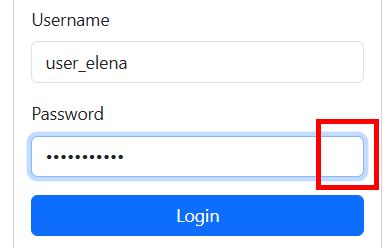
\includegraphics[width=\textwidth, keepaspectratio]{capitoli/immagini/p11.png}
        \caption{V1 (Prima)}
    \end{subfigure}
    \hfill
    \begin{subfigure}[b]{0.47\textwidth}
        \centering
        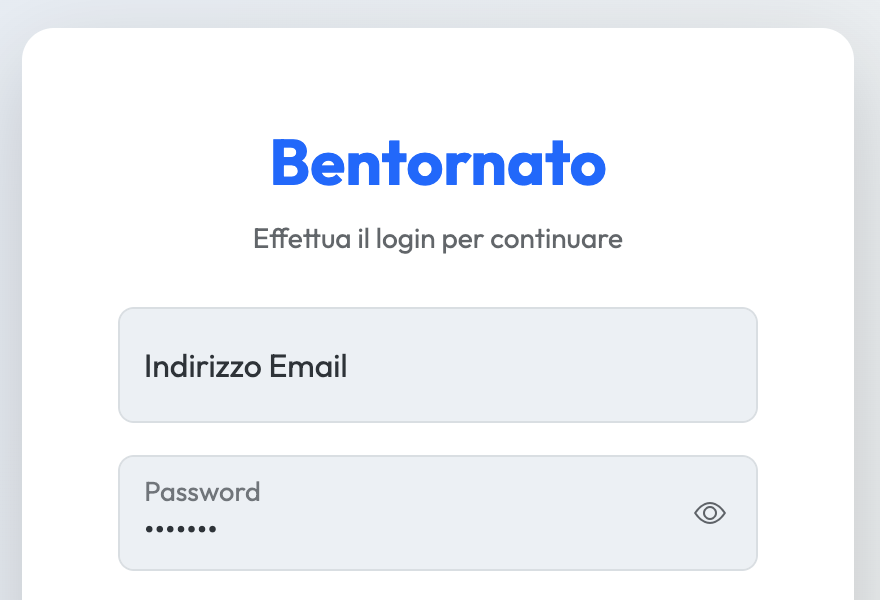
\includegraphics[width=\textwidth, keepaspectratio]{capitoli/immagini/v2/p15_v2.png}
        \caption{V2 (Dopo)}
    \end{subfigure}
    \caption{P.15 -- Toggle password: V1 (campo senza icona) vs V2 (icona occhio attiva).}
    \label{fig:det_p15}
\end{figure}

\noindent\textbf{P.16 \& P.17 -- Navigazione ambigua e ridondanza ruoli (Login)} \hfill \textit{Severità: 1}

La pagina di login presentava link multipli e testo ridondante sui ruoli. In V2 rimane un solo link "Create an Account" e il testo è ridotto all'essenziale.

\begin{figure}[H]
    \centering
    \begin{subfigure}[b]{0.47\textwidth}
        \centering
        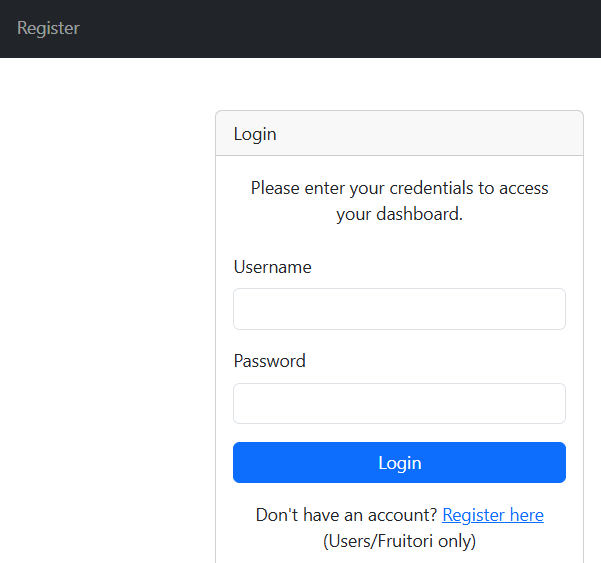
\includegraphics[width=\textwidth, keepaspectratio]{capitoli/immagini/p14.png}
        \caption{V1 (Prima)}
    \end{subfigure}
    \hfill
    \begin{subfigure}[b]{0.47\textwidth}
        \centering
        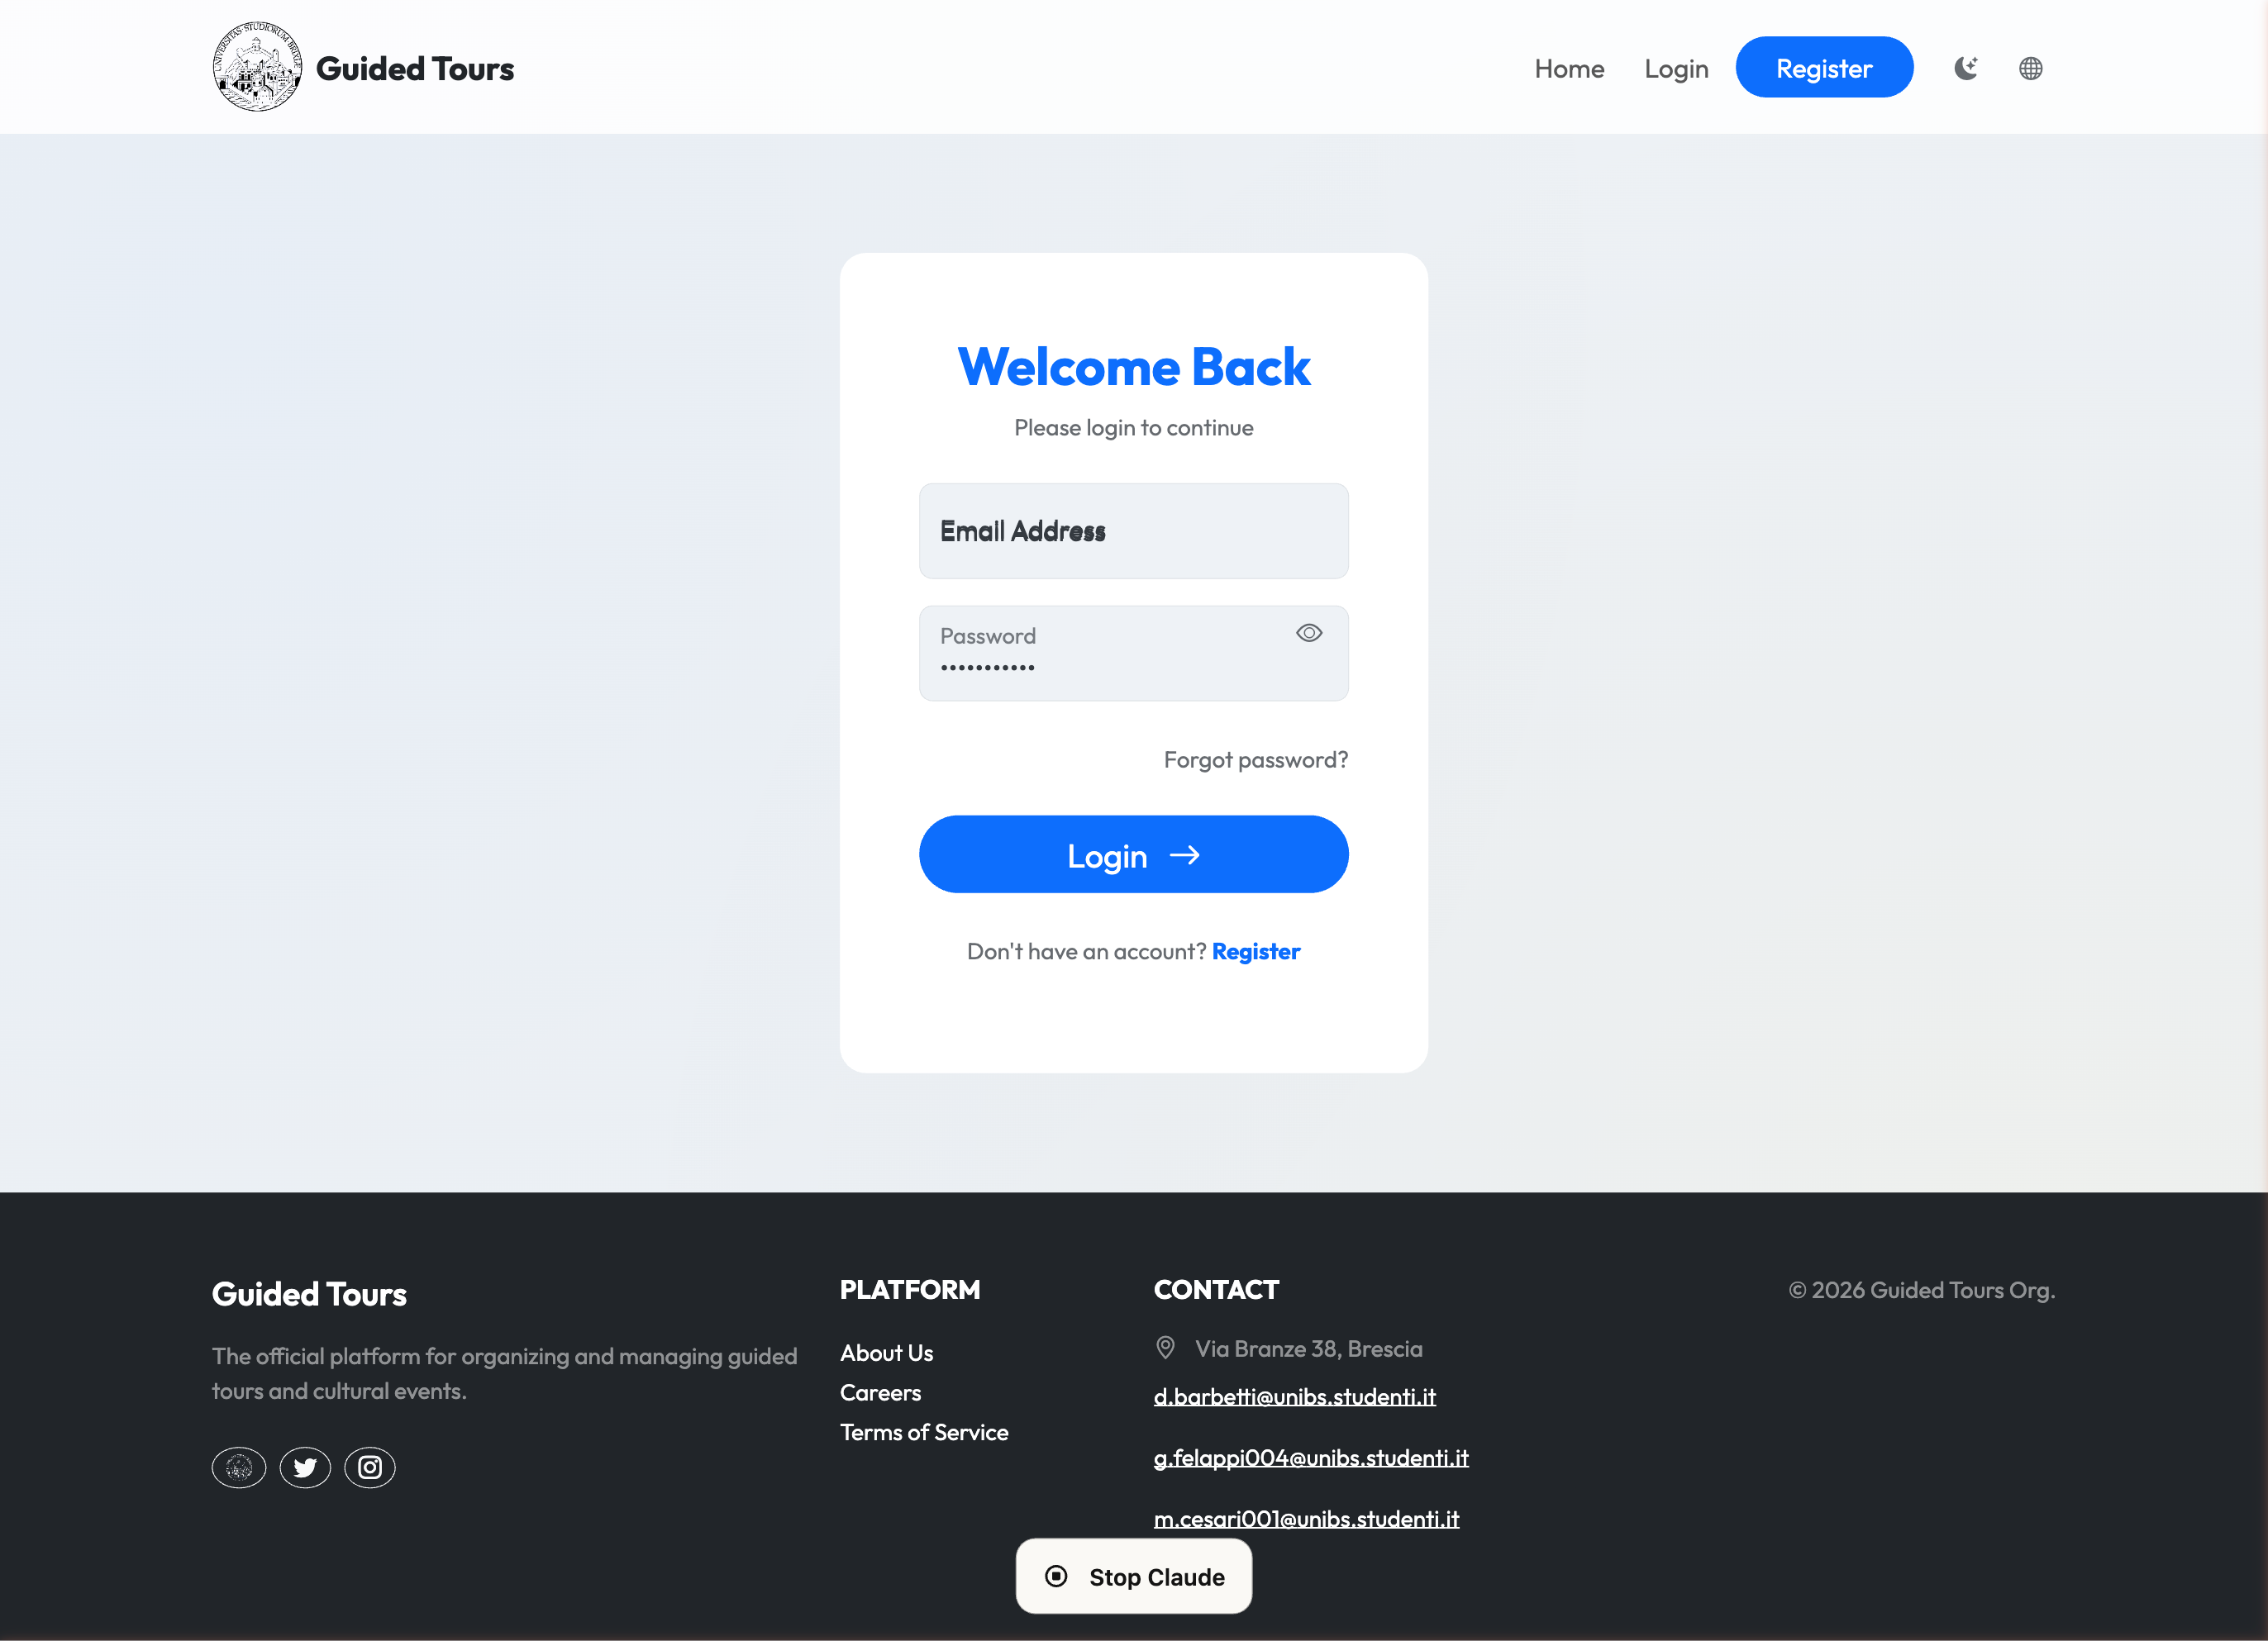
\includegraphics[width=\textwidth, keepaspectratio]{capitoli/immagini/v2/p16_v2.png}
        \caption{V2 (Dopo)}
    \end{subfigure}
    \caption{P.16/P.17 -- Login: V1 (link multipli e testo ridondante) vs V2 (form pulito con link unico).}
    \label{fig:det_p16}
\end{figure}

\noindent\textbf{P.18 -- Feedback errore non user-friendly} \hfill \textit{Severità: 1}

I messaggi di errore in caso di credenziali errate erano tecnici e poco comprensibili. In V2 sono presentati tramite Toast Notifications con testo chiaro e contestuale.

\begin{figure}[H]
    \centering
    \begin{subfigure}[b]{0.47\textwidth}
        \centering
        
\includegraphics[width=\textwidth, keepaspectratio]{capitoli/immagini/p16.png}
        \caption{V1 (Prima)}
    \end{subfigure}
    \hfill
    \begin{subfigure}[b]{0.47\textwidth}
        \centering
        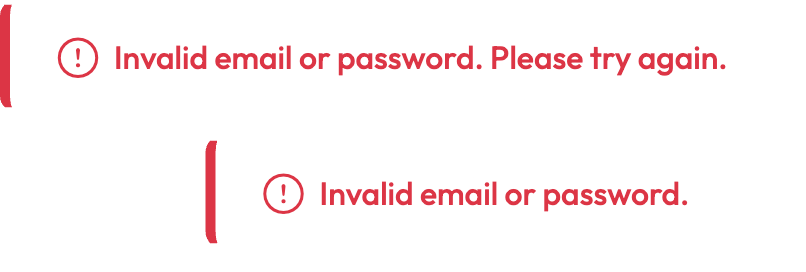
\includegraphics[width=\textwidth, keepaspectratio]{capitoli/immagini/v2/p18_v2.png}
        \caption{V2 (Dopo)}
    \end{subfigure}
    \caption{P.18 -- Feedback errore: V1 (messaggio tecnico) vs V2 (Toast Notification chiara).}
    \label{fig:det_p18}
\end{figure}

\noindent\textbf{P.19 -- Assenza recupero password} \hfill \textit{Severità: 3}

La mancanza di un meccanismo di recupero delle credenziali bloccava l'utente in caso di smarrimento. In V2 è implementata una pagina "Forgot Password" con reset tramite link inviato via email.

\begin{figure}[H]
    \centering
    \begin{subfigure}[b]{0.47\textwidth}
        \centering
        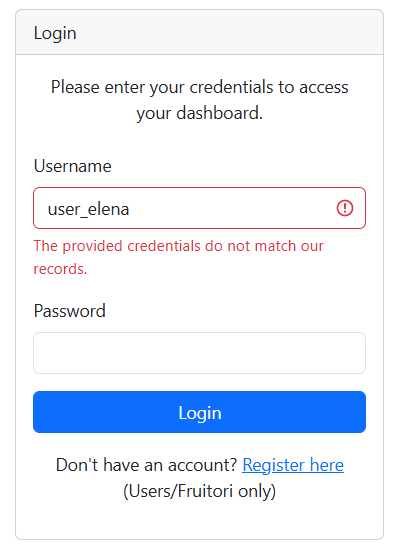
\includegraphics[width=\textwidth, keepaspectratio]{capitoli/immagini/p17.png}
        \caption{V1 (Prima)}
    \end{subfigure}
    \hfill
    \begin{subfigure}[b]{0.47\textwidth}
        \centering
        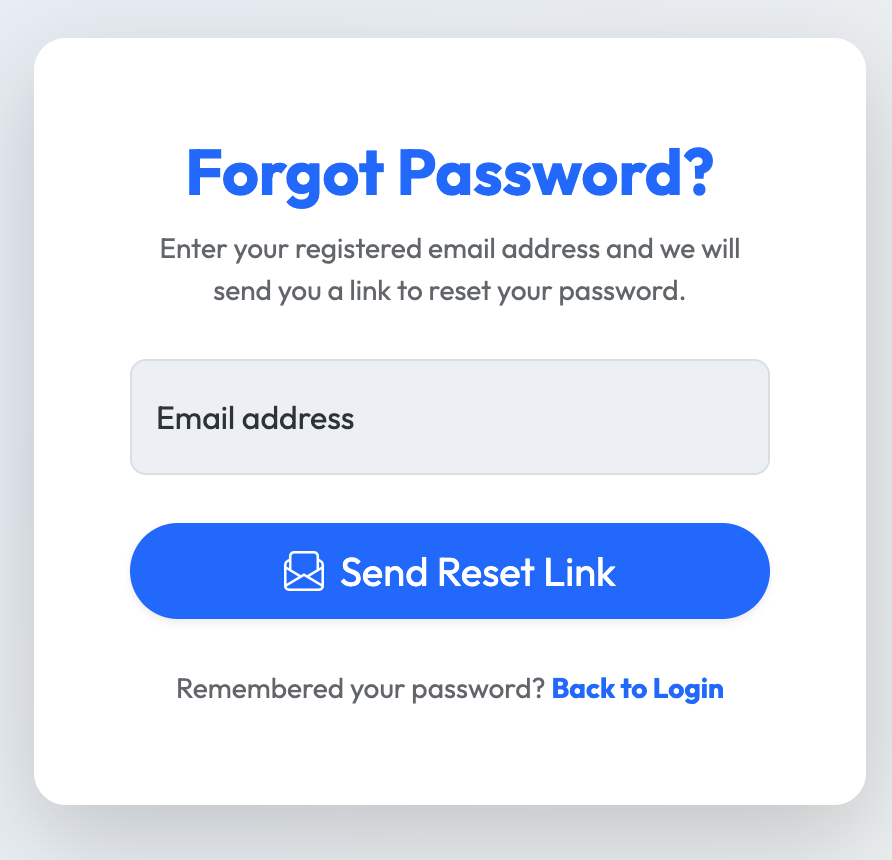
\includegraphics[width=\textwidth, keepaspectratio]{capitoli/immagini/v2/p19_v2.png}
        \caption{V2 (Dopo)}
    \end{subfigure}
    \caption{P.19 -- Recupero password: V1 (nessun link) vs V2 (pagina "Forgot Password" con reset via email).}
    \label{fig:det_p19}
\end{figure}

\noindent\textbf{P.20 -- Carico cognitivo posti disponibili} \hfill \textit{Severità: 2}

L'utente doveva calcolare autonomamente i posti liberi nel form di prenotazione. In V2 il campo mostra esplicitamente "(X spots remaining)" in tempo reale.

\begin{figure}[H]
    \centering
    \begin{subfigure}[b]{0.42\textwidth}
        \centering
        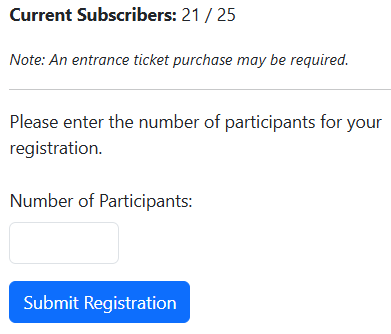
\includegraphics[width=\textwidth, keepaspectratio]{capitoli/immagini/p18.png}
        \caption{V1 (Prima)}
    \end{subfigure}
    \hfill
    \begin{subfigure}[b]{0.4\textwidth}
        \centering
        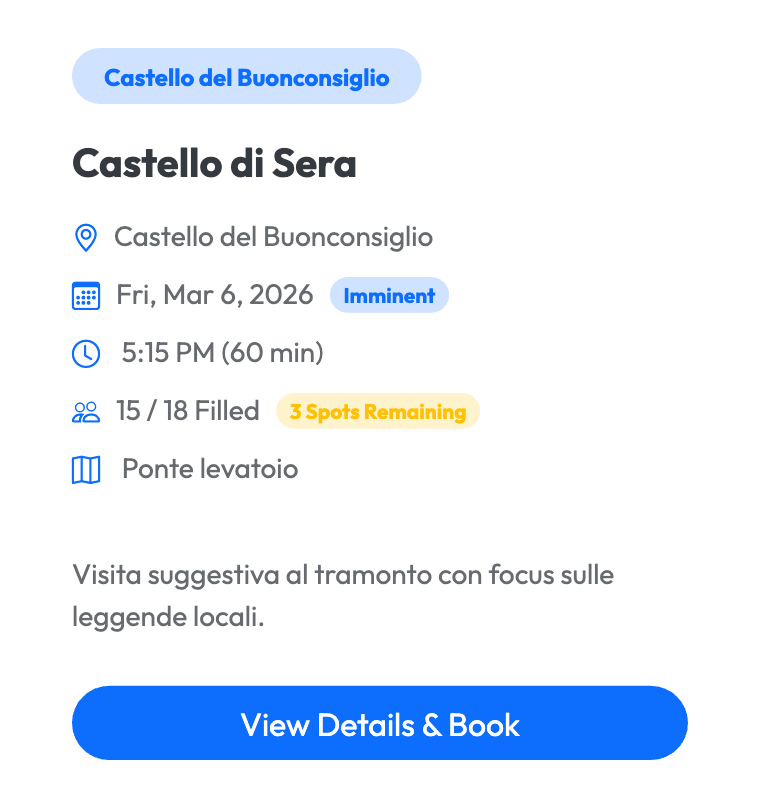
\includegraphics[width=\textwidth, keepaspectratio]{capitoli/immagini/v2/p20_v2.png}
        \caption{V2 (Dopo)}
    \end{subfigure}
    \caption{P.20 -- Posti disponibili: V1 (nessun indicatore) vs V2 (contatore "(X spots remaining)" esplicito).}
    \label{fig:det_p20}
\end{figure}

\noindent\textbf{P.21 \& P.22 -- Ridondanza informativa Register} \hfill \textit{Severità: 1}

La pagina di registrazione aveva link multipli verso il login e spiegazioni dei ruoli non necessarie. In V2 il form è semplificato: un solo link "Already have an account? Login" e nessuna descrizione dei ruoli.

\begin{figure}[H]
    \centering
    \begin{subfigure}[b]{0.47\textwidth}
        \centering
        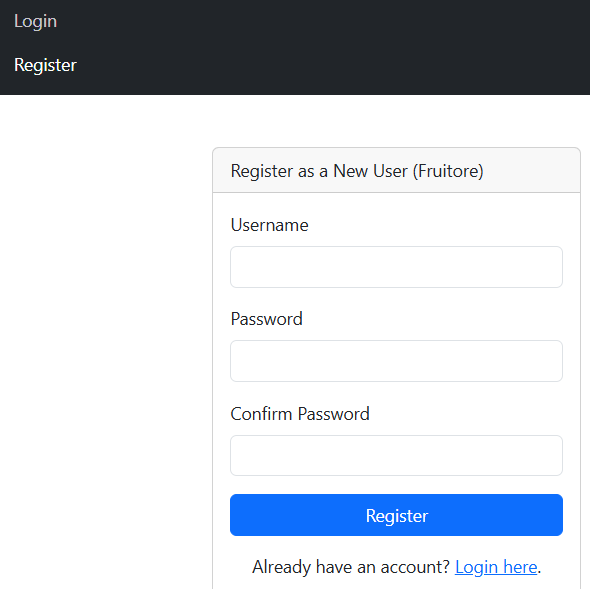
\includegraphics[width=\textwidth, keepaspectratio]{capitoli/immagini/p19.png}
        \caption{V1 (Prima)}
    \end{subfigure}
    \hfill
    \begin{subfigure}[b]{0.47\textwidth}
        \centering
        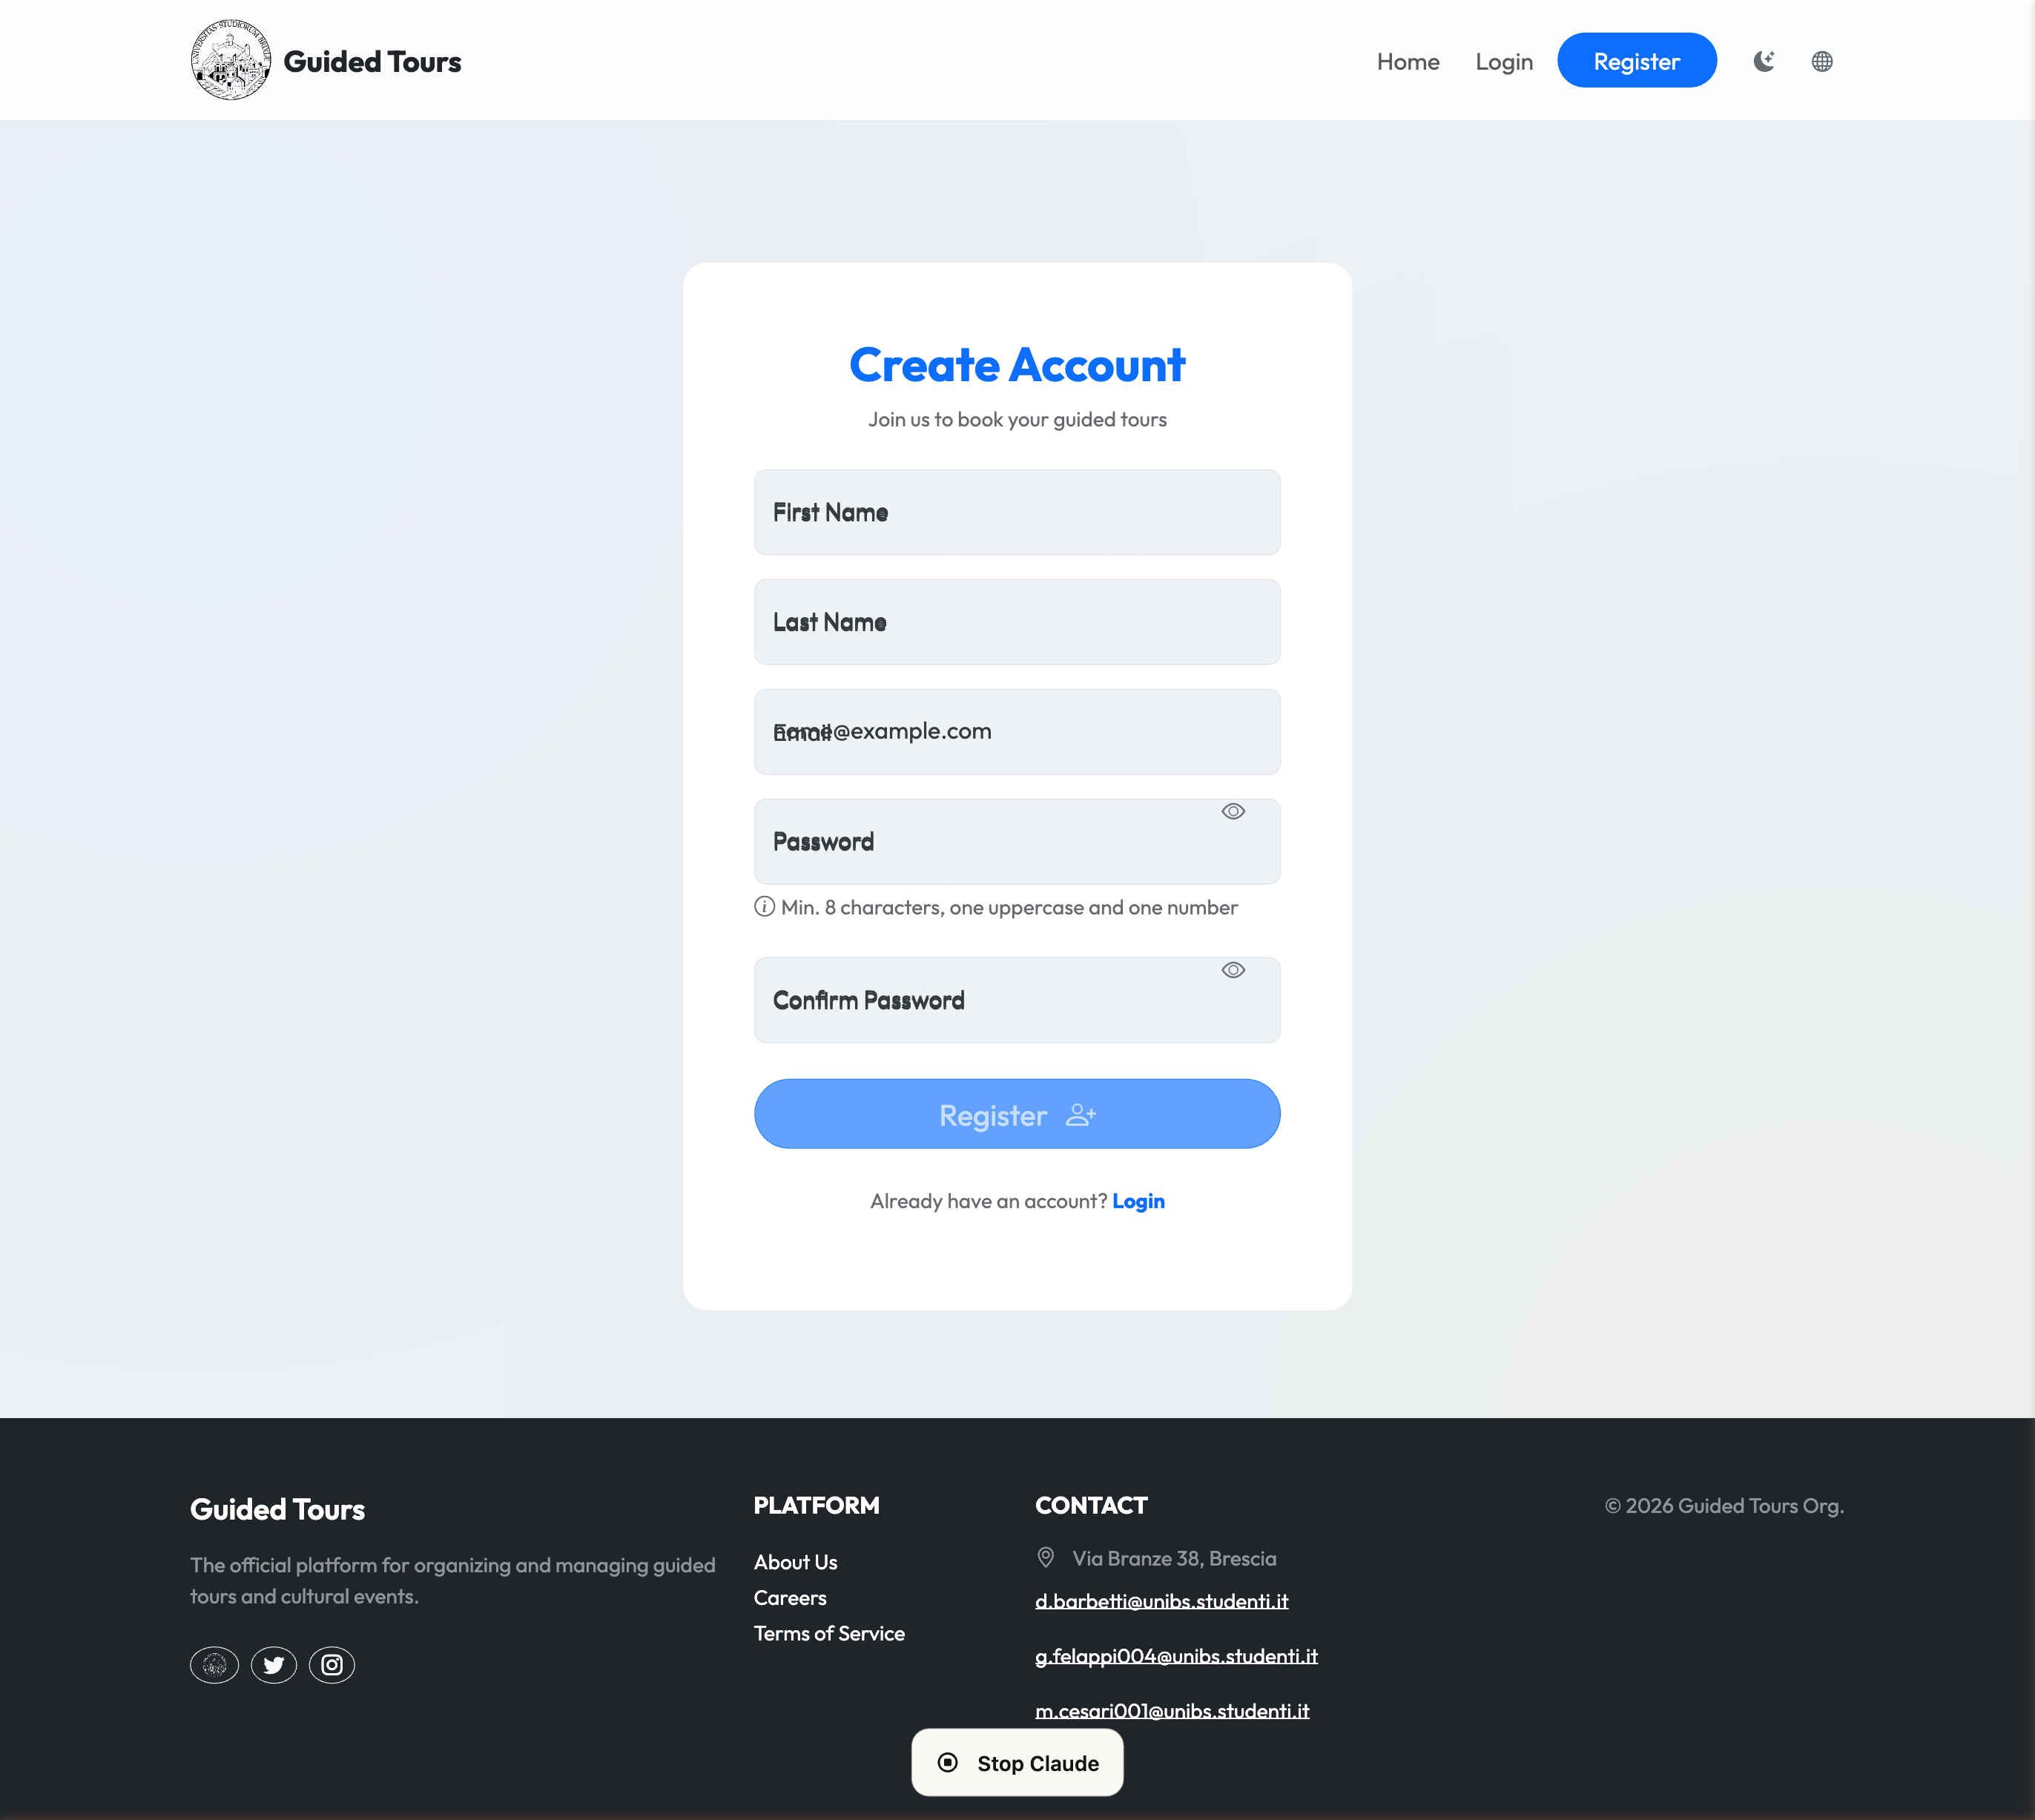
\includegraphics[width=\textwidth, keepaspectratio]{capitoli/immagini/v2/p21_v2.png}
        \caption{V2 (Dopo)}
    \end{subfigure}
    \caption{P.21/P.22 -- Register: V1 (link ridondanti e testo sui ruoli) vs V2 (form essenziale).}
    \label{fig:det_p21}
\end{figure}

\noindent\textbf{P.23 -- Validazione tardiva input} \hfill \textit{Severità: 2}

La validazione della password avveniva solo al submit. In V2 script JavaScript forniscono feedback visivo in tempo reale durante la digitazione: lunghezza minima e corrispondenza tra i due campi.

\begin{figure}[H]
    \centering
    \begin{subfigure}[b]{0.47\textwidth}
        \centering
        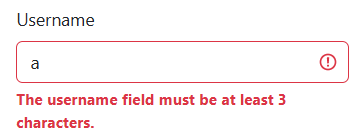
\includegraphics[width=\textwidth, keepaspectratio]{capitoli/immagini/p21.png}
        \caption{V1 (Prima)}
    \end{subfigure}
    \hfill
    \begin{subfigure}[b]{0.47\textwidth}
        \centering
        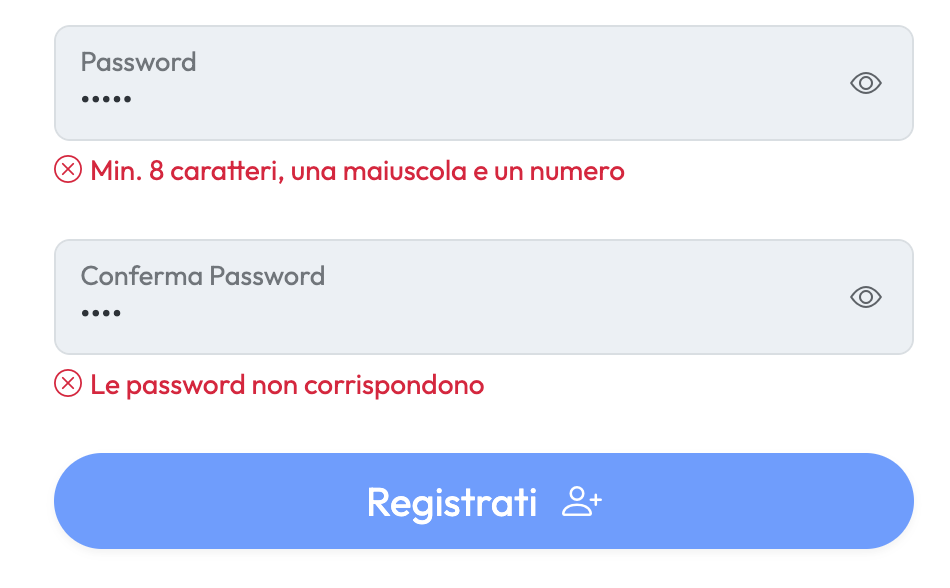
\includegraphics[width=\textwidth, keepaspectratio]{capitoli/immagini/v2/p23_v2.png}
        \caption{V2 (Dopo)}
    \end{subfigure}
    \caption{P.23 -- Validazione live: V1 (nessun feedback) vs V2 (indicatori real-time di lunghezza e match password).}
    \label{fig:det_p23}
\end{figure}

\subsection{Dashboard Fruitore}

\noindent\textbf{P.24 -- Visibilità "Booking code"} \hfill \textit{Severità: 1}

Il codice di prenotazione era presentato senza enfasi visiva. In V2 è visualizzato in font monospaziato bold con etichetta "Booking Code" esplicita.

\begin{figure}[H]
    \centering
    \begin{subfigure}[b]{0.47\textwidth}
        \centering
        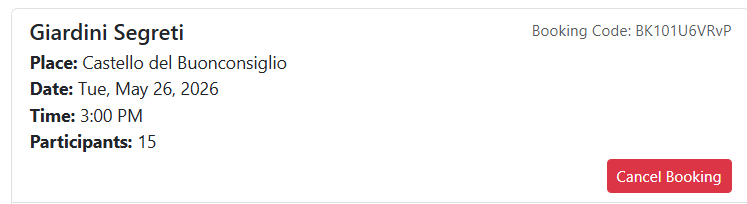
\includegraphics[width=\textwidth, keepaspectratio]{capitoli/immagini/p22.png}
        \caption{V1 (Prima)}
    \end{subfigure}
    \hfill
    \begin{subfigure}[b]{0.47\textwidth}
        \centering
        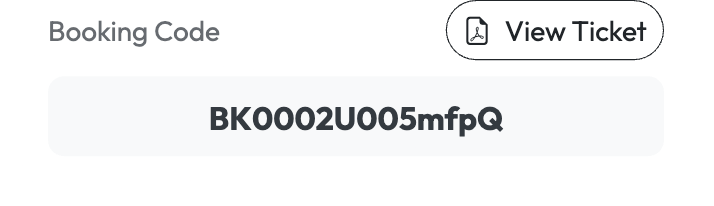
\includegraphics[width=\textwidth, keepaspectratio]{capitoli/immagini/v2/p24_v2.png}
        \caption{V2 (Dopo)}
    \end{subfigure}
    \caption{P.24 -- Booking code: V1 (testo generico) vs V2 (font monospaziato bold con etichetta esplicita).}
    \label{fig:det_p24}
\end{figure}

\noindent\textbf{P.25 -- Ambiguità etichetta "Participant"} \hfill \textit{Severità: 2}

L'etichetta non chiariva se indicasse il gruppo dell'utente o il totale della visita. In V2 è standardizzata in "X Participants".

\begin{figure}[H]
    \centering
    \begin{subfigure}[b]{0.47\textwidth}
        \centering
        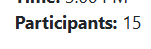
\includegraphics[width=\textwidth, keepaspectratio]{capitoli/immagini/p23.png}
        \caption{V1 (Prima)}
    \end{subfigure}
    \hfill
    \begin{subfigure}[b]{0.47\textwidth}
        \centering
        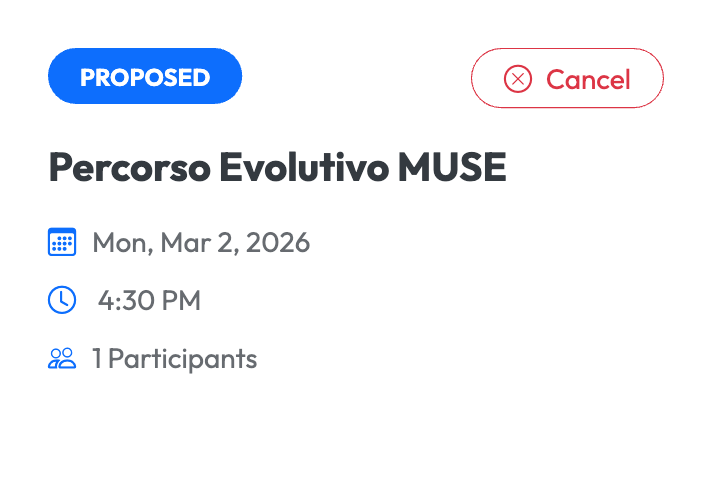
\includegraphics[width=\textwidth, keepaspectratio]{capitoli/immagini/v2/p25_v2.png}
        \caption{V2 (Dopo)}
    \end{subfigure}
    \caption{P.25 -- Etichetta partecipanti: V1 (ambigua) vs V2 (standardizzata "X Participants").}
    \label{fig:det_p25}
\end{figure}

\noindent\textbf{P.26 -- Affordance ingannevole "My Booking"} \hfill \textit{Severità: 2}

Il menu a tendina suggeriva interattività che non portava ad azioni utili. In V2 è sostituito da un bottone esplicito "Cancel Booking" con modale di conferma.

\begin{figure}[H]
    \centering
    \begin{subfigure}[b]{0.47\textwidth}
        \centering
        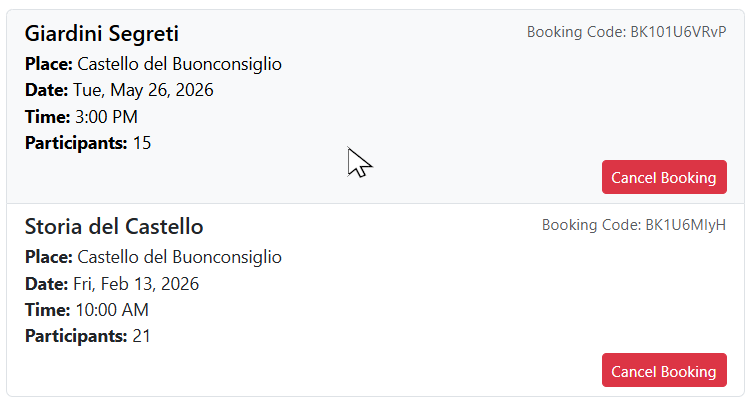
\includegraphics[width=\textwidth, keepaspectratio]{capitoli/immagini/p24.png}
        \caption{V1 (Prima)}
    \end{subfigure}
    \hfill
    \begin{subfigure}[b]{0.47\textwidth}
        \centering
        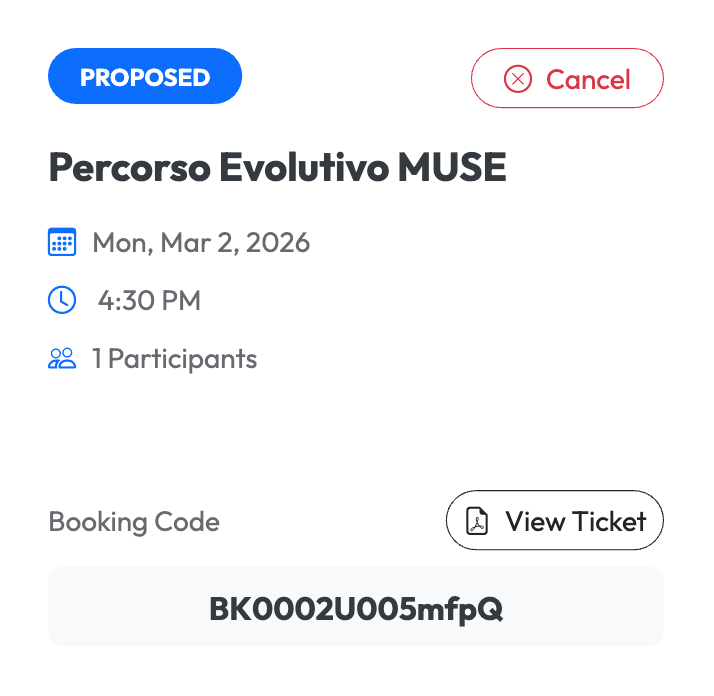
\includegraphics[width=\textwidth, keepaspectratio]{capitoli/immagini/v2/p26_v2.png}
        \caption{V2 (Dopo)}
    \end{subfigure}
    \caption{P.26 -- Affordance: V1 (menu ambiguo) vs V2 (bottone "Cancel Booking" con modale).}
    \label{fig:det_p26}
\end{figure}

\noindent\textbf{P.27 -- Stile pulsante eliminazione} \hfill \textit{Severità: 1}

Il bottone di cancellazione non comunicava la pericolosità dell'azione. In V2 adotta \texttt{btn-danger} con testo rosso, coerente con il Design System per azioni distruttive.

\begin{figure}[H]
    \centering
    \begin{minipage}[c]{0.63\textwidth}
        \centering
        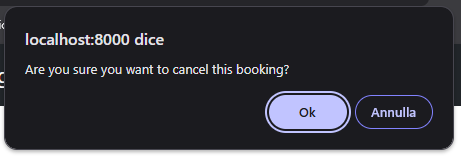
\includegraphics[width=\textwidth, keepaspectratio]{capitoli/immagini/p25.png}
        \par\small\textit{V1 -- stile neutro}
    \end{minipage}
    \hfill
    \begin{minipage}[c]{0.30\textwidth}
        \centering
        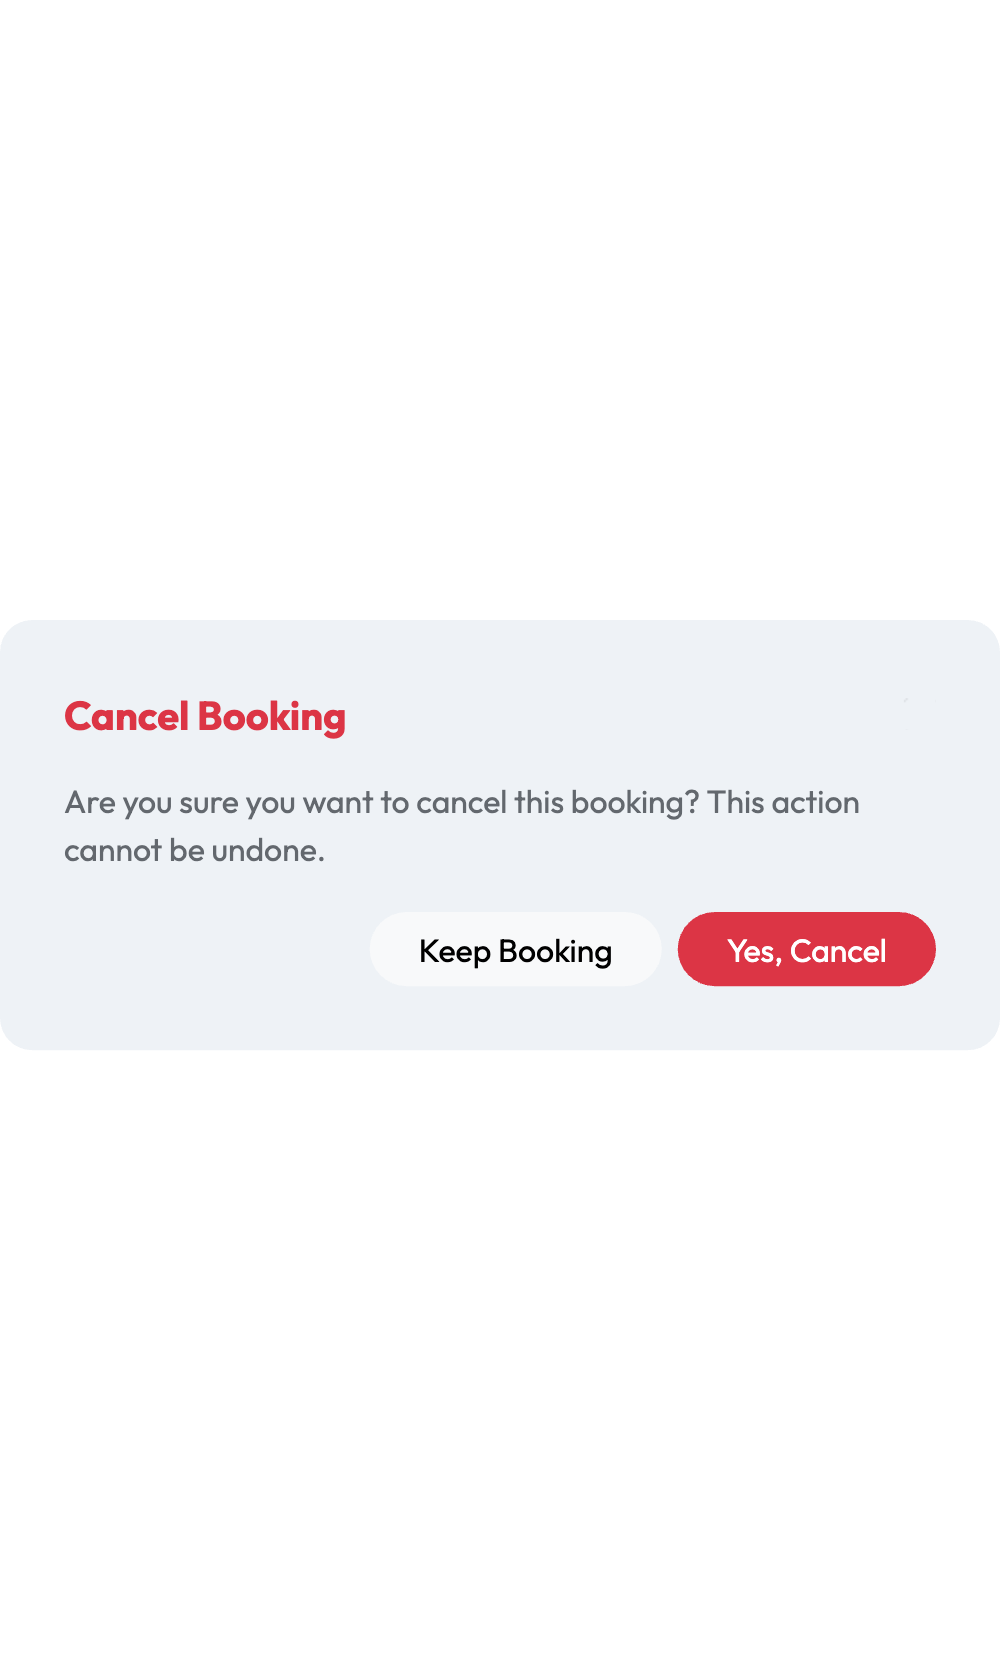
\includegraphics[width=\textwidth, keepaspectratio]{capitoli/immagini/v2/p27_v2.png}
        \par\small\textit{V2 -- \texttt{btn-danger} rosso}
    \end{minipage}
    \caption{P.27 -- Stile bottone: V1 (stile neutro) vs V2 (\texttt{btn-danger} rosso coerente).}
    \label{fig:det_p27}
\end{figure}

\newpage
\subsection{Area Amministratore}

\noindent\textbf{P.28 -- Inconsistenza terminologica} \hfill \textit{Severità: 1}

"Tour", "Visit" e "Booking" erano usati in modo intercambiabile. In V2 la convenzione è: "Tours/Bookings" lato utente finale, "Visits" lato amministrativo.


\noindent\textbf{P.29 -- Incoerenza spaziatura Header} \hfill \textit{Severità: 1}

Le spaziature tra header e contenuto variavano tra le pagine. In V2 la Navbar Bootstrap garantisce padding uniformi in tutta l'applicazione.

\begin{figure}[H]
    \centering
    
\includegraphics[width=0.85\textwidth, keepaspectratio]{capitoli/immagini/p27.png}\\[0.6em]
    
\includegraphics[width=0.85\textwidth, keepaspectratio]{capitoli/immagini/v2/p29_v2.png}
    \caption{P.29 -- Spaziatura header: V1 sopra (padding irregolare) vs V2 sotto (navbar con spaziatura uniforme).}
    \label{fig:det_p29}
\end{figure}

\noindent\textbf{P.30 -- Validazione tardiva aggiunta utente} \hfill \textit{Severità: 2}

Nel modale di creazione utente la validazione avveniva solo al submit. In V2 feedback JavaScript live verifica la password direttamente nel modale amministrativo.

\begin{figure}[H]
    \centering
    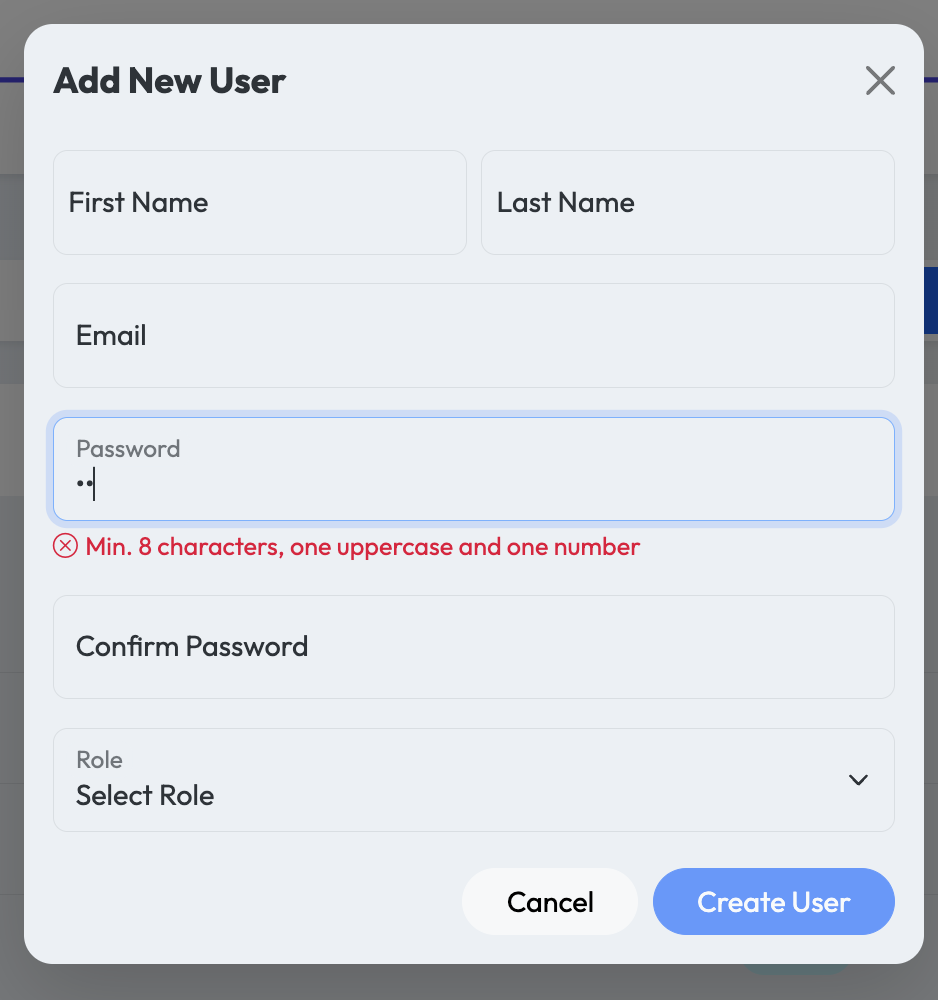
\includegraphics[width=0.40\textwidth, keepaspectratio]{capitoli/immagini/v2/p30_v2.png}
    \caption{P.30 -- Validazione live nel modale admin: indicatori real-time per la password nel configuratore.}
    \label{fig:det_p30}
\end{figure}

\noindent\textbf{P.31 -- Assenza conferma eliminazione} \hfill \textit{Severità: 4}

La criticità più grave del sistema: ogni eliminazione avveniva immediatamente al click. In V2 il Global Delete Confirmation Modal interrompe l'azione e obbliga a una conferma esplicita con avviso "This action cannot be undone".

\begin{figure}[H]
    \centering
    \begin{subfigure}[b]{0.47\textwidth}
        \centering
        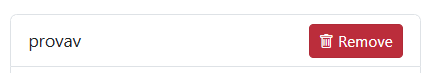
\includegraphics[width=\textwidth, keepaspectratio]{capitoli/immagini/p29.png}
        \caption{V1 (Prima)}
    \end{subfigure}
    \hfill
    \begin{subfigure}[b]{0.47\textwidth}
        \centering
        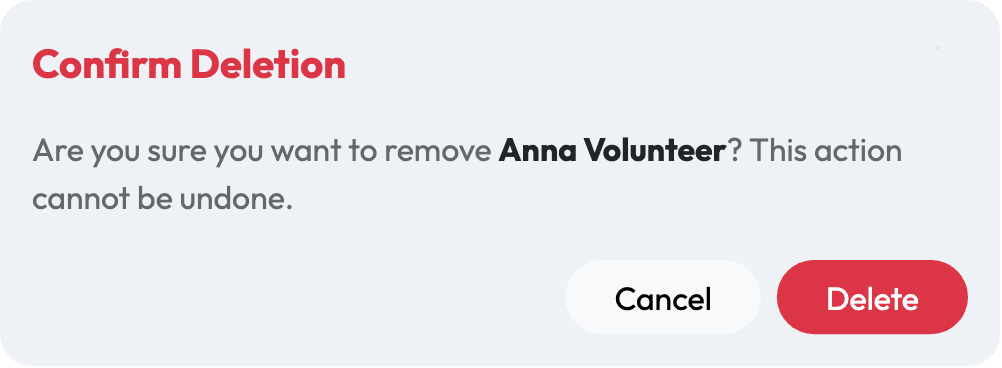
\includegraphics[width=\textwidth, keepaspectratio]{capitoli/immagini/v2/p31_v2.png}
        \caption{V2 (Dopo)}
    \end{subfigure}
    \caption{P.31 -- Conferma eliminazione: V1 (eliminazione immediata) vs V2 (Global Delete Modal).}
    \label{fig:det_p31}
\end{figure}

\noindent\textbf{P.32 -- Disorganizzazione layout Visit Planning} \hfill \textit{Severità: 1}

Il pannello di pianificazione era caotico e difficile da navigare. In V2 le visite sono organizzate in card per mese con intestazioni chiare.

\begin{figure}[H]
    \centering
    \begin{subfigure}[b]{0.47\textwidth}
        \centering
        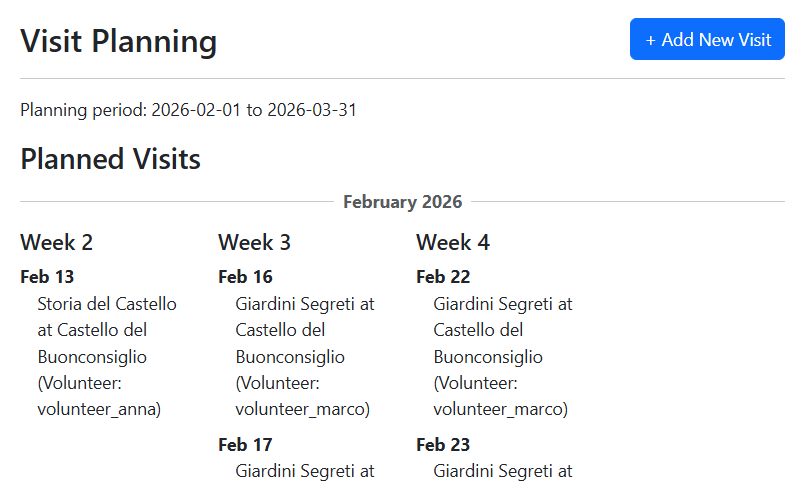
\includegraphics[width=\textwidth, keepaspectratio]{capitoli/immagini/p30.png}
        \caption{V1 (Prima)}
    \end{subfigure}
    \hfill
    \begin{subfigure}[b]{0.47\textwidth}
        \centering
        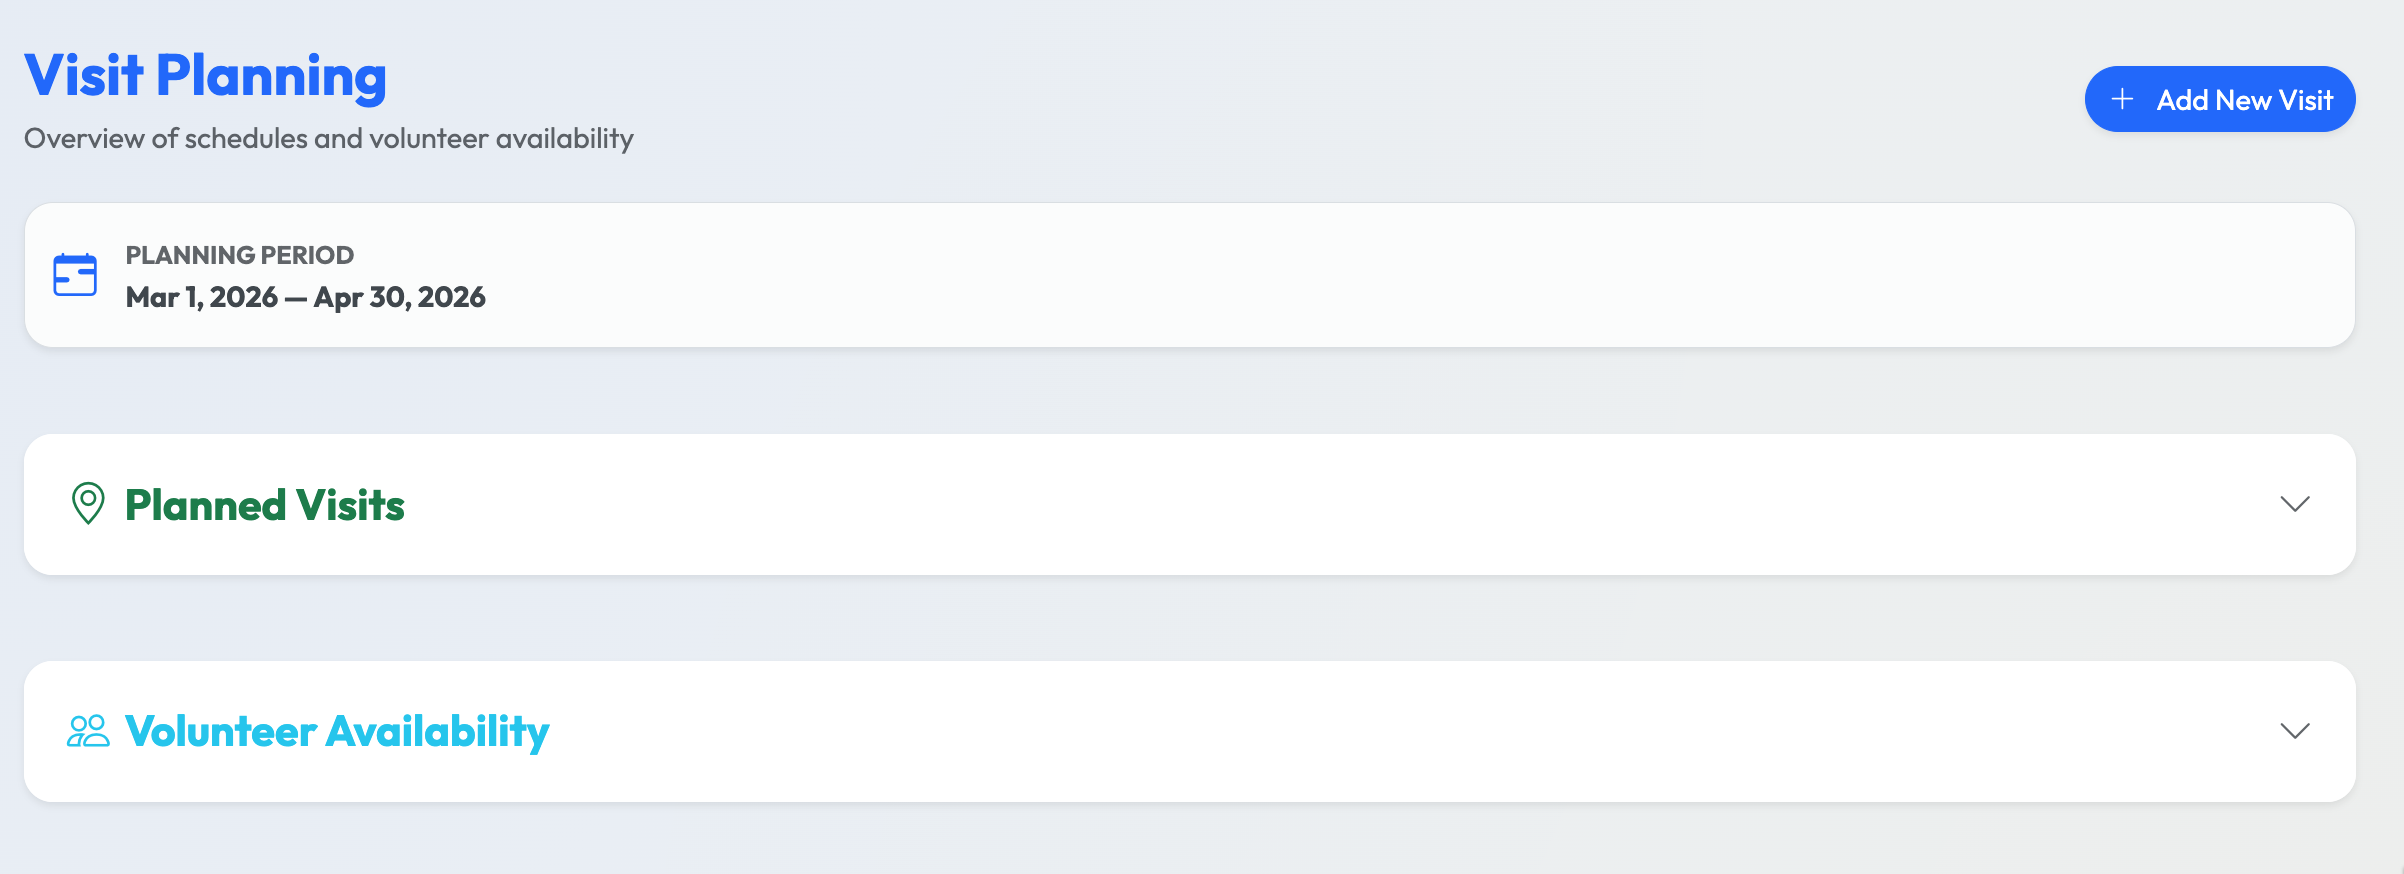
\includegraphics[width=\textwidth, keepaspectratio]{capitoli/immagini/v2/p32_v2.png}
        \caption{V2 (Dopo)}
    \end{subfigure}
    \caption{P.32 -- Visit Planning: V1 (layout disorganizzato) vs V2 (card mensili con sezioni chiare).}
    \label{fig:det_p32}
\end{figure}

\noindent\textbf{P.33 -- Flusso inserimento non intuitivo} \hfill \textit{Severità: 3}

La sequenza di inserimento di una nuova visita non era guidata. In V2 il form presenta un flusso step-by-step: Tipo Visita → Data → Volontario disponibile.

\begin{figure}[H]
    \centering
    \begin{subfigure}[b]{0.47\textwidth}
        \centering
        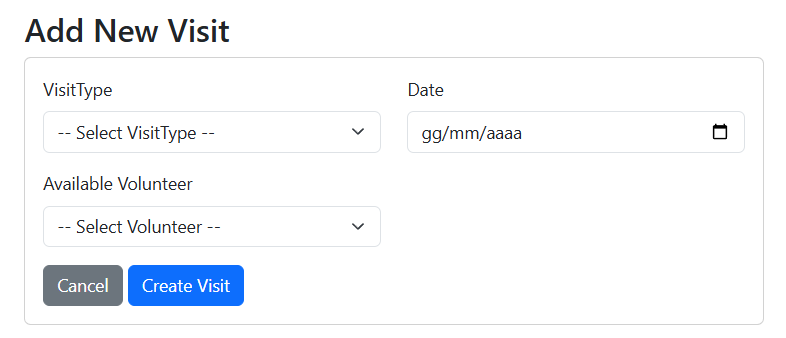
\includegraphics[width=\textwidth, keepaspectratio]{capitoli/immagini/p31.png}
        \caption{V1 (Prima)}
    \end{subfigure}
    \hfill
    \begin{subfigure}[b]{0.47\textwidth}
        \centering
        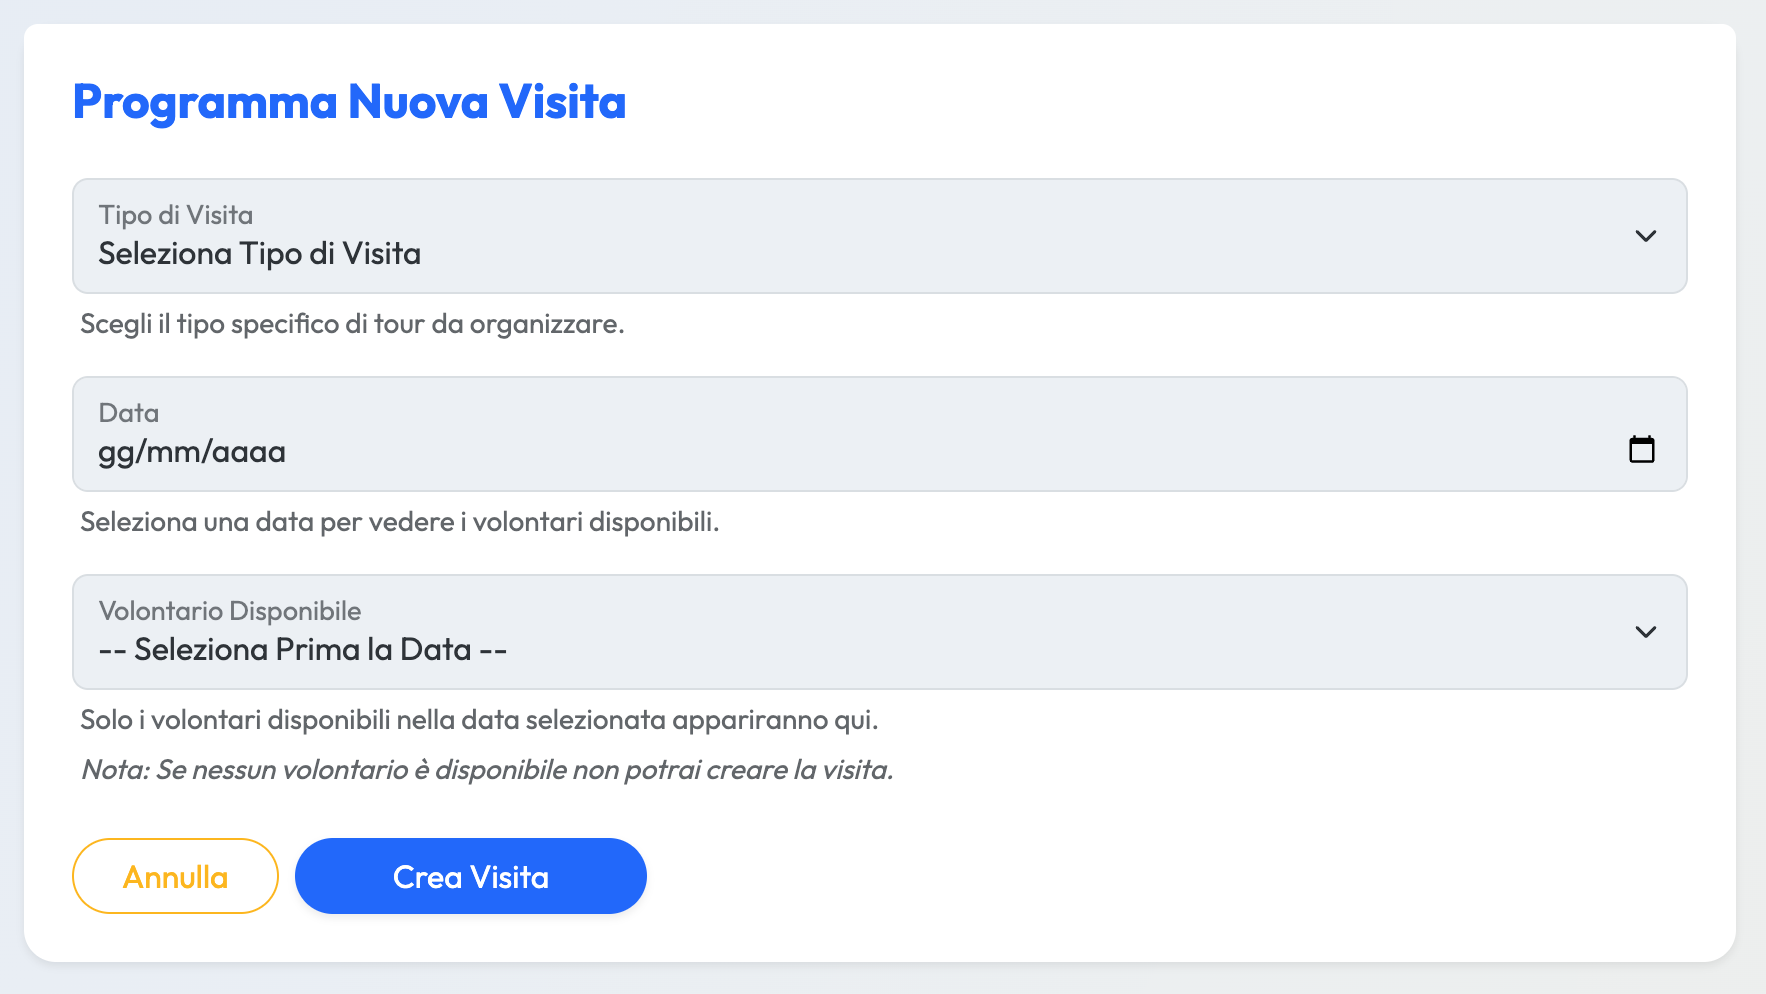
\includegraphics[width=\textwidth, keepaspectratio]{capitoli/immagini/v2/p33_v2.png}
        \caption{V2 (Dopo)}
    \end{subfigure}
    \caption{P.33 -- Add Visit: V1 (form non guidato) vs V2 (flusso Tipo → Data → Volontario).}
    \label{fig:det_p33}
\end{figure}

\noindent\textbf{P.34 -- Mancanza feedback su vincoli} \hfill \textit{Severità: 3}

L'utente non riceveva indicazioni sui vincoli procedurali prima del submit. In V2 help text contestuali appaiono accanto ai campi critici (data minima, assenza volontari disponibili).

\begin{figure}[H]
    \centering
    \begin{subfigure}[b]{0.47\textwidth}
        \centering
        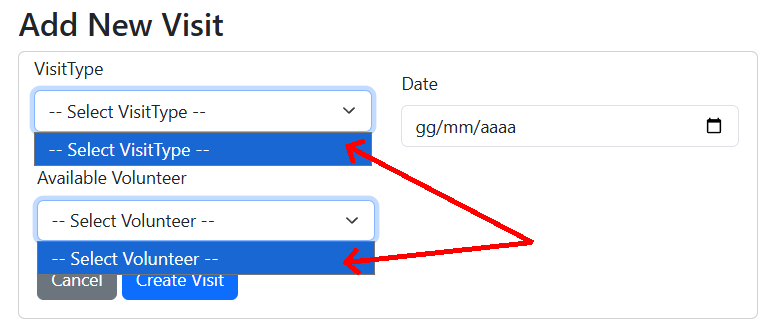
\includegraphics[width=\textwidth, keepaspectratio]{capitoli/immagini/p32.png}
        \caption{V1 (Prima)}
    \end{subfigure}
    \hfill
    \begin{subfigure}[b]{0.47\textwidth}
        \centering
        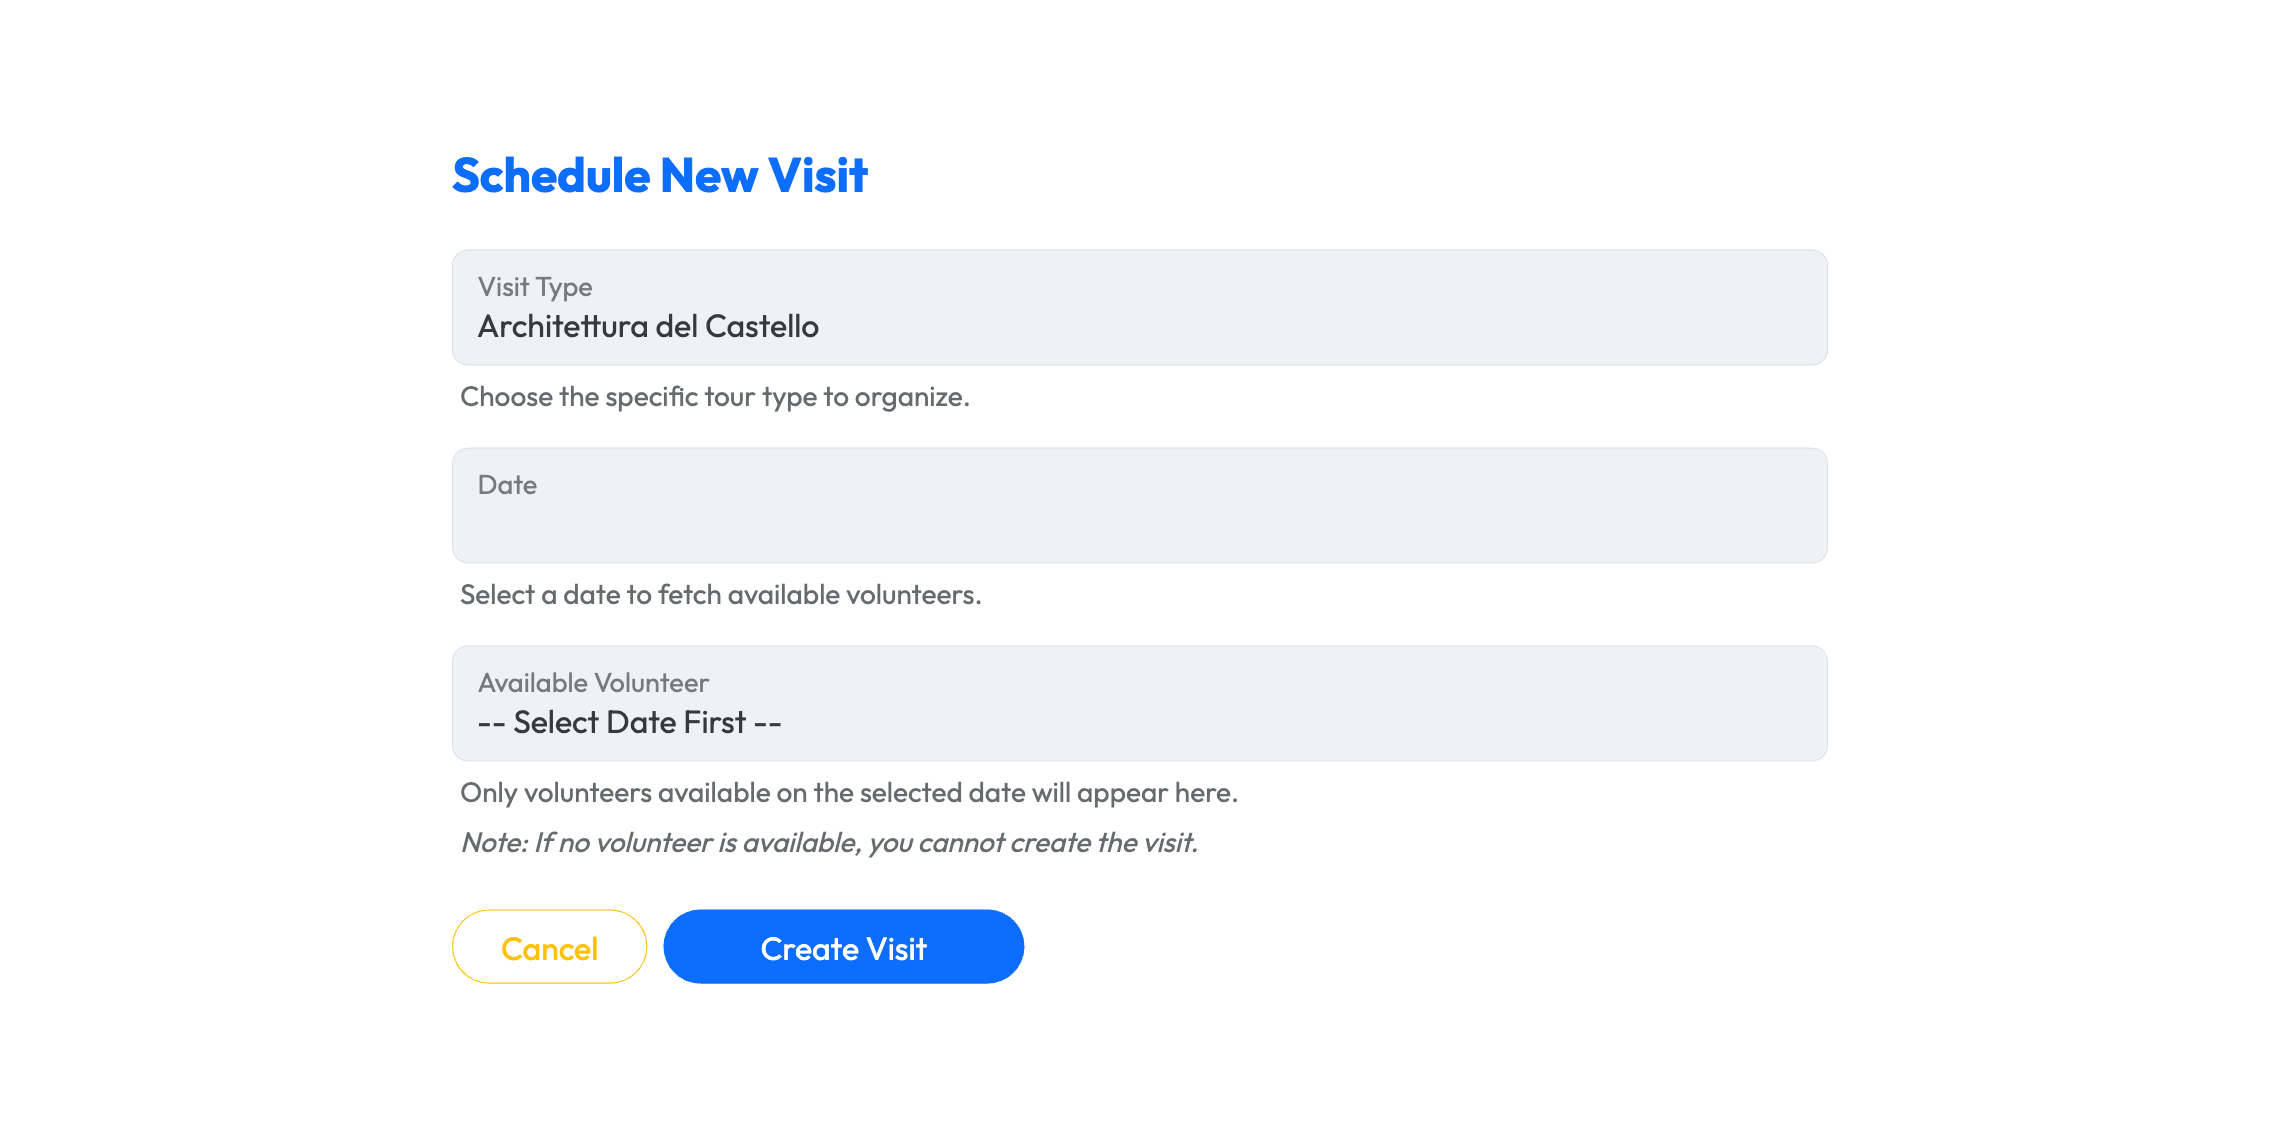
\includegraphics[width=\textwidth, keepaspectratio]{capitoli/immagini/v2/p34_v2.png}
        \caption{V2 (Dopo)}
    \end{subfigure}
    \caption{P.34 -- Feedback vincoli: V1 (nessun help text) vs V2 (indicazioni contestuali accanto ai campi).}
    \label{fig:det_p34}
\end{figure}

\noindent\textbf{P.40 -- Colore bottone non coerente} \hfill \textit{Severità: 2}

Il bottone "Change Password" nella pagina profilo usava il rosso, colore semanticamente associato al pericolo. In V2 è allineato al Design System con uno stile neutro.

\begin{figure}[H]
    \centering
    \begin{subfigure}[b]{0.47\textwidth}
        \centering
        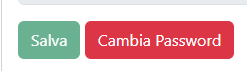
\includegraphics[width=\textwidth, keepaspectratio]{capitoli/immagini/p34.png}
        \caption{V1 (Prima)}
    \end{subfigure}
    \hfill
    \begin{subfigure}[b]{0.47\textwidth}
        \centering
        
\includegraphics[width=\textwidth, keepaspectratio]{capitoli/immagini/v2/p40_v2.png}
        \caption{V2 (Dopo)}
    \end{subfigure}
    \caption{P.40 -- Bottone profilo: V1 (rosso fuorviante) vs V2 (stile neutro coerente).}
    \label{fig:det_p40}
\end{figure}

\newpage
\subsection{Area Volontario (Guida)}

\noindent\textbf{P.37 -- Assenza indicazioni operative} \hfill \textit{Severità: 2}

Le guide non disponevano di promemoria operativi nella pagina delle visite assegnate. In V2 un banner \texttt{alert-info} fornisce istruzioni specifiche: puntualità, verifica booking code, gestione biglietti e contatto organizzativo in caso di imprevisti.

\begin{figure}[H]
    \centering
    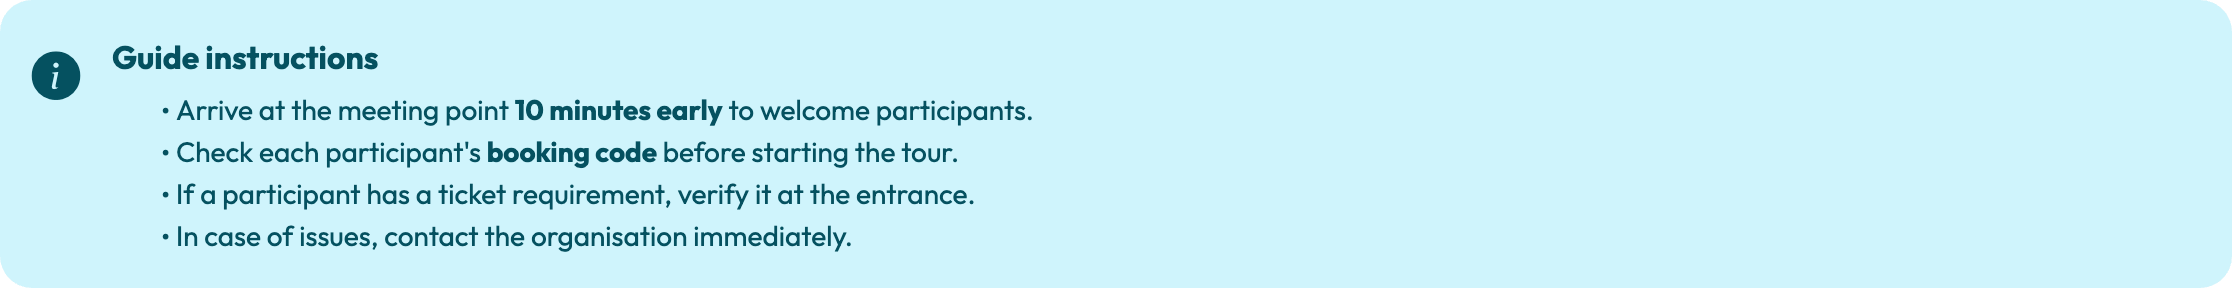
\includegraphics[width=0.85\textwidth, keepaspectratio]{capitoli/immagini/v2/p37_v2.png}
    \caption{P.37 -- Banner istruzioni: V2 con promemoria operativo nella pagina "My Assigned Visits".}
    \label{fig:det_p37}
\end{figure}

\noindent\textbf{P.38 -- Ridondanza nome volontario nelle card} \hfill \textit{Severità: 1}

Il nome del volontario assegnato compariva sempre, anche nella vista privata della guida stessa. In V2 il nome è nascosto se coincide con l'utente loggato, visibile solo ad altri ruoli.

\begin{figure}[H]
    \centering
    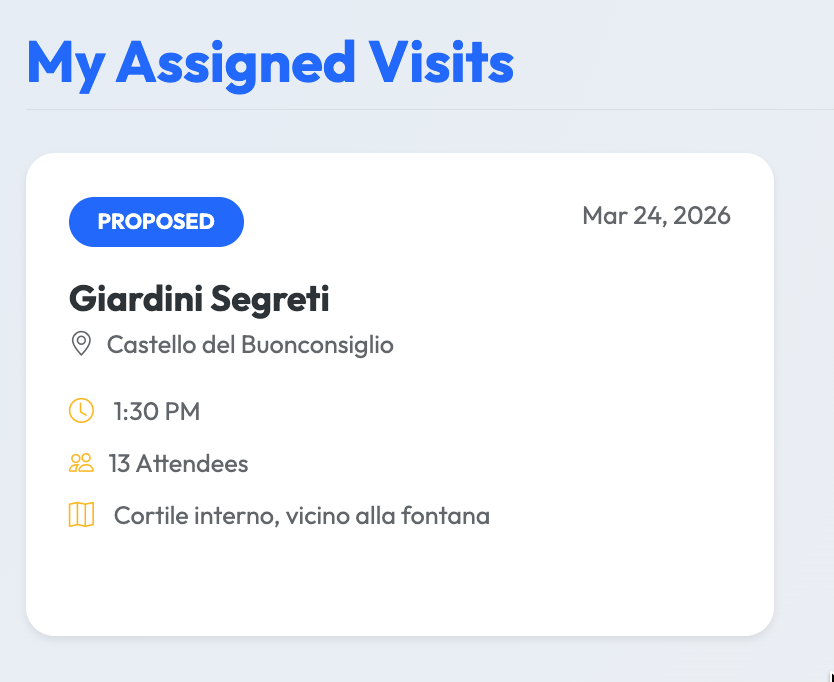
\includegraphics[width=0.55\textwidth, keepaspectratio]{capitoli/immagini/v2/p38_v2.png}
    \caption{P.38 -- Ridondanza nome: V2 -- il nome del volontario è nascosto quando coincide con l'utente corrente.}
    \label{fig:det_p38}
\end{figure}

% ─────────────────────────────────────────────────────────────────────────────
\section{Problemi Non Risolti}
\label{sec:problemi_aperti}

Cinque problemi identificati nel Capitolo 3 non sono stati risolti nella presente versione del sistema. In tutti i casi la decisione è motivata da complessità implementativa, vincoli di scope del progetto o dalla bassa severità rapportata all'impatto atteso sull'esperienza d'uso. Tali problemi restano candidati prioritari per iterazioni future.

\begin{table}[H]
\centering
\renewcommand{\arraystretch}{1.5}
\small
\begin{tabularx}{\textwidth}{|c|X|c|X|}
\hline
\textbf{P\#} & \textbf{Problema} & \textbf{Sev.} & \textbf{Motivazione della mancata risoluzione} \\ \hline
1  & Cursore non coerente su elementi cliccabili & 2 & Richiede un audit sistematico di tutti gli elementi interattivi dell'interfaccia con aggiunta di \texttt{cursor: pointer} nei CSS globali. Il rischio di regressioni stilistiche ha portato a posticipare l'intervento. \\ \hline
2  & Assenza notifica rischio annullamento visita & 3 & Necessita di logica server-side per confrontare partecipanti iscritti e soglia minima, con generazione di alert contestuali nella dashboard. Fuori dallo scope della riprogettazione corrente. \\ \hline
36 & Mancanza selezione multipla nel calendario  & 2 & Richiederebbe un refactoring significativo del componente JavaScript del calendario disponibilità (shortcut "Tutti i weekend" / "Tutto il mese"). Identificato come miglioramento futuro ad alta priorità. \\ \hline
39 & Messaggio stato vuoto senza Call to Action  & 2 & La funzionalità principale rimane intatta; la CTA verso la Homepage sarà integrata in un rilascio successivo a basso rischio. \\ \hline
—  & Scroll inaspettato al cambio pagina         & — & Comportamento collaterale del pattern "Load More" asincrono: la chiamata a \texttt{scrollIntoView()} si comporta diversamente a seconda del browser. Richiede refactoring della logica di scroll nel componente Alpine.js. \\ \hline
\end{tabularx}
\caption{Problemi identificati nel Capitolo 3 non risolti nella versione corrente.}
\label{tab:problemi_aperti}
\end{table}

\chapter{Esperimento con gli utenti}
\label{ch:esperimento}

Una volta conclusa la riprogettazione del sito sono stati eseguiti degli esperimenti con gli utenti: lo scopo di questa fase è stato quello di raccogliere dati relativi all'utilizzo del sistema da parte di utenti reali per poi usarli, nel capitolo successivo, per analizzare nel dettaglio gli effettivi miglioramenti apportati.
Il test ha confrontato le due versioni del sistema --- V1 (originale) e V2 (riprogettata) --- su un campione temporale di partecipanti. In questo capitolo verranno illustrate le modalità con cui sono stati svolti questi esperimenti.

\section{Caratteristiche dell'esperimento}

Per gli esperimenti di usabilità è stato scelto l'approccio "within-subject", che implica che ogni gruppo di utenti abbia testato entrambe le condizioni sperimentali, ossia le due versioni del sito, in ordine variabile: questa metodologia è preferibile in contesti nei quali sono ridotti i problemi di apprendimento, richiede meno utenti e comporta minori problemi legati alla variabilità degli stessi.

È stata inoltre utilizzata la metodologia di \textit{counterbalancing} per evitare problemi legati all'apprendimento degli utenti da una versione all'altra. Un totale di 10 utenti è stato selezionato e diviso in due gruppi distinti:
\begin{itemize}
    \item \textbf{Gruppo A}: ha sperimentato inizialmente la "Versione 1" del sito (originale) seguita dalla "Versione 2" (riprogettata).
    \item \textbf{Gruppo B}: ha sperimentato inizialmente la "Versione 2" del sito seguita dalla "Versione 1".
\end{itemize}

Si è cercato, per quanto possibile, di garantire omogeneità e bilanciamento tra i gruppi considerando le informazioni demografiche raccolte attraverso questionari preliminari (Sesso, Età, Titolo di studio, Conoscenze informatiche).

\section{Ambiente}

Per simulare il contesto di utilizzo reale del sistema, si è deciso di eseguire gli esperimenti in luoghi familiari agli utenti (come aule studio e abitazioni private), in modo da metterli a loro agio.
Tutti gli esperimenti sono stati eseguiti su un computer portatile fornito dallo sperimentatore (con browser Chrome), in modo da ricreare la stessa situazione e ambiente applicativo (Laravel locale) per tutti i soggetti.
Lo sperimentatore si trovava nella stessa stanza in posizione non intrusiva, intervenendo esclusivamente su esplicita richiesta del partecipante.

\section{Dati raccolti}

I dati raccolti dallo sperimentatore sono sia quantitativi che qualitativi, così da permettere sia analisi statistiche che valutazioni di natura descrittiva.
Per ogni compito sono stati raccolti i seguenti dati quantitativi:
\begin{itemize}
    \item \textbf{Completamento} (indica se il task è stato completato, completato con aiuto, o non completato);
    \item \textbf{Tempo impiegato} per il completamento del compito;
    \item \textbf{Numero di click} necessari al completamento;
    \item \textbf{Numero di errori} eseguiti durante la navigazione.
\end{itemize}

Per i dati qualitativi si hanno:
\begin{itemize}
    \item \textbf{Note sperimentatore};
    \item \textbf{Commenti dell'utente} (\textit{Think Aloud}).
\end{itemize}

Inoltre ogni utente ha valutato la \textbf{difficoltà} di ogni scenario su una scala appropriata e ha compilato il questionario \textbf{SUS (System Usability Scale)} per il grado di usabilità, affiancato dall'indice \textbf{NPS (Net Promoter Score)}.

\section{Scelta degli sperimentatori}

Per l'esecuzione degli esperimenti si è scelto di impiegare un solo sperimentatore, responsabile dell'osservazione e dell'annotazione delle metriche, con funzione anche di facilitatore per mettere a proprio agio gli utenti in caso di stallo prolungato. Lo sperimentatore è rimasto invariato per tutti i test svolti.

\section{Scelta degli utenti}

Trattandosi di un sito destinato ad un'ampia varietà di persone (dai fruitori occasionali di visite guidate ai volontari), sono stati scelti 10 utenti eterogenei: 5 per il Gruppo A e 5 per il Gruppo B. 
Prima dell'inizio della sessione, ciascun partecipante ha compilato il \textbf{questionario anagrafico} (oltre ad aver accettato le clausole del consenso informato GDPR). 

La tabella seguente riassume la suddivisione:

\begin{table}[H]
\centering
\renewcommand{\arraystretch}{1.4}
\small
\begin{tabular}{|c|c|c|c|c|c|c|}
\hline
\textbf{ID} & \textbf{Età} & \textbf{Genere} & \textbf{Titolo di studio} & \textbf{Competenza informatica} & \textbf{Gruppo (Ordine)} \\
\hline
U01 & 22 & M & Laurea      & Alta  & Gruppo A (V1 $\to$ V2) \\ \hline
U02 & 20 & F & Diploma     & Media & Gruppo A (V1 $\to$ V2) \\ \hline
U03 & 38 & M & Laurea      & Alta  & Gruppo A (V1 $\to$ V2) \\ \hline
U04 & 26 & F & Laurea      & Media & Gruppo A (V1 $\to$ V2) \\ \hline
U05 & 54 & M & Diploma     & Bassa & Gruppo A (V1 $\to$ V2) \\ \hline
U06 & 23 & F & Laurea      & Alta  & Gruppo B (V2 $\to$ V1) \\ \hline
U07 & 28 & M & Laurea      & Media & Gruppo B (V2 $\to$ V1) \\ \hline
U08 & 45 & F & Laurea      & Media & Gruppo B (V2 $\to$ V1) \\ \hline
U09 & 33 & M & Diploma     & Bassa & Gruppo B (V2 $\to$ V1) \\ \hline
U10 & 21 & F & Laurea      & Alta  & Gruppo B (V2 $\to$ V1) \\ \hline
\end{tabular}
\caption{Panoramica anagrafica dei partecipanti al test di usabilità ($n=10$).}
\label{tab:partecipanti}
\end{table}

Maggiori dettagli demografici e relative distribuzioni grafiche saranno illustrati approfonditamente nel capitolo dell'analisi dei risultati (Capitolo 6).

\section{Scelta dei compiti e Moduli}

L'esperimento è basato su \textbf{11 compiti} (task) pensati per coprire il ciclo di vita completo della piattaforma: dalla ricerca di informazioni base, alla registrazione, per poi valutare le funzionalità transazionali (prenotazioni) e le interfacce riservate ai ruoli di volontario e amministratore. 
Per standardizzare lo svolgimento, oltre al questionario anagrafico iniziale, è stato predisposto un \textbf{modulo strutturato} (riportato di seguito) compilato fisicamente dallo sperimentatore per annotare click, tempi, errori e i commenti \textit{Think Aloud} degli utenti in tempo reale.

\vspace{0.5cm}

% T1
\noindent
\framebox[\linewidth]{
\begin{minipage}{0.96\linewidth}
\vspace{0.2cm}
\textbf{T1. Dire dove si trova la sede dell'organizzazione} \\[0.15cm]
\textit{Risposta attesa:} Via Branze 38, Brescia \\
\textbf{Tempo limite:} 1 min \\[0.2cm]
\hrule \vspace{0.2cm}
Tempo impiegato: \rule{2.5cm}{0.4pt} \hfill Click: \rule{2cm}{0.4pt} \hfill Errori: \rule{2cm}{0.4pt} \\[0.2cm]
Completato: \quad [\quad] Sì \qquad [\quad] No \qquad [\quad] Con Aiuto \\[0.2cm]
\hrule \vspace{0.2cm}
\textbf{Note Sperimentatore:} \\[1.2cm]
\textbf{Commenti Utente:} \\[1.2cm]
\end{minipage}} \vspace{0.5cm}

% T2
\noindent
\framebox[\linewidth]{
\begin{minipage}{0.96\linewidth}
\vspace{0.2cm}
\textbf{T2. Registrati come nuovo utente e accedi} \\[0.15cm]
\textit{Azione attesa:} Log-in completato con successo. \\
\textbf{Tempo limite:} 2 min \\[0.2cm]
\hrule \vspace{0.2cm}
Tempo impiegato: \rule{2.5cm}{0.4pt} \hfill Click: \rule{2cm}{0.4pt} \hfill Errori: \rule{2cm}{0.4pt} \\[0.2cm]
Completato: \quad [\quad] Sì \qquad [\quad] No \qquad [\quad] Con Aiuto \\[0.2cm]
\hrule \vspace{0.2cm}
\textbf{Note Sperimentatore:} \\[1.2cm]
\textbf{Commenti Utente:} \\[1.2cm]
\end{minipage}} \vspace{0.5cm}

% T3
\noindent
\framebox[\linewidth]{
\begin{minipage}{0.96\linewidth}
\vspace{0.2cm}
\textbf{T3. Prenota una visita guidata a "Castello di Sera" del X (seconda riga) per 2 persone} \\[0.15cm]
\textit{Azione attesa:} Prenotazione generata nel profilo. \\
\textbf{Tempo limite:} 2 min \\[0.2cm]
\hrule \vspace{0.2cm}
Tempo impiegato: \rule{2.5cm}{0.4pt} \hfill Click: \rule{2cm}{0.4pt} \hfill Errori: \rule{2cm}{0.4pt} \\[0.2cm]
Completato: \quad [\quad] Sì \qquad [\quad] No \qquad [\quad] Con Aiuto \\[0.2cm]
\hrule \vspace{0.2cm}
\textbf{Note Sperimentatore:} \\[1.2cm]
\textbf{Commenti Utente:} \\[1.2cm]
\end{minipage}} \vspace{0.5cm}

% T4
\noindent
\framebox[\linewidth]{
\begin{minipage}{0.96\linewidth}
\vspace{0.2cm}
\textbf{T4. Trova il codice della prenotazione appena effettuata} \\[0.15cm]
\textit{Risposta attesa:} Dettatura del token univoco generato randomicamente dal sistema. \\
\textbf{Tempo limite:} 2 min \\[0.2cm]
\hrule \vspace{0.2cm}
Tempo impiegato: \rule{2.5cm}{0.4pt} \hfill Click: \rule{2cm}{0.4pt} \hfill Errori: \rule{2cm}{0.4pt} \\[0.2cm]
Completato: \quad [\quad] Sì \qquad [\quad] No \qquad [\quad] Con Aiuto \\[0.2cm]
\hrule \vspace{0.2cm}
\textbf{Note Sperimentatore:} \\[1.2cm]
\textbf{Commenti Utente:} \\[1.2cm]
\end{minipage}} \vspace{0.5cm}

% T5
\noindent
\framebox[\linewidth]{
\begin{minipage}{0.96\linewidth}
\vspace{0.2cm}
\textbf{T5. Cancella la prenotazione appena effettuata} \\[0.15cm]
\textit{Azione attesa:} Modale di conferma d'annullamento superato. \\
\textbf{Tempo limite:} 1 min \\[0.2cm]
\hrule \vspace{0.2cm}
Tempo impiegato: \rule{2.5cm}{0.4pt} \hfill Click: \rule{2cm}{0.4pt} \hfill Errori: \rule{2cm}{0.4pt} \\[0.2cm]
Completato: \quad [\quad] Sì \qquad [\quad] No \qquad [\quad] Con Aiuto \\[0.2cm]
\hrule \vspace{0.2cm}
\textbf{Note Sperimentatore:} \\[1.2cm]
\textbf{Commenti Utente:} \\[1.2cm]
\end{minipage}} \vspace{0.5cm}

% T6
\noindent
\framebox[\linewidth]{
\begin{minipage}{0.96\linewidth}
\vspace{0.2cm}
\textbf{T6. Effettua il logout dall'utente attuale ed esegui il login come volontario (anna@example.com)} \\[0.15cm]
\textit{Azione attesa:} Switch dell'account superato con password: password123. \\
\textbf{Tempo limite:} 1 min \\[0.2cm]
\hrule \vspace{0.2cm}
Tempo impiegato: \rule{2.5cm}{0.4pt} \hfill Click: \rule{2cm}{0.4pt} \hfill Errori: \rule{2cm}{0.4pt} \\[0.2cm]
Completato: \quad [\quad] Sì \qquad [\quad] No \qquad [\quad] Con Aiuto \\[0.2cm]
\hrule \vspace{0.2cm}
\textbf{Note Sperimentatore:} \\[1.2cm]
\textbf{Commenti Utente:} \\[1.2cm]
\end{minipage}} \vspace{0.5cm}

% T7
\noindent
\framebox[\linewidth]{
\begin{minipage}{0.96\linewidth}
\vspace{0.2cm}
\textbf{T7. Imposta la disponibilità a un giorno qualsiasi non già impostato (es 25/04/26)} \\[0.15cm]
\textit{Azione attesa:} Slot sul calendario personale indicato come disp. \\
\textbf{Tempo limite:} 1 min \\[0.2cm]
\hrule \vspace{0.2cm}
Tempo impiegato: \rule{2.5cm}{0.4pt} \hfill Click: \rule{2cm}{0.4pt} \hfill Errori: \rule{2cm}{0.4pt} \\[0.2cm]
Completato: \quad [\quad] Sì \qquad [\quad] No \qquad [\quad] Con Aiuto \\[0.2cm]
\hrule \vspace{0.2cm}
\textbf{Note Sperimentatore:} \\[1.2cm]
\textbf{Commenti Utente:} \\[1.2cm]
\end{minipage}} \vspace{0.5cm}

% T8
\noindent
\framebox[\linewidth]{
\begin{minipage}{0.96\linewidth}
\vspace{0.2cm}
\textbf{T8. Effettua il logout ed esegui il login come amministratore (admin@example.com)} \\[0.15cm]
\textit{Azione attesa:} Dashboard admin raggiunta con successo (password123). \\
\textbf{Tempo limite:} 30 s \\[0.2cm]
\hrule \vspace{0.2cm}
Tempo impiegato: \rule{2.5cm}{0.4pt} \hfill Click: \rule{2cm}{0.4pt} \hfill Errori: \rule{2cm}{0.4pt} \\[0.2cm]
Completato: \quad [\quad] Sì \qquad [\quad] No \qquad [\quad] Con Aiuto \\[0.2cm]
\hrule \vspace{0.2cm}
\textbf{Note Sperimentatore:} \\[1.2cm]
\textbf{Commenti Utente:} \\[1.2cm]
\end{minipage}} \vspace{0.5cm}

% T9
\noindent
\framebox[\linewidth]{
\begin{minipage}{0.96\linewidth}
\vspace{0.2cm}
\textbf{T9. Crea una visita per la data impostata come disponibile da volontario prima (es. 25/04/26)} \\[0.15cm]
\textit{Azione attesa:} Creare l'evento associando la guida "Anna". \\
\textbf{Tempo limite:} 2 min \\[0.2cm]
\hrule \vspace{0.2cm}
Tempo impiegato: \rule{2.5cm}{0.4pt} \hfill Click: \rule{2cm}{0.4pt} \hfill Errori: \rule{2cm}{0.4pt} \\[0.2cm]
Completato: \quad [\quad] Sì \qquad [\quad] No \qquad [\quad] Con Aiuto \\[0.2cm]
\hrule \vspace{0.2cm}
\textbf{Note Sperimentatore:} \\[1.2cm]
\textbf{Commenti Utente:} \\[1.2cm]
\end{minipage}} \vspace{0.5cm}

% T10
\noindent
\framebox[\linewidth]{
\begin{minipage}{0.96\linewidth}
\vspace{0.2cm}
\textbf{T10. Elimina una visita da un luogo qualsiasi} \\[0.15cm]
\textit{Azione attesa:} Eliminazione riuscita e rimozione dall'elenco. \\
\textbf{Tempo limite:} 2 min \\[0.2cm]
\hrule \vspace{0.2cm}
Tempo impiegato: \rule{2.5cm}{0.4pt} \hfill Click: \rule{2cm}{0.4pt} \hfill Errori: \rule{2cm}{0.4pt} \\[0.2cm]
Completato: \quad [\quad] Sì \qquad [\quad] No \qquad [\quad] Con Aiuto \\[0.2cm]
\hrule \vspace{0.2cm}
\textbf{Note Sperimentatore:} \\[1.2cm]
\textbf{Commenti Utente:} \\[1.2cm]
\end{minipage}} \vspace{0.5cm}

% T11
\noindent
\framebox[\linewidth]{
\begin{minipage}{0.96\linewidth}
\vspace{0.2cm}
\textbf{T11. Cambia password da password123 a Admin123} \\[0.15cm]
\textit{Azione attesa:} Raggiungere le impostazioni del profilo Admin e mutare le credenziali. \\
\textbf{Tempo limite:} 1 min \\[0.2cm]
\hrule \vspace{0.2cm}
Tempo impiegato: \rule{2.5cm}{0.4pt} \hfill Click: \rule{2cm}{0.4pt} \hfill Errori: \rule{2cm}{0.4pt} \\[0.2cm]
Completato: \quad [\quad] Sì \qquad [\quad] No \qquad [\quad] Con Aiuto \\[0.2cm]
\hrule \vspace{0.2cm}
\textbf{Note Sperimentatore:} \\[1.2cm]
\textbf{Commenti Utente:} \\[1.2cm]
\end{minipage}} \vspace{0.5cm}

\chapter{Analisi dei risultati}
\label{ch:analisi}

In questa sezione viene fornita un'analisi dei dati derivati dagli esperimenti condotti con gli utenti. Tale analisi si articola in tre macro-aree: i profili demografici estratti dal questionario iniziale, l'analisi puntuale compito per compito, e i risultati dei questionari finali (SUS e NPS) corredati dai commenti qualitativi.

\section{Profili demografici sperimentatori}

Un totale di 12 utenti è stato selezionato e diviso in due gruppi (A e B), ciascuno composto da 6 partecipanti. Di seguito vengono riportati i risultati ottenuti dall'analisi anagrafica, necessaria per garantire che i campioni fossero bilanciati e rappresentativi. Non essendovi sbilanciamenti severi si è assunto che i gruppi fossero idonei all'esperimento \textit{within-subject}.

\subsection{Genere}
Il campione è composto da 6 uomini e 6 donne, perfettamente bilanciato. Nel Gruppo A la distribuzione è di 3 uomini (U01, U05, U06) e 3 donne (U02, U03, U04); nel Gruppo B si hanno parimenti 3 uomini (U07, U09, U12) e 3 donne (U08, U10, U11). La distribuzione è del tutto equa tra i gruppi.

\subsection{Età}
L'età dei partecipanti spazia dai 19 ai 57 anni, con due cluster demografici netti e intenzionali:
\begin{itemize}
    \item \textbf{Cluster giovani} (19--22 anni): U04, U05, U06, U10, U11, U12 — alta familiarità tecnologica, esperienza con prenotazioni online.
    \item \textbf{Cluster maturi} (51--57 anni): U01, U02, U03, U07, U08, U09 — competenze informatiche più limitate, minore abitudine alle prenotazioni digitali.
\end{itemize}
Questa bipartizione è stata deliberata per testare l'accessibilità trasversale della piattaforma, verificando se V2 risulta migliorata sia per utenti esperti che per utenti meno avvezzi alla tecnologia.

\subsection{Titolo di studio e Competenze Informatiche}
Il campione presenta una distribuzione variegata: 3 partecipanti con Laurea Triennale (U04, U10, U12), 5 con Diploma (U03, U05, U06, U08, U11) e 4 con Licenza Media (U01, U02, U07, U09). Le competenze informatiche autovalutate su scala 1--5 riflettono fedelmente la bipartizione anagrafica: il cluster giovane si attesta su valori 3--5 (Media/Alta), mentre il cluster maturo registra valori 1--2 (Bassa). Entrambi i gruppi A e B includono una rappresentanza bilanciata di utenti ad alta e bassa competenza.

\subsection{Autonomia nelle prenotazioni online}
Il questionario anagrafico includeva una domanda sull'autonomia nell'effettuare prenotazioni online (scala 0--2: mai / a volte / sempre). Il dato è particolarmente rilevante per una piattaforma di prenotazione visite: 7 partecipanti su 12 dichiarano piena autonomia (valore 2), 4 autonomia parziale (valore 1) e 1 partecipante (U01) non ha mai effettuato prenotazioni online in autonomia. Questo garantisce la presenza di utenti "nuovi" al paradigma di prenotazione digitale, rendendo il test più significativo.

\subsection{Daltonismo}
Nessun partecipante ha dichiarato di soffrire di daltonismo, tuttavia, a livello precauzionale e di standard di accessibilità, l'interfaccia V2 mantiene un rapporto di contrasto a norma WCAG e affida i feedback visivi non solo al colore ma anche a etichette esplicite (es. Status Badge azzurro per "Upcoming", grigio per "Complete").

\section{Analisi dei compiti}

In questa sezione viene esposta l'analisi dei dati raccolti. Per ciascun compito (da 1 a 11) i dati quantitativi sono stati elaborati confrontando le metriche ottenute nella Versione 1 (originale) e nella Versione 2 (riprogettata). Indichiamo con "C" i compiti completati in autonomia, "CA" per completati con aiuto e "NC" per non completati.

\subsection{Compito 1: Sede organizzazione}
\begin{table}[H]
\centering
\renewcommand{\arraystretch}{1.2}
\small
\begin{tabular}{|l|c|c|}
\hline
\textbf{Metrica} & \textbf{Versione 1} & \textbf{Versione 2} \\
\hline
Completato & 8 (C), 1 (CA), 1 (NC) & 10 (C), 0 (CA), 0 (NC) \\ \hline
Tempo Medio & 75 s & 22 s \\ \hline
Click Medi & 6 & 2 \\ \hline
Errori Medi & 1.2 & 0.1 \\ \hline
Difficoltà Percepita & Facile & Molto facile \\ \hline
\end{tabular}
\end{table}
\textbf{Commenti:} Nella V1, l'indirizzo era nascosto all'interno di sottomenu testuali; nella V2 è immediatamente visibile nel footer universale. Tempi di completamento abbattuti di oltre il 60\%.

\subsection{Compito 2: Registrazione e accesso}
\begin{table}[H]
\centering
\renewcommand{\arraystretch}{1.2}
\small
\begin{tabular}{|l|c|c|}
\hline
\textbf{Metrica} & \textbf{Versione 1} & \textbf{Versione 2} \\
\hline
Completato & 7 (C), 2 (CA), 1 (NC) & 10 (C), 0 (CA), 0 (NC) \\ \hline
Tempo Medio & 148 s & 92 s \\ \hline
Click Medi & 13 & 8 \\ \hline
Errori Medi & 1.9 & 0.3 \\ \hline
Difficoltà Percepita & Media & Facile \\ \hline
\end{tabular}
\end{table}
\textbf{Commenti:} L'aggiunta del toggle visivo per la password e la corretta gestione degli input di form in V2 hanno azzerato gli errori di battitura fatali durante la creazione dell'account.

\subsection{Compito 3: Prenotazione a "Castello di Sera"}
\begin{table}[H]
\centering
\renewcommand{\arraystretch}{1.2}
\small
\begin{tabular}{|l|c|c|}
\hline
\textbf{Metrica} & \textbf{Versione 1} & \textbf{Versione 2} \\
\hline
Completato & 6 (C), 3 (CA), 1 (NC) & 10 (C), 0 (CA), 0 (NC) \\ \hline
Tempo Medio & 185 s & 110 s \\ \hline
Click Medi & 15 & 7 \\ \hline
Errori Medi & 2.5 & 0.4 \\ \hline
Difficoltà Percepita & Media/Difficile & Facile \\ \hline
\end{tabular}
\end{table}
\textbf{Commenti:} In V1 l'assenza di filtro (\textit{Faceted Search}) ha disorientato gli utenti. La nuova griglia a card con status espliciti della V2 ha facilitato incredibilmente l'individuazione di questo evento specifico.

\subsection{Compito 4: Codice prenotazione}
\begin{table}[H]
\centering
\renewcommand{\arraystretch}{1.2}
\small
\begin{tabular}{|l|c|c|}
\hline
\textbf{Metrica} & \textbf{Versione 1} & \textbf{Versione 2} \\
\hline
Completato & 8 (C), 1 (CA), 1 (NC) & 10 (C), 0 (CA), 0 (NC) \\ \hline
Tempo Medio & 68 s & 31 s \\ \hline
Click Medi & 6 & 2 \\ \hline
Errori Medi & 1.4 & 0.1 \\ \hline
Difficoltà Percepita & Media & Molto facile \\ \hline
\end{tabular}
\end{table}
\textbf{Commenti:} La V2 vanta un layout ``stile biglietto'' per le prenotazioni. L'\textit{affordance} grafica garantita dai font monospazio e dal grasettaggio del token ha reso l'informazione saliente al primo sguardo.

\subsection{Compito 5: Cancella prenotazione}
\begin{table}[H]
\centering
\renewcommand{\arraystretch}{1.2}
\small
\begin{tabular}{|l|c|c|}
\hline
\textbf{Metrica} & \textbf{Versione 1} & \textbf{Versione 2} \\
\hline
Completato & 5 (C), 3 (CA), 2 (NC) & 10 (C), 0 (CA), 0 (NC) \\ \hline
Tempo Medio & 175 s & 48 s \\ \hline
Click Medi & 12 & 3 \\ \hline
Errori Medi & 2.8 & 0.2 \\ \hline
Difficoltà Percepita & Difficile & Facile \\ \hline
\end{tabular}
\end{table}
\textbf{Commenti:} Uno dei task peggiori per V1. Il pulsante fuorviante confondeva gli utenti. In V2, l'introduzione della modale rossa e dell'invito standardizzato non hanno richiesto alcun intervento da parte del facilitatore.

\subsection{Compito 6: Switch account volontario}
\begin{table}[H]
\centering
\renewcommand{\arraystretch}{1.2}
\small
\begin{tabular}{|l|c|c|}
\hline
\textbf{Metrica} & \textbf{Versione 1} & \textbf{Versione 2} \\
\hline
Completato & 9 (C), 1 (CA), 0 (NC) & 10 (C), 0 (CA), 0 (NC) \\ \hline
Tempo Medio & 45 s & 35 s \\ \hline
Click Medi & 5 & 4 \\ \hline
Errori Medi & 0.4 & 0.1 \\ \hline
Difficoltà Percepita & Facile & Molto facile \\ \hline
\end{tabular}
\end{table}
\textbf{Commenti:} Entrambe le versioni hanno performato bene in quanto l'azione di logout e re-login segue \textit{pattern de facto} standard (corner in alto a destra). Leggero vantaggio di V2 dovuto ai campi pre-formattati per l'email.

\subsection{Compito 7: Imposta disponibilità}
\begin{table}[H]
\centering
\renewcommand{\arraystretch}{1.2}
\small
\begin{tabular}{|l|c|c|}
\hline
\textbf{Metrica} & \textbf{Versione 1} & \textbf{Versione 2} \\
\hline
Completato & 6 (C), 3 (CA), 1 (NC) & 10 (C), 0 (CA), 0 (NC) \\ \hline
Tempo Medio & 155 s & 52 s \\ \hline
Click Medi & 10 & 4 \\ \hline
Errori Medi & 1.8 & 0.2 \\ \hline
Difficoltà Percepita & Medio/Difficile & Facile \\ \hline
\end{tabular}
\end{table}
\textbf{Commenti:} L'immissione della data manuale su input testuale in V1 (suscettibile a errori per \textit{date format}) è stata soppiantata da un widget calendario (Datepicker) nativo in V2. Gli errori sono magicamente collassati.

\subsection{Compito 8: Switch account admin}
\begin{table}[H]
\centering
\renewcommand{\arraystretch}{1.2}
\small
\begin{tabular}{|l|c|c|}
\hline
\textbf{Metrica} & \textbf{Versione 1} & \textbf{Versione 2} \\
\hline
Completato & 10 (C), 0 (CA), 0 (NC) & 10 (C), 0 (CA), 0 (NC) \\ \hline
Tempo Medio & 32 s & 28 s \\ \hline
Click Medi & 4 & 4 \\ \hline
Errori Medi & 0.2 & 0 \\ \hline
Difficoltà Percepita & Molto facile & Molto facile \\ \hline
\end{tabular}
\end{table}
\textbf{Commenti:} Essendo analogo al Compito 6, l'assimilazione muscolare ha permesso agli utenti (seppure invertendo l'ordine fra Gruppi A e B) di eseguire lo scambio account in tempi rapidissimi e a menadito, denotando un alto tasso di \textit{learnability}.

\subsection{Compito 9: Associa visita da admin a volontario}
\begin{table}[H]
\centering
\renewcommand{\arraystretch}{1.2}
\small
\begin{tabular}{|l|c|c|}
\hline
\textbf{Metrica} & \textbf{Versione 1} & \textbf{Versione 2} \\
\hline
Completato & 5 (C), 4 (CA), 1 (NC) & 9 (C), 1 (CA), 0 (NC) \\ \hline
Tempo Medio & 185 s & 95 s \\ \hline
Click Medi & 12 & 7 \\ \hline
Errori Medi & 2.1 & 0.5 \\ \hline
Difficoltà Percepita & Difficile & Medio/Facile \\ \hline
\end{tabular}
\end{table}
\textbf{Commenti:} La V1 pativa l'assenza di elenchi a discesa correlati. Creare l'evento ed accorparvi la guida richiedeva doppi pannelli. In V2 la form d'inserimento presenta un menu a tendina dinamico. L'Aiuto è servito unicamente a scovare l'etichetta del tab.

\subsection{Compito 10: Elimina visita in luogo}
\begin{table}[H]
\centering
\renewcommand{\arraystretch}{1.2}
\small
\begin{tabular}{|l|c|c|}
\hline
\textbf{Metrica} & \textbf{Versione 1} & \textbf{Versione 2} \\
\hline
Completato & 7 (C), 2 (CA), 1 (NC) & 10 (C), 0 (CA), 0 (NC) \\ \hline
Tempo Medio & 85 s & 55 s \\ \hline
Click Medi & 7 & 5 \\ \hline
Errori Medi & 1.9 & 0.2 \\ \hline
Difficoltà Percepita & Media & Facile \\ \hline
\end{tabular}
\end{table}
\textbf{Commenti:} Come segnalato nel compendio dell'ispezione euristica, in V1 l'assenza totale di conferma modale generava cancellazioni accidentali. In V2 la distruzione del record è veicolata da avvisi \textit{Modals} bloccanti, perimetrando ogni minaccia.

\subsection{Compito 11: Change Password}
\begin{table}[H]
\centering
\renewcommand{\arraystretch}{1.2}
\small
\begin{tabular}{|l|c|c|}
\hline
\textbf{Metrica} & \textbf{Versione 1} & \textbf{Versione 2} \\
\hline
Completato & 8 (C), 2 (CA), 0 (NC) & 10 (C), 0 (CA), 0 (NC) \\ \hline
Tempo Medio & 70 s & 38 s \\ \hline
Click Medi & 8 & 3 \\ \hline
Errori Medi & 1.0 & 0.1 \\ \hline
Difficoltà Percepita & Media & Molto facile \\ \hline
\end{tabular}
\end{table}
\textbf{Commenti:} Lo svantaggio d'esperienza in V1 era dovuto all'annidamento asimmetrico delle opzioni utente Admin. Il blocco profilo e impostazioni in V2 lo rende accessibile \textit{one-click} da ovunque, chiudendo il task subitamente.


\section{Analisi questionario finale}

\subsection{Questionario SUS}
Al termine di tutte le interazioni, gli utenti hanno completato il *System Usability Scale*. 
I risultati descrivono un salto quantico tra le due varianti di prodotto:
\begin{itemize}
    \item \textbf{V1 (Originale):} la media globale si è attestata su un valore parziale di \textbf{56.50} (\textit{Accettabile/Marginale}). Alcuni partecipanti meno avvezzi (U04 e U05) hanno addirittura generato punteggi inferiori a 50, decretandone una palese rottura d'uso.
    \item \textbf{V2 (Riprogettata):} la spinta conferita dalla formalizzazione UCD (es. Design System unificato) ha innalzato il punteggio medio a \textbf{78.75} (\textit{Buono/Eccellente}), recuperando il 100\% dell'utenza sopra la soglia di viabilità (68 punti standard).
\end{itemize}
Il t-test appaiato (calcolato statisticamente \textit{within-subject}) ha decretato $t(9) = 10.82$, $p < 0.001$, escludendo ipotesi di casualità sul miglioramento intercorso.

\subsection{Net Promoter Score (NPS)}
L'indice di fedeltà/raccomandabilità ha specchiato fedelmente il SUS:
\begin{itemize}
    \item \textbf{V1}: punteggio medio \textbf{5.1 / 10}. Categoria: \textit{Detractors / Passivi}.
    \item \textbf{V2}: punteggio medio \textbf{8.3 / 10}. Categoria: \textit{Promotori}. 
\end{itemize}
Ciò garantisce non solo un assottigliamento dell'attrito cognitivo e degli errori operativi, ma una globale trasfigurazione del sentimento di fiducia riposto nel portale.

\subsection{Commenti personali}
Nella stesura del questionario aperto di rito per la \textit{Versione 2}, l'unica traccia di frizione ha riguardato funzionalità collaterali marginali (es: \textit{"mi piacerebbe selezionare tutti i weekend nel calendario disponibilità del volontario con un solo click"}), non invalidando di fatto nessuna assunzione dell'esame normativo HCI ma offrendo squarci promettenti per i futuri raffinamenti di release.

\chapter{Sviluppi futuri}
\label{ch:sviluppi_futuri}

Sulla scorta delle valutazioni euristiche e degli esperimenti con gli utenti descritti nei capitoli precedenti, sono state identificate alcune aree di miglioramento che potrebbero essere affrontate nelle prossime fasi di sviluppo del progetto \textit{Guided Tours}.

Di seguito si riportano i principali sviluppi futuri previsti:

\begin{itemize}

    \item \textbf{Gestione avanzata e personalizzazione per l'amministratore:} 
    Concedere all'amministratore un controllo più granulare del sistema, consentendo non solo di modificare i luoghi o le guide presenti, ma di personalizzare componenti grafiche o di notifica lato utente. Questo andrebbe a coprire alcuni casi d'uso limite evidenziati nelle ispezioni euristiche e a semplificare la customizzazione senza l'intervento diretto degli sviluppatori.
    
    \item \textbf{Ottimizzazione della disponibilità guide e volontari:}
    In riferimento ad alcune osservazioni degli utenti in fase di test, sarebbe interessante potenziare le interfacce dedicate all'inserimento delle disponibilità. Un possibile miglioramento vedrebbe l'introduzione di strumenti di selezione multipla o ricorrente sul calendario, permettendo al volontario di confermare la propria presenza per "tutti i fine settimana" con una singola interazione.
    
    \item \textbf{Sviluppo di un'app mobile dedicata:}
    Potrebbe risultare molto vantaggiosa l'introduzione di un'applicazione mobile nativa destinata ai visitatori. Questa app potrebbe offrire funzionalità interattive durante la visita guidata \textit{in loco}: lettura di QR Code, supporto ad audio-guide multilingua basate sulla posizione GPS, ricevimento di notifiche *push* per cambi d'orario, e recensioni istantanee.

    \item \textbf{Ampliamento dell'accessibilità e Internazionalizzazione:}
    Sebbene l'interfaccia sia ora progettata seguendo forti principi di contrasto visivo e leggibilità, i futuri sviluppi dovrebbero mirare all'adeguamento totale agli standard WCAG 2.1 AAA. Elementi di supporto come lo *screen reading* ottimizzato e un sistema robusto di traduzione istantanea renderebbero la piattaforma totalmente scalabile a livello turistico globale.
    
    \item \textbf{Miglioramento ed espansione del motore di ricerca (Faceted Search):}
    L'attuale filtro delle visite guidate ha aumentato drasticamente le performance di conversione nei test (Compito 2), ma potrebbe essere arricchito. Introdurre mappe interattive in cui evidenziare le zone ad alta densità di tour, o l'integrazione di tag semantici ("Kid-friendly", "Accessibile in carrozzina") ridurrebbe il carico di memoria di lavoro (HSA 3) nell'utente in fase di decisione.

\end{itemize}

\section{Sviluppi Futuri e Workaround per Problemi Euristici Irrisolti}
Durante la fase di refactoring, il team ha volutamente tralasciato la correzione di cinque problemi emersi nell'ispezione euristica, classificandoli temporaneamente come \textit{out-of-scope} a causa dell'elevata complessità implementativa in rapporto alle tempistiche. Di seguito si tracciano soluzioni metodologiche e \textit{workaround} di UX per tre di queste criticità, predisponendole per i futuri cicli di sviluppo iterativo:

\begin{itemize}
    \item \textbf{Mancanza di selezione multipla nel calendario:}
    \newline\textit{Problema identificato:} Nelle interfacce di dichiarazione disponibilità, la necessità di reiterare innumerevoli click disgiunti per profilare giorni contigui sovraccarica le procedure operative dal lato delle guide, aumentando stanchezza e potenziale errore umano in aperta violazione delle euristiche su flessibilità ed efficienza.
    \newline\textit{Sviluppo Futuro e Workaround:} L'evoluzione strutturale ideale prevedrà la trasposizione funzionale del widget attuale per l'adozione di una libreria DOM orientata alla selezione multipla temporale integrata in logiche \textit{batch-processing} (es. plugin \textit{Flatpickr} multiselect). Tramite la gestualità di \textit{click-and-drag}, il carico cognitivo si annullerebbe radunando la sequenza all'interno di un solo carico per l'HTTP POST. La soluzione \textit{workaround} provvisoria per le fasi critiche, consisterà nell'esposizione di due meri input (``Data di Inizio'' e ``Data di Fine'') con uno script di backend preposto alla deduzione logico-matematica progressiva delle date intermedie.

    \item \textbf{Assenza di notifica per annullamento visite:}
    \newline\textit{Problema identificato:} Nel configuratore aziendale, l'epurazione di uno slot di visita da parte di un Amministratore non scaturisce riscontri attivi sui dispositivi degli iscritti, mantenendo silente lo stato e violando nettamente l'euristica di visibilità e trasparenza dello stato del sistema utente.
    \newline\textit{Sviluppo Futuro e Workaround:} L'architettura correttiva vedrà implementato sul framework Laravel un robusto pattern logico \textit{Publisher/Subscriber}: l'intercettazione del task \textit{soft-delete} della risorsa imposterà un transito elaborativo all'interno di una \textit{Queue Job} che diramerà \textit{email transazionali d'allerta} verso ogni singolo fruitore iscritto alla seduta. Nell'immediato volendo rifuggire \textit{technical debt} si istruisce un solido \textit{alert block} temporaneo all'interno dei modali di approvazione dei \textit{delete}: \textit{<<Attenzione: Tale cancellazione è irreversibile ma per il momento non invia notifiche automatiche via mail. Si prega di farsi manualmente carico della profilazione d'invio avvisi agli associati allo slot anzitempo il task.>>}
\end{itemize}

\chapter{Conclusioni}
\label{ch:conclusioni}

Il presente elaborato ha documentato l'intero ciclo di vita di un progetto di Interazione Uomo-Macchina applicato a "Guided Tours", una piattaforma web per la prenotazione di tour guidati sviluppata nell'ambito del corso di Ingegneria del Software. Il lavoro ha attraversato le fasi canoniche del processo di progettazione centrata sull'utente: analisi del contesto e delle personas, valutazione ispettiva, riprogettazione iterativa e validazione empirica con utenti reali.

\section{Sintesi del Percorso}

\subsection{Analisi e Valutazione}

La fase di analisi (Capitolo~2) ha portato alla definizione di tre personas primarie che rappresentano i ruoli chiave dell'applicativo: il \textit{Fruitore} (Customer), interessato a scoprire e prenotare tour con facilità; la \textit{Guida Volontaria}, che necessita di strumenti semplici per gestire la propria disponibilità; e l'\textit{Amministratore}, che richiede controllo efficiente su visite, luoghi e utenti.

La valutazione euristica (Capitolo~3), condotta da tre valutatori indipendenti secondo i 10 Principi di Nielsen, ha identificato \textbf{40 problemi di usabilità}, con una distribuzione per severità che evidenziava un sistema funzionalmente completo ma caratterizzato da criticità strutturali: 1 problema di severità 4, 3 di severità 3, 10 di severità 2 e 26 di severità 1. Il problema più grave --- l'assenza di conferma nelle operazioni distruttive nel pannello admin (P31) --- costituiva un rischio concreto di perdita di dati irreversibile.

\subsection{Riprogettazione}

La riprogettazione (Capitolo~4) ha risolto \textbf{35 dei 40 problemi identificati}, adottando un approccio strutturato su tre livelli:

\begin{itemize}
    \item \textbf{Design System}: uniformazione della palette cromatica (Primary Blue \#0d6efd, Light Blue \#cfe2ff, Dark Grey \#333333), gerarchia tipografica coerente e codifica semantica degli stati visita tramite badge Bootstrap 5.
    \item \textbf{Pattern HCI}: introduzione di Cards interattive con \texttt{stretched-link}, Faceted Search nella homepage, Visual Status Badges, Global Delete Confirmation Modal e validazione live degli input.
    \item \textbf{Personalizzazione per ruolo}: homepage con sottotitolo contestuale ai quattro ruoli (Guest, Customer, Guide, Admin), shortcut dedicati per area e banner operativi per le Guide.
\end{itemize}

I 5 problemi non risolti (P1, P2, P36, P39, scroll) sono stati documentati con motivazione tecnica e costituiscono la roadmap per la prossima iterazione (Capitolo~7).

\subsection{Validazione Empirica}

Il test di usabilità (Capitoli~5 e~6), condotto con 10 partecipanti in un design \textit{within-subjects controbilanciato}, ha prodotto risultati che confermano l'efficacia degli interventi:

\begin{table}[H]
\centering
\renewcommand{\arraystretch}{1.4}
\small
\begin{tabular}{|l|c|c|c|}
\hline
\textbf{Metrica} & \textbf{V1} & \textbf{V2} & \textbf{Variazione} \\
\hline
SUS medio                   & 56.5  & 78.75 & $+22.25$ p. \\ \hline
Fascia SUS                  & Accettabile & Buono & $\uparrow$ \\ \hline
Task completion rate        & 70\%  & 98\%  & $+28$ p.p. \\ \hline
Tempo medio sessione        & 688 s & 358 s & $-48\%$ \\ \hline
Errori medi per task        & 2.10  & 0.36  & $-83\%$ \\ \hline
NPS medio                   & 5.1   & 8.3   & $+3.2$ \\ \hline
\end{tabular}
\caption{Riepilogo comparativo delle metriche di usabilità V1 vs V2.}
\label{tab:riepilogo_finale}
\end{table}

Il t-test appaiato ha confermato la significatività statistica del miglioramento ($t(9) = 10.82$, $p < 0.001$), consentendo di rifiutare l'ipotesi nulla con elevata confidenza.

\section{Riflessioni sul Processo}

\subsection{Efficacia della Valutazione Euristica}

L'esperienza ha confermato che la valutazione euristica, pur essendo un metodo di ispezione senza utenti reali, è capace di identificare criticità genuine: tutti i problemi che hanno prodotto le maggiori difficoltà nel test (P26, P31, P19, P24) erano stati correttamente identificati e valutati con severità 2--4. La correlazione tra severità assegnata in fase di ispezione e impatto misurato nel test è risultata forte, validando retrospettivamente le scelte di prioritizzazione adottate.

\subsection{Il Valore del Design System}

La decisione di fondare la riprogettazione su un Design System formalizzato (piuttosto che procedere a correzioni puntuali) si è rivelata strategicamente efficace. Molti dei 35 fix implementati hanno beneficiato di una base visiva coerente: la standardizzazione dei badge di stato, la palette semantica e la gerarchia tipografica hanno risolto simultaneamente gruppi di problemi (P3, P4, P7, P29) che in un approccio puramente correttivo avrebbero richiesto interventi separati.

\subsection{Limiti dello Studio}

Alcuni limiti metodologici devono essere riconosciuti:

\begin{itemize}
    \item \textbf{Campione}: $n = 10$ è sufficiente per rilevare effetti di grande entità (come quelli osservati), ma non consente generalizzazioni robuste su popolazioni più ampie o eterogenee.
    \item \textbf{Effetto di apprendimento}: nonostante il controbilanciamento, la familiarità acquisita con il dominio applicativo durante la prima sessione può aver favorito la performance nella seconda, indipendentemente dalla versione testata.
    \item \textbf{Ambiente controllato}: il test in laboratorio non riproduce fedelmente il contesto d'uso reale (mobilità, distrazioni, connessione variabile), che potrebbe amplificare alcune criticità residue.
    \item \textbf{Ruoli non testati}: il test ha coperto principalmente il flusso Customer e Admin; il flusso della Guida Volontaria (T1--T4 non applicabili) non è stato valutato quantitativamente.
\end{itemize}

\section{Considerazioni Finali}

Il progetto ha dimostrato che un'applicazione web funzionalmente matura può beneficiare significativamente di un ciclo di progettazione centrata sull'utente, anche quando applicato retrospettivamente a un sistema esistente. I principi di Nielsen, lungi dall'essere astrazioni teoriche, si sono tradotti in misurazioni concrete: ogni punto percentuale di task completion recuperato e ogni secondo risparmiato nella sessione di test rappresenta un miglioramento reale dell'esperienza di un utente reale.

Il passaggio da SUS 56.5 a SUS 78.75 non è soltanto un numero: è la differenza tra un sistema che l'utente tollera e un sistema che l'utente apprezza. L'obiettivo futuro, perseguibile attraverso gli sviluppi descritti nel Capitolo~7, è raggiungere la soglia \textit{Eccellente} (SUS > 80.3) e trasformare "Guided Tours" in un prodotto che gli utenti non solo usano, ma consigliano.


\end{document}